% Options for packages loaded elsewhere
\PassOptionsToPackage{unicode}{hyperref}
\PassOptionsToPackage{hyphens}{url}
%
\documentclass[
]{book}
\usepackage{amsmath,amssymb}
\usepackage{iftex}
\ifPDFTeX
  \usepackage[T1]{fontenc}
  \usepackage[utf8]{inputenc}
  \usepackage{textcomp} % provide euro and other symbols
\else % if luatex or xetex
  \usepackage{unicode-math} % this also loads fontspec
  \defaultfontfeatures{Scale=MatchLowercase}
  \defaultfontfeatures[\rmfamily]{Ligatures=TeX,Scale=1}
\fi
\usepackage{lmodern}
\ifPDFTeX\else
  % xetex/luatex font selection
\fi
% Use upquote if available, for straight quotes in verbatim environments
\IfFileExists{upquote.sty}{\usepackage{upquote}}{}
\IfFileExists{microtype.sty}{% use microtype if available
  \usepackage[]{microtype}
  \UseMicrotypeSet[protrusion]{basicmath} % disable protrusion for tt fonts
}{}
\makeatletter
\@ifundefined{KOMAClassName}{% if non-KOMA class
  \IfFileExists{parskip.sty}{%
    \usepackage{parskip}
  }{% else
    \setlength{\parindent}{0pt}
    \setlength{\parskip}{6pt plus 2pt minus 1pt}}
}{% if KOMA class
  \KOMAoptions{parskip=half}}
\makeatother
\usepackage{xcolor}
\usepackage{color}
\usepackage{fancyvrb}
\newcommand{\VerbBar}{|}
\newcommand{\VERB}{\Verb[commandchars=\\\{\}]}
\DefineVerbatimEnvironment{Highlighting}{Verbatim}{commandchars=\\\{\}}
% Add ',fontsize=\small' for more characters per line
\usepackage{framed}
\definecolor{shadecolor}{RGB}{248,248,248}
\newenvironment{Shaded}{\begin{snugshade}}{\end{snugshade}}
\newcommand{\AlertTok}[1]{\textcolor[rgb]{0.94,0.16,0.16}{#1}}
\newcommand{\AnnotationTok}[1]{\textcolor[rgb]{0.56,0.35,0.01}{\textbf{\textit{#1}}}}
\newcommand{\AttributeTok}[1]{\textcolor[rgb]{0.13,0.29,0.53}{#1}}
\newcommand{\BaseNTok}[1]{\textcolor[rgb]{0.00,0.00,0.81}{#1}}
\newcommand{\BuiltInTok}[1]{#1}
\newcommand{\CharTok}[1]{\textcolor[rgb]{0.31,0.60,0.02}{#1}}
\newcommand{\CommentTok}[1]{\textcolor[rgb]{0.56,0.35,0.01}{\textit{#1}}}
\newcommand{\CommentVarTok}[1]{\textcolor[rgb]{0.56,0.35,0.01}{\textbf{\textit{#1}}}}
\newcommand{\ConstantTok}[1]{\textcolor[rgb]{0.56,0.35,0.01}{#1}}
\newcommand{\ControlFlowTok}[1]{\textcolor[rgb]{0.13,0.29,0.53}{\textbf{#1}}}
\newcommand{\DataTypeTok}[1]{\textcolor[rgb]{0.13,0.29,0.53}{#1}}
\newcommand{\DecValTok}[1]{\textcolor[rgb]{0.00,0.00,0.81}{#1}}
\newcommand{\DocumentationTok}[1]{\textcolor[rgb]{0.56,0.35,0.01}{\textbf{\textit{#1}}}}
\newcommand{\ErrorTok}[1]{\textcolor[rgb]{0.64,0.00,0.00}{\textbf{#1}}}
\newcommand{\ExtensionTok}[1]{#1}
\newcommand{\FloatTok}[1]{\textcolor[rgb]{0.00,0.00,0.81}{#1}}
\newcommand{\FunctionTok}[1]{\textcolor[rgb]{0.13,0.29,0.53}{\textbf{#1}}}
\newcommand{\ImportTok}[1]{#1}
\newcommand{\InformationTok}[1]{\textcolor[rgb]{0.56,0.35,0.01}{\textbf{\textit{#1}}}}
\newcommand{\KeywordTok}[1]{\textcolor[rgb]{0.13,0.29,0.53}{\textbf{#1}}}
\newcommand{\NormalTok}[1]{#1}
\newcommand{\OperatorTok}[1]{\textcolor[rgb]{0.81,0.36,0.00}{\textbf{#1}}}
\newcommand{\OtherTok}[1]{\textcolor[rgb]{0.56,0.35,0.01}{#1}}
\newcommand{\PreprocessorTok}[1]{\textcolor[rgb]{0.56,0.35,0.01}{\textit{#1}}}
\newcommand{\RegionMarkerTok}[1]{#1}
\newcommand{\SpecialCharTok}[1]{\textcolor[rgb]{0.81,0.36,0.00}{\textbf{#1}}}
\newcommand{\SpecialStringTok}[1]{\textcolor[rgb]{0.31,0.60,0.02}{#1}}
\newcommand{\StringTok}[1]{\textcolor[rgb]{0.31,0.60,0.02}{#1}}
\newcommand{\VariableTok}[1]{\textcolor[rgb]{0.00,0.00,0.00}{#1}}
\newcommand{\VerbatimStringTok}[1]{\textcolor[rgb]{0.31,0.60,0.02}{#1}}
\newcommand{\WarningTok}[1]{\textcolor[rgb]{0.56,0.35,0.01}{\textbf{\textit{#1}}}}
\usepackage{longtable,booktabs,array}
\usepackage{calc} % for calculating minipage widths
% Correct order of tables after \paragraph or \subparagraph
\usepackage{etoolbox}
\makeatletter
\patchcmd\longtable{\par}{\if@noskipsec\mbox{}\fi\par}{}{}
\makeatother
% Allow footnotes in longtable head/foot
\IfFileExists{footnotehyper.sty}{\usepackage{footnotehyper}}{\usepackage{footnote}}
\makesavenoteenv{longtable}
\usepackage{graphicx}
\makeatletter
\newsavebox\pandoc@box
\newcommand*\pandocbounded[1]{% scales image to fit in text height/width
  \sbox\pandoc@box{#1}%
  \Gscale@div\@tempa{\textheight}{\dimexpr\ht\pandoc@box+\dp\pandoc@box\relax}%
  \Gscale@div\@tempb{\linewidth}{\wd\pandoc@box}%
  \ifdim\@tempb\p@<\@tempa\p@\let\@tempa\@tempb\fi% select the smaller of both
  \ifdim\@tempa\p@<\p@\scalebox{\@tempa}{\usebox\pandoc@box}%
  \else\usebox{\pandoc@box}%
  \fi%
}
% Set default figure placement to htbp
\def\fps@figure{htbp}
\makeatother
\setlength{\emergencystretch}{3em} % prevent overfull lines
\providecommand{\tightlist}{%
  \setlength{\itemsep}{0pt}\setlength{\parskip}{0pt}}
\setcounter{secnumdepth}{5}
\usepackage{booktabs}
\usepackage[]{natbib}
\bibliographystyle{plainnat}
\usepackage{bookmark}
\IfFileExists{xurl.sty}{\usepackage{xurl}}{} % add URL line breaks if available
\urlstyle{same}
\hypersetup{
  pdftitle={scRNAseq Analysis in R with Seurat},
  pdfauthor={Monash Genomics and Bioinformatics Platform (MGBP)},
  hidelinks,
  pdfcreator={LaTeX via pandoc}}

\title{scRNAseq Analysis in R with Seurat}
\author{Monash Genomics and Bioinformatics Platform (MGBP)}
\date{Compiled: August 27, 2025}

\begin{document}
\maketitle

{
\setcounter{tocdepth}{1}
\tableofcontents
}
\begin{center}\rule{0.5\linewidth}{0.5pt}\end{center}

\chapter{Getting started}\label{getting-started}

Instructors: \href{https://www.monash.edu/researchinfrastructure/bioinformatics/about/people}{Paul Harrison} \& \href{https://www.monash.edu/researchinfrastructure/bioinformatics/about/people}{Laura Perlaza-Jimenez}

\section{Summary}\label{summary}

This workshop, conducted by the Monash Genomics and Bioinformatics Platform, will cover how to extend analysis to contemporary third-party tools, \href{https://satijalab.org/seurat/}{Seurat}, \href{https://github.com/immunogenomics/harmony}{Harmony} and \href{https://bioconductor.org/packages/release/bioc/html/SingleR.html}{SingleR}. We will be walking through the Single Cell analysis using Seurat package, correction of batch effects with Harmony and cell annotation using SingleR.

If you are using virtual machine (VM) provided by the workshop, you don't need to install any R packages. \textbf{Skip SET UP} section.

If you are using your own computer, follow \href{set-up.html}{Installation and Setup instructions}.

\subsection{Recommended Computer Requirements:}\label{recommended-computer-requirements}

System Requirements:

\emph{Windows:}

\begin{itemize}
\tightlist
\item
  Windows 8.1 (64-bit) or later
\item
  4GB RAM
\item
  SSD storage highly recommended
\item
  Updated video/display drivers recommended
\end{itemize}

\emph{macOS:}

\begin{itemize}
\tightlist
\item
  macOS 10.15 (Catalina) or later
\item
  4GB RAM
\item
  SSD storage highly recommended
\end{itemize}

Install latest versions of:

\begin{itemize}
\tightlist
\item
  R
\item
  RStudio
\item
  Seurat
\item
  SeuratWrappers
\item
  SingleR
\item
  Celldex
\item
  Harmony
\end{itemize}

\chapter{Set up}\label{set-up}

\emph{For this workshop you will have available a VM}. However, if you which to use your local computer here are the set up instructions:

\textbf{IMPORTANT: If you have an M1 Mac - Make sure you have \href{https://mac.r-project.org/tools/}{gfortan}.}

\section{Get the workshop material and data}\label{get-the-workshop-material-and-data}

In RStudio \textbf{create a new project}. This ensures all the files for this workshop are placed in their own folder.

Once you've created a new project, run the following R code

\section{Package Installation}\label{package-installation}

For this workshop, several packages need to be installed.

BiocManager likes to update installed packages, but we have disabled this in the R code below. If your installation fails, then you might need to turn updates on. Note that if there are a large number of packages that BiocManager wants to update it can take several hours.

These instructions have been tested with R version 4.4.0 and Bioconductor version 3.16.

\begin{Shaded}
\begin{Highlighting}[]
\DocumentationTok{\#\# Install required packages for Seurat and clustree:}
\FunctionTok{install.packages}\NormalTok{(}\FunctionTok{c}\NormalTok{(}\StringTok{"Seurat"}\NormalTok{, }\StringTok{"dplyr"}\NormalTok{, }\StringTok{"remotes"}\NormalTok{, }\StringTok{"R.utils"}\NormalTok{, }\StringTok{"harmony"}\NormalTok{, }
                   \StringTok{"hdf5r"}\NormalTok{, }\StringTok{"clustree"}\NormalTok{, }\StringTok{"RColorBrewer"}\NormalTok{,}\StringTok{"tidyverse"}\NormalTok{,}\StringTok{"pander"}\NormalTok{))}

\DocumentationTok{\#\# Install required Bioconductor packages}
\FunctionTok{install.packages}\NormalTok{(}\StringTok{"BiocManager"}\NormalTok{)}
\NormalTok{BiocManager}\SpecialCharTok{::}\FunctionTok{install}\NormalTok{(}\FunctionTok{c}\NormalTok{(}\StringTok{\textquotesingle{}SingleR\textquotesingle{}}\NormalTok{, }\StringTok{\textquotesingle{}celldex\textquotesingle{}}\NormalTok{,}
                       \StringTok{\textquotesingle{}BiocGenerics\textquotesingle{}}\NormalTok{, }\StringTok{\textquotesingle{}DelayedArray\textquotesingle{}}\NormalTok{, }\StringTok{\textquotesingle{}DelayedMatrixStats\textquotesingle{}}\NormalTok{,}
                       \StringTok{\textquotesingle{}limma\textquotesingle{}}\NormalTok{, }\StringTok{\textquotesingle{}S4Vectors\textquotesingle{}}\NormalTok{, }\StringTok{\textquotesingle{}SingleCellExperiment\textquotesingle{}}\NormalTok{,}
                       \StringTok{\textquotesingle{}SummarizedExperiment\textquotesingle{}}\NormalTok{,}\StringTok{\textquotesingle{}edgeR\textquotesingle{}}\NormalTok{ ),}
                     \AttributeTok{update=}\ConstantTok{FALSE}\NormalTok{)}


\NormalTok{devtools}\SpecialCharTok{::}\FunctionTok{install\_github}\NormalTok{(}\StringTok{\textquotesingle{}immunogenomics/presto@1.0.0\textquotesingle{}}\NormalTok{)}
\end{Highlighting}
\end{Shaded}

\section{Raw Data}\label{raw-data}

\begin{Shaded}
\begin{Highlighting}[]
\CommentTok{\# where are you? what folder are you working in}

\FunctionTok{getwd}\NormalTok{()}
\CommentTok{\#\textgreater{} [1] "/mnt/ceph/mbp/servers/bioinformatics{-}platform/home/lper0012/tasks/training/scRNAseq\_Workshop"}

\DocumentationTok{\#\# Download and untar the data}
\FunctionTok{options}\NormalTok{(}\AttributeTok{timeout=}\DecValTok{3600}\NormalTok{)}
\FunctionTok{download.file}\NormalTok{(}
    \StringTok{"https://bioinformatics.erc.monash.edu/home/lper0012/SingleCellWorkshopData/singlecell\_2024/data.tar"}\NormalTok{,}\StringTok{"data.tar"}\NormalTok{)}

\FunctionTok{untar}\NormalTok{(}\StringTok{"data.tar"}\NormalTok{)}

\DocumentationTok{\#\# Download workshop.R script. This file contains all the example code for this workshop.}
\FunctionTok{download.file}\NormalTok{(}
    \StringTok{"https://monashbioinformaticsplatform.github.io/scRNAseq\_Workshop\_ABACBS\_2024/workshop.R"}\NormalTok{,}\StringTok{"workshop.R"}\NormalTok{)}
\end{Highlighting}
\end{Shaded}

\chapter{Schedule}\label{schedule}

\textbf{Day 1}

\begin{longtable}[]{@{}cc@{}}
\toprule\noalign{}
Time & Content \\
\midrule\noalign{}
\endhead
\bottomrule\noalign{}
\endlastfoot
10:00 & Welcome and Housekeeping \\
& Log in to VM \\
& Background on ScRNAseq + R tools \\
& Load data \\
11:00-11:15 & Break (15 mins) \\
11:15 & QC filtering \\
& Normalisation \\
12:15 -12:45 & Lunch Break \\
& PCAs and UMAPs \\
14:00 & Finish Day 1 \\
\end{longtable}

\textbf{Day 2}

\begin{longtable}[]{@{}cc@{}}
\toprule\noalign{}
Time & Content \\
\midrule\noalign{}
\endhead
\bottomrule\noalign{}
\endlastfoot
10:00 & Integration \\
11:00-11:15 & Break (15 mins) \\
11:15 & Clustering \\
& Cluster Markers \\
& SingleR \\
12:15-12:45 & Break (15mins) \\
& Differential Expression \\
& Main room Discussion on differential expression \\
14:00 & Final remarks and conclusion \\
\end{longtable}

\chapter{Load data}\label{load}

\href{https://docs.google.com/presentation/d/1yKxSWL_sYto-alC-1BXIk1WbSnIGxnky/edit\#slide=id.p1}{Let's get started with a single cell introduction}

\section{Setup the Seurat Object}\label{setup-the-seurat-object}

\section{The data set}\label{the-data-set}

The dataset used in this workshop is a \emph{modified} version derived from this study (\href{https://pubmed.ncbi.nlm.nih.gov/29227470/}{see here}). It has been adapted to introduce additional complexity for instructional purposes. \emph{Please refrain from drawing any biological conclusions from this data as it does not represent real experimental results}.

This dataset represents human peripheral blood mononuclear cells (PBMCs), pooled from eight individual donors. Genetic differences among donors enable the identification of some cell doublets, enhancing data complexity. It includes two single-cell sequencing batches, one of which was stimulated with IFN-beta. Additionally, mitochondrial expression levels have been introduced to demonstrate how to interpret and apply mitochondrial thresholds for filtering purposes.

\subsubsection*{Note: What does the data look like?}\label{note-what-does-the-data-look-like}
\addcontentsline{toc}{subsubsection}{Note: What does the data look like?}

What do the input files look like? It varies, but this is the output of the CellRanger pipleine, described \href{https://support.10xgenomics.com/single-cell-gene-expression/software/pipelines/latest/output/gex-outputs}{here}

\begin{verbatim}
├── analysis
│   ├── clustering
│   ├── diffexp
│   ├── pca
│   ├── tsne
│   └── umap
├── cloupe.cloupe
├── filtered_feature_bc_matrix
│   ├── barcodes.tsv.gz
│   ├── features.tsv.gz
│   └── matrix.mtx.gz
├── filtered_feature_bc_matrix.h5.  --> matrix to read in h5 format
├── metrics_summary.csv
├── molecule_info.h5
├── possorted_genome_bam.bam
├── possorted_genome_bam.bam.bai
├── raw_feature_bc_matrix
│   ├── barcodes.tsv.gz
│   ├── features.tsv.gz
│   └── matrix.mtx.gz
├── raw_feature_bc_matrix.h5 
└── web_summary.html
\end{verbatim}

\subsection*{}\label{section}
\addcontentsline{toc}{subsection}{}

We start by reading in the data. There are several options for loading the data. The \texttt{Read10X()} function reads in the output of the \href{https://support.10xgenomics.com/single-cell-gene-expression/software/pipelines/latest/what-is-cell-ranger}{cellranger} pipeline from 10X, returning a unique molecular identified (UMI) count matrix. The values in this matrix represent the number of molecules for each feature (i.e.~gene; row) that are detected in each cell (column).

We next use the count matrix to create a \texttt{Seurat} object. The object serves as a container that contains both data (like the count matrix) and analysis (like PCA, or clustering results) for a single-cell dataset. For a technical discussion of the \texttt{Seurat} object structure, check out the \href{https://github.com/satijalab/seurat/wiki}{GitHub Wiki}. For example, the count matrix is stored in \texttt{pbmc@assays\$RNA@counts}.

\begin{Shaded}
\begin{Highlighting}[]
\FunctionTok{library}\NormalTok{(dplyr)}
\FunctionTok{library}\NormalTok{(ggplot2)}
\FunctionTok{library}\NormalTok{(Seurat)}
\FunctionTok{library}\NormalTok{(patchwork)}
\end{Highlighting}
\end{Shaded}

\section{Different ways of loading the data}\label{different-ways-of-loading-the-data}

Example 1. Load your data using the path to the folder: \texttt{filtered\_feature\_bc\_matrix} that is in the output folder of your cellranger run using the \texttt{Read10X} function.

\begin{verbatim}
# Load the PBMC dataset
 pbmc.data <- Read10X(data.dir = "outs/filtered_feature_bc_matrix")
# Initialize the Seurat object with the raw (non-normalized data).
 seurat_object <- CreateSeuratObject(counts = pbmc.data, min.cells = 3, min.features = 200)
\end{verbatim}

Example 2. Load your data directing the \texttt{ReadMtx} function to each of the relevant files in the \texttt{filtered\_feature\_bc\_matrix} folder in the outputs from your cellranger run. MTX is a simple text format for sparse matrices.

\begin{verbatim}
expression_matrix <- ReadMtx(
  mtx = "outs/filtered_feature_bc_matrix/count_matrix.mtx.gz", features = "outs/filtered_feature_bc_matrix/features.tsv.gz",
  cells = "outs/filtered_feature_bc_matrix/barcodes.tsv.gz"
)
seurat_object <- CreateSeuratObject(counts = expression_matrix)
\end{verbatim}

Example 3. Load your data using the \texttt{Read10X\_h5} function to each of the relevant HDF5 files. HDF5 is an efficient binary format.

\begin{Shaded}
\begin{Highlighting}[]
\NormalTok{pbmc.data }\OtherTok{\textless{}{-}} \FunctionTok{Read10X\_h5}\NormalTok{(}\StringTok{"data/filtered\_feature\_bc\_matrix.h5"}\NormalTok{)}
\NormalTok{metadata }\OtherTok{\textless{}{-}} \FunctionTok{read.table}\NormalTok{(}\StringTok{"data/metadata.txt"}\NormalTok{)}
  
\NormalTok{seurat\_object }\OtherTok{\textless{}{-}} \FunctionTok{CreateSeuratObject}\NormalTok{(}\AttributeTok{counts =}\NormalTok{ pbmc.data ,}
                                 \AttributeTok{assay =} \StringTok{"RNA"}\NormalTok{, }\AttributeTok{project =} \StringTok{\textquotesingle{}pbmc\textquotesingle{}}\NormalTok{)}
\CommentTok{\#\textgreater{} Warning: Feature names cannot have underscores (\textquotesingle{}\_\textquotesingle{}),}
\CommentTok{\#\textgreater{} replacing with dashes (\textquotesingle{}{-}\textquotesingle{})}

\CommentTok{\# Use AddMetaData to add new meta data to object}
\NormalTok{seurat\_object  }\OtherTok{\textless{}{-}} \FunctionTok{AddMetaData}\NormalTok{(}\AttributeTok{object =}\NormalTok{ seurat\_object, }\AttributeTok{metadata =}\NormalTok{ metadata)}
\end{Highlighting}
\end{Shaded}

\textbf{What does data in a count matrix look like?}

\begin{Shaded}
\begin{Highlighting}[]
\CommentTok{\# Lets examine a few genes in the first thirty cells}
\NormalTok{pbmc.data[}\FunctionTok{c}\NormalTok{(}\StringTok{"CD3D"}\NormalTok{,}\StringTok{"TCL1A"}\NormalTok{,}\StringTok{"MS4A1"}\NormalTok{), }\DecValTok{1}\SpecialCharTok{:}\DecValTok{30}\NormalTok{]}
\CommentTok{\#\textgreater{} 3 x 30 sparse Matrix of class "dgCMatrix"}
\CommentTok{\#\textgreater{}   [[ suppressing 30 column names \textquotesingle{}AGGGCGCTATTTCC{-}1\textquotesingle{}, \textquotesingle{}GGAGACGATTCGTT{-}1\textquotesingle{}, \textquotesingle{}CACCGTTGTCGTAG{-}1\textquotesingle{} ... ]]}
\CommentTok{\#\textgreater{}                                                            }
\CommentTok{\#\textgreater{} CD3D  . 2 . . . 5 . . . . 2 . . . 1 . . 1 1 . . . 1 . 1 3 .}
\CommentTok{\#\textgreater{} TCL1A . . . . . . . . . . . . . . . . . . . . . . . 3 . . .}
\CommentTok{\#\textgreater{} MS4A1 . . . . . . . . . . . . . . . . . . . . . . . 1 . . .}
\CommentTok{\#\textgreater{}            }
\CommentTok{\#\textgreater{} CD3D  2 . .}
\CommentTok{\#\textgreater{} TCL1A . . .}
\CommentTok{\#\textgreater{} MS4A1 . . .}
\end{Highlighting}
\end{Shaded}

The \texttt{.} values in the matrix represent 0s (no molecules detected). Since most values in an scRNA-seq matrix are 0, Seurat uses a sparse-matrix representation whenever possible. This results in significant memory and speed savings for Drop-seq/inDrop/10x data.

\begin{Shaded}
\begin{Highlighting}[]
\NormalTok{dense.size }\OtherTok{\textless{}{-}} \FunctionTok{object.size}\NormalTok{(}\FunctionTok{as.matrix}\NormalTok{(pbmc.data))}
\CommentTok{\#\textgreater{} Warning in asMethod(object): sparse{-}\textgreater{}dense coercion:}
\CommentTok{\#\textgreater{} allocating vector of size 1.3 GiB}
\NormalTok{dense.size}
\CommentTok{\#\textgreater{} 1428252816 bytes}
\NormalTok{sparse.size }\OtherTok{\textless{}{-}} \FunctionTok{object.size}\NormalTok{(pbmc.data)}
\NormalTok{sparse.size}
\CommentTok{\#\textgreater{} 39615768 bytes}
\NormalTok{dense.size }\SpecialCharTok{/}\NormalTok{ sparse.size}
\CommentTok{\#\textgreater{} 36.1 bytes}
\end{Highlighting}
\end{Shaded}

\part{Single Cell Analysis}\label{part-single-cell-analysis}

\chapter{QC Filtering}\label{qc}

The steps below encompass the standard pre-processing workflow for scRNA-seq data in Seurat. These represent the selection and filtration of cells based on QC metrics, data normalization and scaling, and the detection of highly variable features.

\section{QC and selecting cells for further analysis}\label{qc-and-selecting-cells-for-further-analysis}

\subsubsection*{Why do we need to do this?}\label{why-do-we-need-to-do-this}
\addcontentsline{toc}{subsubsection}{Why do we need to do this?}

Low quality cells can add noise to your results leading you to the wrong biological conclusions. Using only good quality cells helps you to avoid this. Reduce noise in the data by filtering out low quality cells such as dying or stressed cells (high mitochondrial expression) and cells with few features that can reflect empty droplets.

\subsubsection*{}\label{section-1}
\addcontentsline{toc}{subsubsection}{}

Seurat allows you to easily explore QC metrics and filter cells based on any user-defined criteria. A few QC metrics \href{https://www.ncbi.nlm.nih.gov/pmc/articles/PMC4758103/}{commonly used} by the community include

\begin{itemize}
\tightlist
\item
  The number of unique genes detected in each cell.

  \begin{itemize}
  \tightlist
  \item
    Low-quality cells or empty droplets will often have very few genes
  \item
    Cell doublets or multiplets may exhibit an aberrantly high gene count
  \end{itemize}
\item
  Similarly, the total number of molecules detected within a cell (correlates strongly with unique genes)
\item
  The percentage of reads that map to the mitochondrial genome

  \begin{itemize}
  \tightlist
  \item
    Low-quality / dying cells often exhibit extensive mitochondrial contamination
  \item
    We calculate mitochondrial QC metrics with the \texttt{PercentageFeatureSet()} function, which calculates the percentage of counts originating from a set of features
  \item
    We use the set of all genes starting with \texttt{MT-} as a set of mitochondrial genes
  \end{itemize}
\end{itemize}

\begin{Shaded}
\begin{Highlighting}[]
\CommentTok{\# The $ operator can add columns to object metadata. }
\CommentTok{\# This is a great place to stash QC stats}
\NormalTok{seurat\_object}\SpecialCharTok{$}\NormalTok{percent.mt }\OtherTok{\textless{}{-}} \FunctionTok{PercentageFeatureSet}\NormalTok{(seurat\_object, }\AttributeTok{pattern =} \StringTok{"\^{}MT{-}"}\NormalTok{)}
\end{Highlighting}
\end{Shaded}

\subsubsection*{Challenge: The meta.data slot in the Seurat object}\label{challenge-the-meta.data-slot-in-the-seurat-object}
\addcontentsline{toc}{subsubsection}{Challenge: The meta.data slot in the Seurat object}

Where are QC metrics stored in Seurat?

\begin{itemize}
\tightlist
\item
  The number of unique genes and total molecules are automatically calculated during \texttt{CreateSeuratObject()}

  \begin{itemize}
  \tightlist
  \item
    You can find them stored in the object meta data
  \end{itemize}
\end{itemize}

What do you notice has changed within the \texttt{meta.data} table now that we have calculated mitochondrial gene proportion?

\subsubsection*{}\label{section-2}
\addcontentsline{toc}{subsubsection}{}

In the example below, we visualize QC metrics. We will use these to filter cells.

\begin{Shaded}
\begin{Highlighting}[]
\CommentTok{\# Visualize QC metrics as a violin plot}
\FunctionTok{VlnPlot}\NormalTok{(seurat\_object, }\AttributeTok{features =} \FunctionTok{c}\NormalTok{(}\StringTok{"nFeature\_RNA"}\NormalTok{, }\StringTok{"nCount\_RNA"}\NormalTok{, }\StringTok{"percent.mt"}\NormalTok{), }\AttributeTok{ncol =} \DecValTok{3}\NormalTok{)}
\CommentTok{\#\textgreater{} Warning: Default search for "data" layer in "RNA" assay}
\CommentTok{\#\textgreater{} yielded no results; utilizing "counts" layer instead.}
\CommentTok{\#\textgreater{} Warning: The \textasciigrave{}slot\textasciigrave{} argument of \textasciigrave{}FetchData()\textasciigrave{} is deprecated as of}
\CommentTok{\#\textgreater{} SeuratObject 5.0.0.}
\CommentTok{\#\textgreater{} i Please use the \textasciigrave{}layer\textasciigrave{} argument instead.}
\CommentTok{\#\textgreater{} i The deprecated feature was likely used in the Seurat}
\CommentTok{\#\textgreater{}   package.}
\CommentTok{\#\textgreater{}   Please report the issue at}
\CommentTok{\#\textgreater{}   \textless{}https://github.com/satijalab/seurat/issues\textgreater{}.}
\CommentTok{\#\textgreater{} This warning is displayed once every 8 hours.}
\CommentTok{\#\textgreater{} Call \textasciigrave{}lifecycle::last\_lifecycle\_warnings()\textasciigrave{} to see where}
\CommentTok{\#\textgreater{} this warning was generated.}
\CommentTok{\#\textgreater{} Warning: \textasciigrave{}PackageCheck()\textasciigrave{} was deprecated in SeuratObject 5.0.0.}
\CommentTok{\#\textgreater{} i Please use \textasciigrave{}rlang::check\_installed()\textasciigrave{} instead.}
\CommentTok{\#\textgreater{} i The deprecated feature was likely used in the Seurat}
\CommentTok{\#\textgreater{}   package.}
\CommentTok{\#\textgreater{}   Please report the issue at}
\CommentTok{\#\textgreater{}   \textless{}https://github.com/satijalab/seurat/issues\textgreater{}.}
\CommentTok{\#\textgreater{} This warning is displayed once every 8 hours.}
\CommentTok{\#\textgreater{} Call \textasciigrave{}lifecycle::last\_lifecycle\_warnings()\textasciigrave{} to see where}
\CommentTok{\#\textgreater{} this warning was generated.}
\end{Highlighting}
\end{Shaded}

\pandocbounded{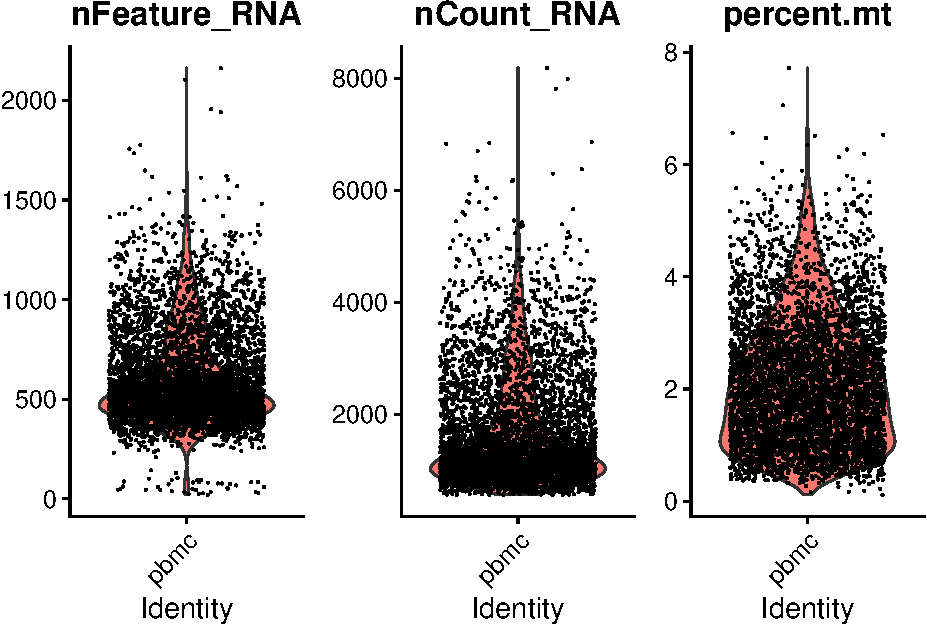
\includegraphics[keepaspectratio]{scRNAseqInR_ABACBS_2024_Doco_files/figure-latex/qc2-1.pdf}}

\begin{Shaded}
\begin{Highlighting}[]
\CommentTok{\# FeatureScatter is typically used to visualize feature{-}feature relationships, }
\CommentTok{\# but can be used for anything calculated by the object, }
\CommentTok{\# i.e. columns in object metadata, PC scores etc.}
\FunctionTok{FeatureScatter}\NormalTok{(seurat\_object, }\AttributeTok{feature1 =} \StringTok{"nCount\_RNA"}\NormalTok{, }\AttributeTok{feature2 =} \StringTok{"percent.mt"}\NormalTok{) }
\end{Highlighting}
\end{Shaded}

\pandocbounded{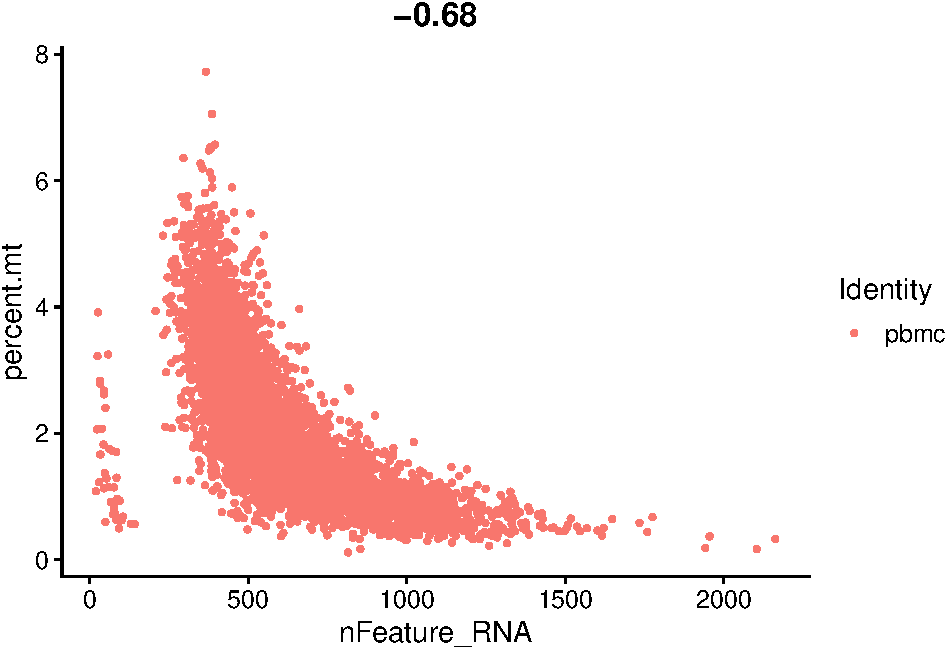
\includegraphics[keepaspectratio]{scRNAseqInR_ABACBS_2024_Doco_files/figure-latex/unnamed-chunk-12-1.pdf}}

\begin{Shaded}
\begin{Highlighting}[]
\FunctionTok{FeatureScatter}\NormalTok{(seurat\_object, }\AttributeTok{feature1 =} \StringTok{"nCount\_RNA"}\NormalTok{, }\AttributeTok{feature2 =} \StringTok{"nFeature\_RNA"}\NormalTok{) }
\end{Highlighting}
\end{Shaded}

\pandocbounded{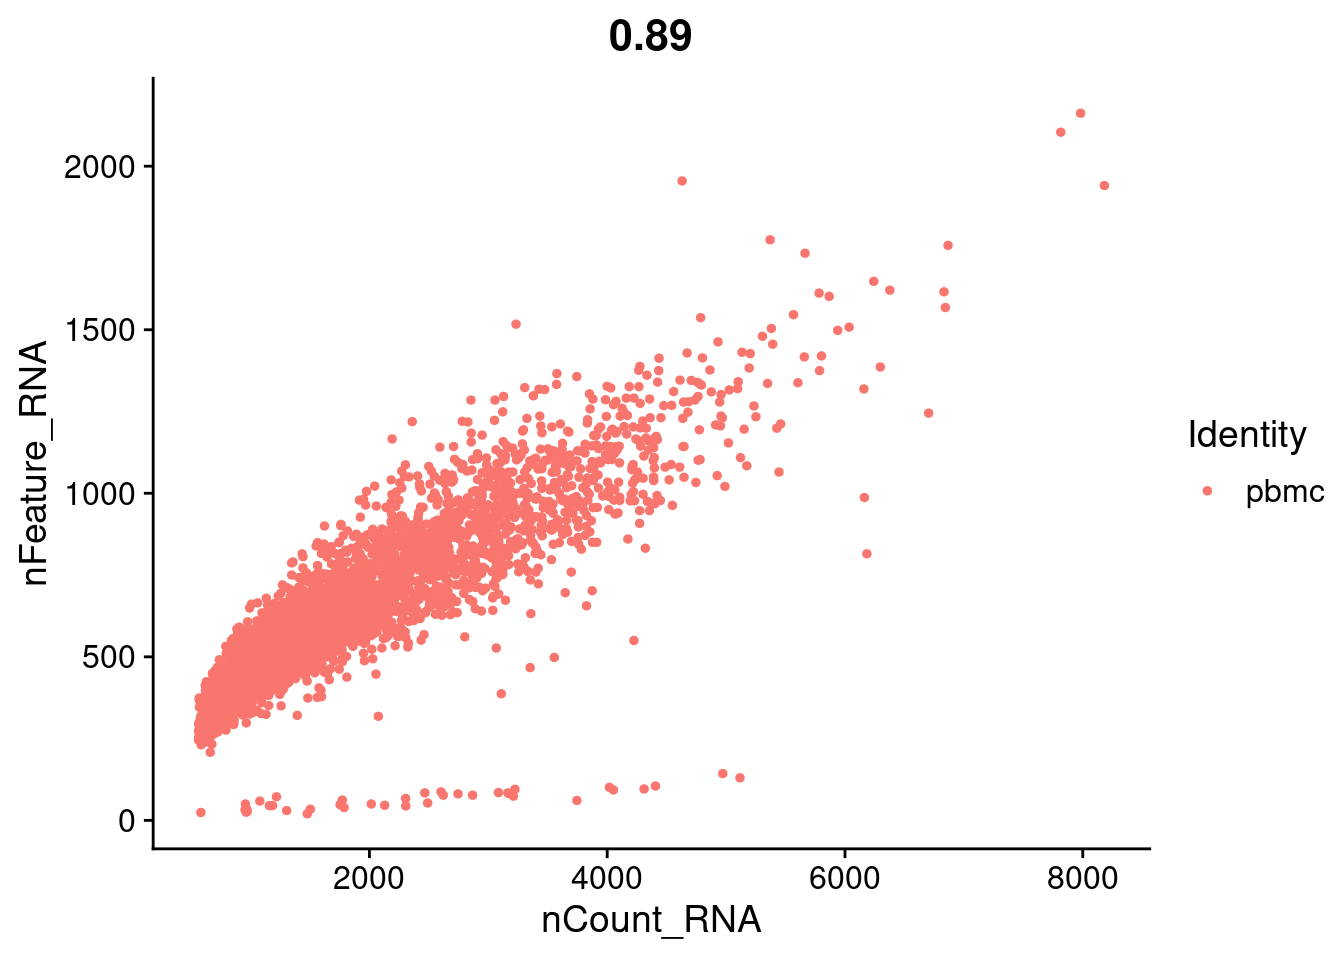
\includegraphics[keepaspectratio]{scRNAseqInR_ABACBS_2024_Doco_files/figure-latex/unnamed-chunk-12-2.pdf}}

\subsubsection*{Challenge: Red Blood Cells}\label{challenge-red-blood-cells}
\addcontentsline{toc}{subsubsection}{Challenge: Red Blood Cells}

Genes ``HBA1'', ``HBA2'', and ``HBB'' are components of hemoglobin in red blood cells.

\begin{itemize}
\tightlist
\item
  Use PercentageFeatureSet, passing these genes to the ``features'' argument, to find cells that might be red blood cells.
\item
  How do cells high in these genes differ from other cells, in terms of number of features or total count?
\item
  Should we remove these cells?
\end{itemize}

\subsubsection*{}\label{section-3}
\addcontentsline{toc}{subsubsection}{}

Let's look again at the number of features (genes) to the percent mitochondrial genes plot.

\begin{Shaded}
\begin{Highlighting}[]
\FunctionTok{VlnPlot}\NormalTok{(seurat\_object, }\AttributeTok{features =} \StringTok{"nFeature\_RNA"}\NormalTok{)}
\CommentTok{\#\textgreater{} Warning: Default search for "data" layer in "RNA" assay}
\CommentTok{\#\textgreater{} yielded no results; utilizing "counts" layer instead.}
\end{Highlighting}
\end{Shaded}

\pandocbounded{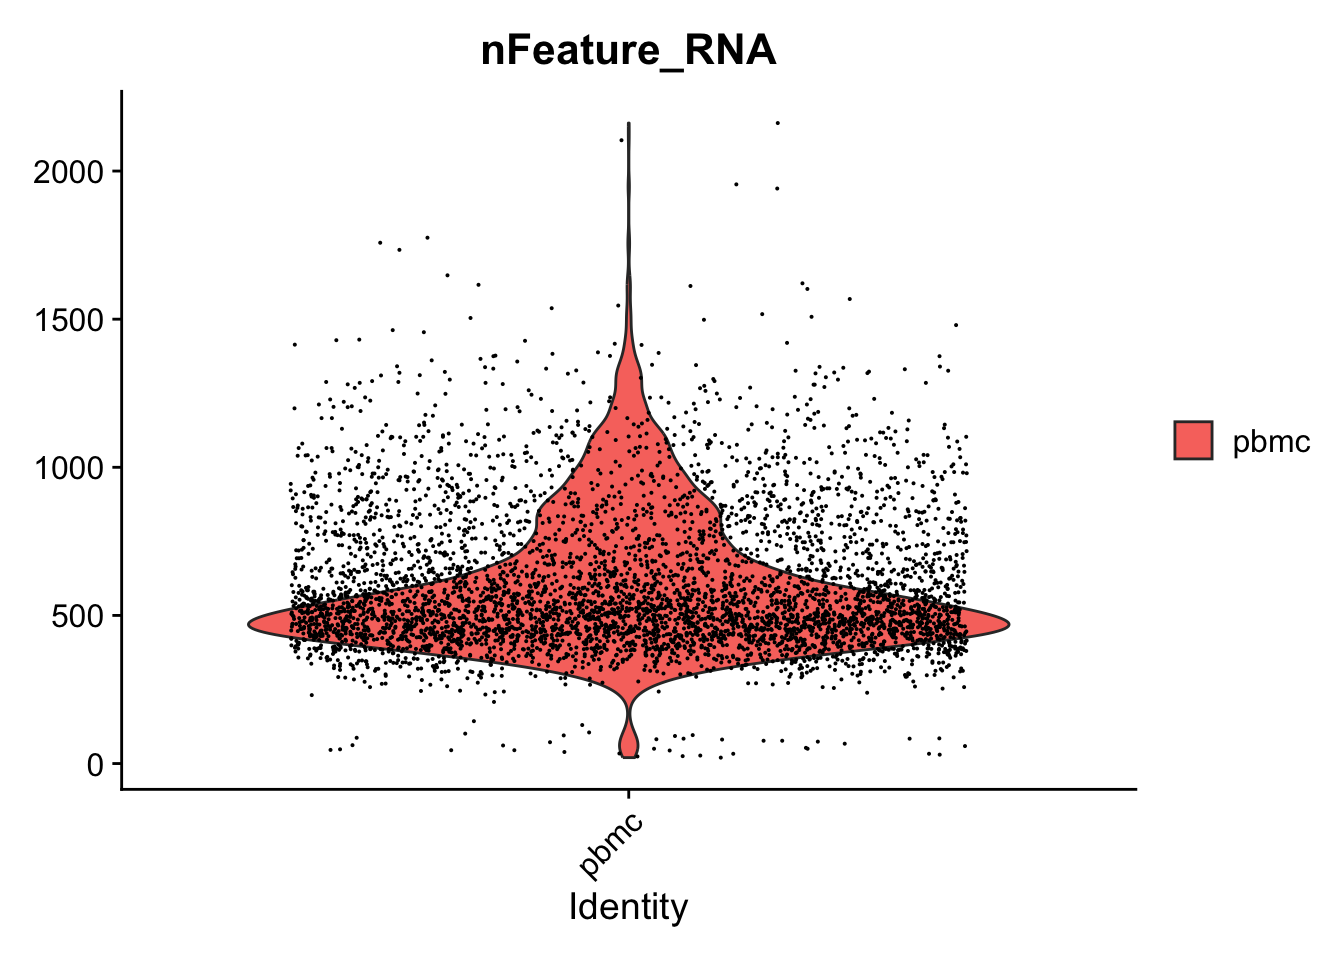
\includegraphics[keepaspectratio]{scRNAseqInR_ABACBS_2024_Doco_files/figure-latex/unnamed-chunk-13-1.pdf}}

\begin{Shaded}
\begin{Highlighting}[]

\CommentTok{\# Zoom in to the max and min }
\FunctionTok{VlnPlot}\NormalTok{(seurat\_object, }\AttributeTok{features =} \StringTok{"nFeature\_RNA"}\NormalTok{) }\SpecialCharTok{+} \FunctionTok{scale\_y\_continuous}\NormalTok{(}\AttributeTok{limits =} \FunctionTok{c}\NormalTok{(}\DecValTok{1000}\NormalTok{,}\DecValTok{3000}\NormalTok{))}
\CommentTok{\#\textgreater{} Warning: Default search for "data" layer in "RNA" assay}
\CommentTok{\#\textgreater{} yielded no results; utilizing "counts" layer instead.}
\CommentTok{\#\textgreater{} Scale for y is already present.}
\CommentTok{\#\textgreater{} Adding another scale for y, which will replace the existing}
\CommentTok{\#\textgreater{} scale.}
\CommentTok{\#\textgreater{} Warning: Removed 4624 rows containing non{-}finite outside the scale}
\CommentTok{\#\textgreater{} range (\textasciigrave{}stat\_ydensity()\textasciigrave{}).}
\CommentTok{\#\textgreater{} Warning: Removed 4624 rows containing missing values or values}
\CommentTok{\#\textgreater{} outside the scale range (\textasciigrave{}geom\_point()\textasciigrave{}).}
\end{Highlighting}
\end{Shaded}

\pandocbounded{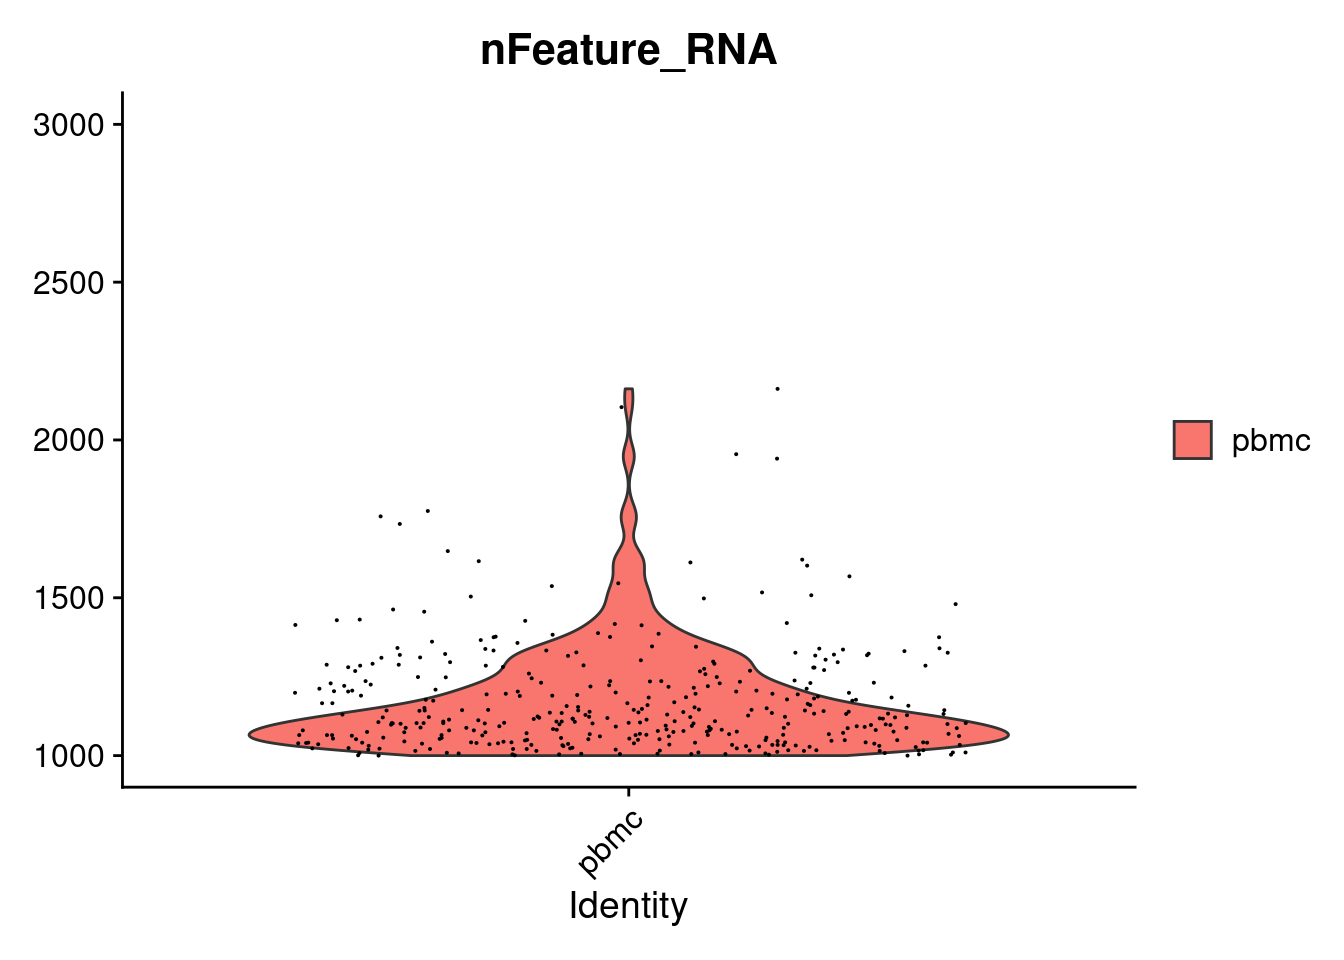
\includegraphics[keepaspectratio]{scRNAseqInR_ABACBS_2024_Doco_files/figure-latex/unnamed-chunk-13-2.pdf}}

\begin{Shaded}
\begin{Highlighting}[]
\FunctionTok{VlnPlot}\NormalTok{(seurat\_object, }\AttributeTok{features =} \StringTok{"nFeature\_RNA"}\NormalTok{, }\AttributeTok{y.max =}\DecValTok{1000}\NormalTok{)}
\CommentTok{\#\textgreater{} Warning: Default search for "data" layer in "RNA" assay}
\CommentTok{\#\textgreater{} yielded no results; utilizing "counts" layer instead.}
\CommentTok{\#\textgreater{} Warning: Removed 376 rows containing non{-}finite outside the scale}
\CommentTok{\#\textgreater{} range (\textasciigrave{}stat\_ydensity()\textasciigrave{}).}
\CommentTok{\#\textgreater{} Warning: Removed 376 rows containing missing values or values}
\CommentTok{\#\textgreater{} outside the scale range (\textasciigrave{}geom\_point()\textasciigrave{}).}
\end{Highlighting}
\end{Shaded}

\pandocbounded{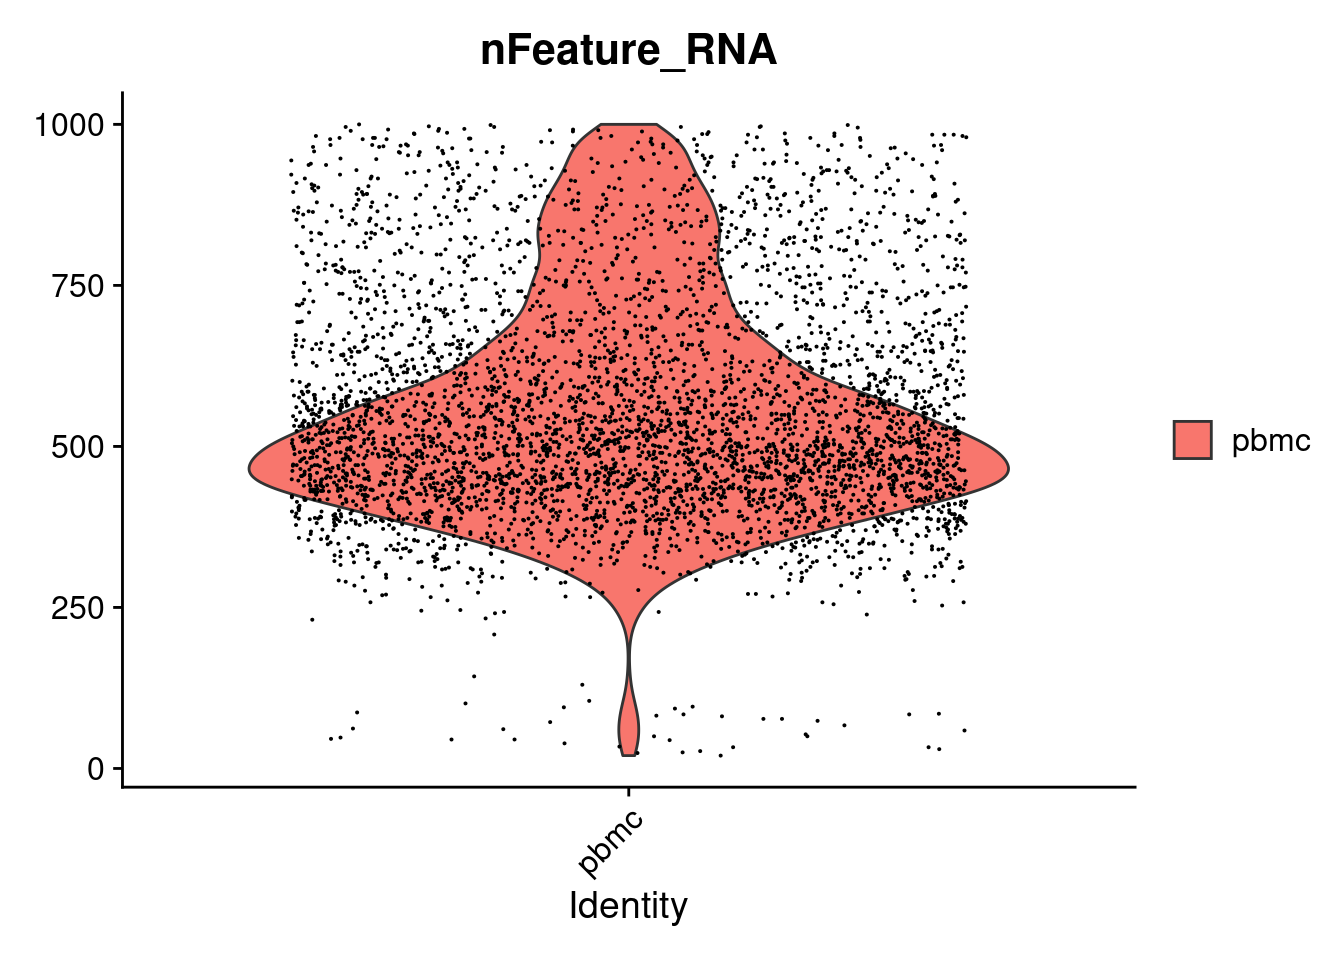
\includegraphics[keepaspectratio]{scRNAseqInR_ABACBS_2024_Doco_files/figure-latex/unnamed-chunk-13-3.pdf}}

\begin{Shaded}
\begin{Highlighting}[]

\FunctionTok{FeatureScatter}\NormalTok{(seurat\_object, }\AttributeTok{feature1 =} \StringTok{"nFeature\_RNA"}\NormalTok{, }\AttributeTok{feature2 =} \StringTok{"percent.mt"}\NormalTok{) }
\end{Highlighting}
\end{Shaded}

\pandocbounded{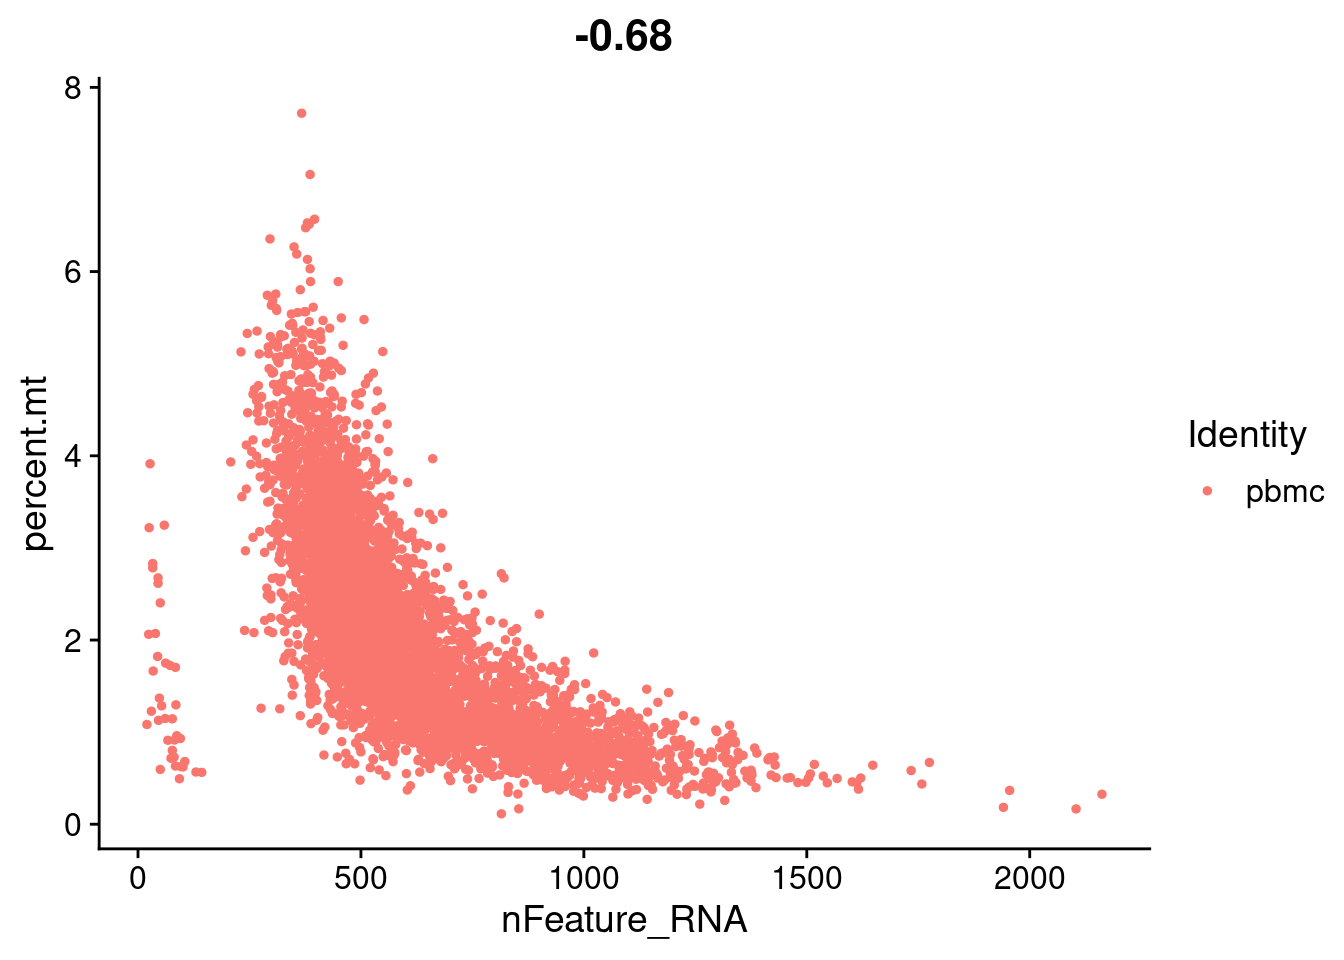
\includegraphics[keepaspectratio]{scRNAseqInR_ABACBS_2024_Doco_files/figure-latex/unnamed-chunk-13-4.pdf}}

You can check different thresholds of mito percentage.

\begin{Shaded}
\begin{Highlighting}[]
\CommentTok{\#Number of cells that would be left after filters}
\CommentTok{\# Proportion of cells with less than 5\% mito}

\FunctionTok{mean}\NormalTok{(seurat\_object}\SpecialCharTok{$}\NormalTok{percent.mt }\SpecialCharTok{\textless{}} \DecValTok{5}\NormalTok{) }
\CommentTok{\#\textgreater{} [1] 0.983}

\CommentTok{\# Proportion of cells with less than 2\% mito}

\FunctionTok{mean}\NormalTok{(seurat\_object}\SpecialCharTok{$}\NormalTok{percent.mt }\SpecialCharTok{\textless{}} \DecValTok{2}\NormalTok{)}
\CommentTok{\#\textgreater{} [1] 0.5158}
\end{Highlighting}
\end{Shaded}

Ok, let's go with these filters:

\begin{itemize}
\tightlist
\item
  We filter cells to have \textgreater200 unique features
\item
  We filter cells that have \textgreater5\% mitochondrial counts
\end{itemize}

Let's apply this and subset our data. This will remove the cells we think are of poor quality.

\begin{Shaded}
\begin{Highlighting}[]
\NormalTok{seurat\_object }\OtherTok{\textless{}{-}} \FunctionTok{subset}\NormalTok{(seurat\_object, }\AttributeTok{subset =}\NormalTok{ nFeature\_RNA }\SpecialCharTok{\textgreater{}} \DecValTok{200} \SpecialCharTok{\&}\NormalTok{ percent.mt }\SpecialCharTok{\textless{}} \DecValTok{5}\NormalTok{)}
\end{Highlighting}
\end{Shaded}

Let's replot the feature scatters and see what they look like.

\begin{Shaded}
\begin{Highlighting}[]
\FunctionTok{FeatureScatter}\NormalTok{(seurat\_object, }\AttributeTok{feature1 =} \StringTok{"nCount\_RNA"}\NormalTok{, }\AttributeTok{feature2 =} \StringTok{"percent.mt"}\NormalTok{) }
\end{Highlighting}
\end{Shaded}

\pandocbounded{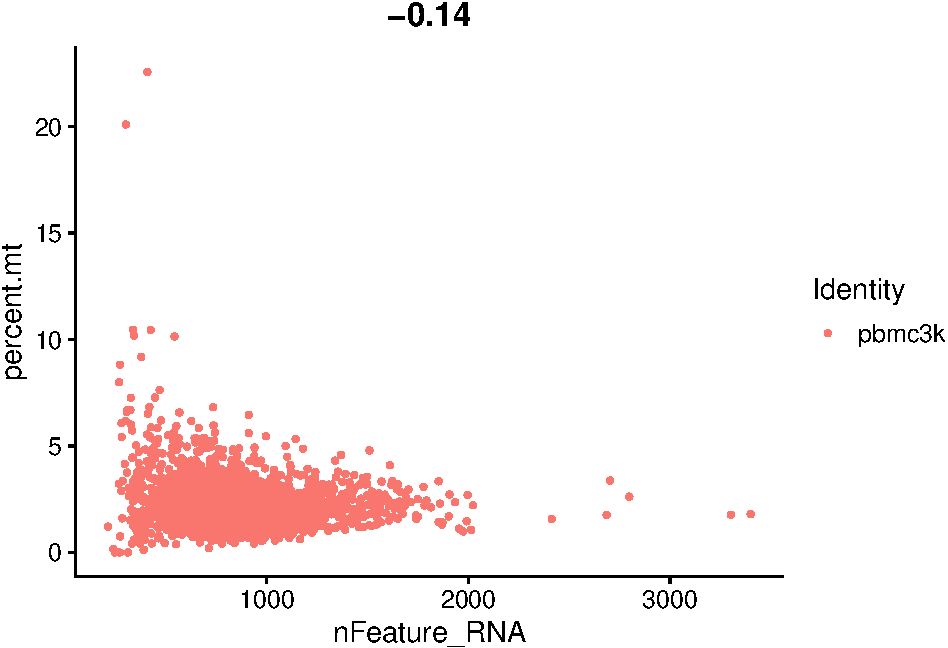
\includegraphics[keepaspectratio]{scRNAseqInR_ABACBS_2024_Doco_files/figure-latex/unnamed-chunk-16-1.pdf}}

\begin{Shaded}
\begin{Highlighting}[]
\FunctionTok{FeatureScatter}\NormalTok{(seurat\_object, }\AttributeTok{feature1 =} \StringTok{"nCount\_RNA"}\NormalTok{, }\AttributeTok{feature2 =} \StringTok{"nFeature\_RNA"}\NormalTok{) }
\end{Highlighting}
\end{Shaded}

\pandocbounded{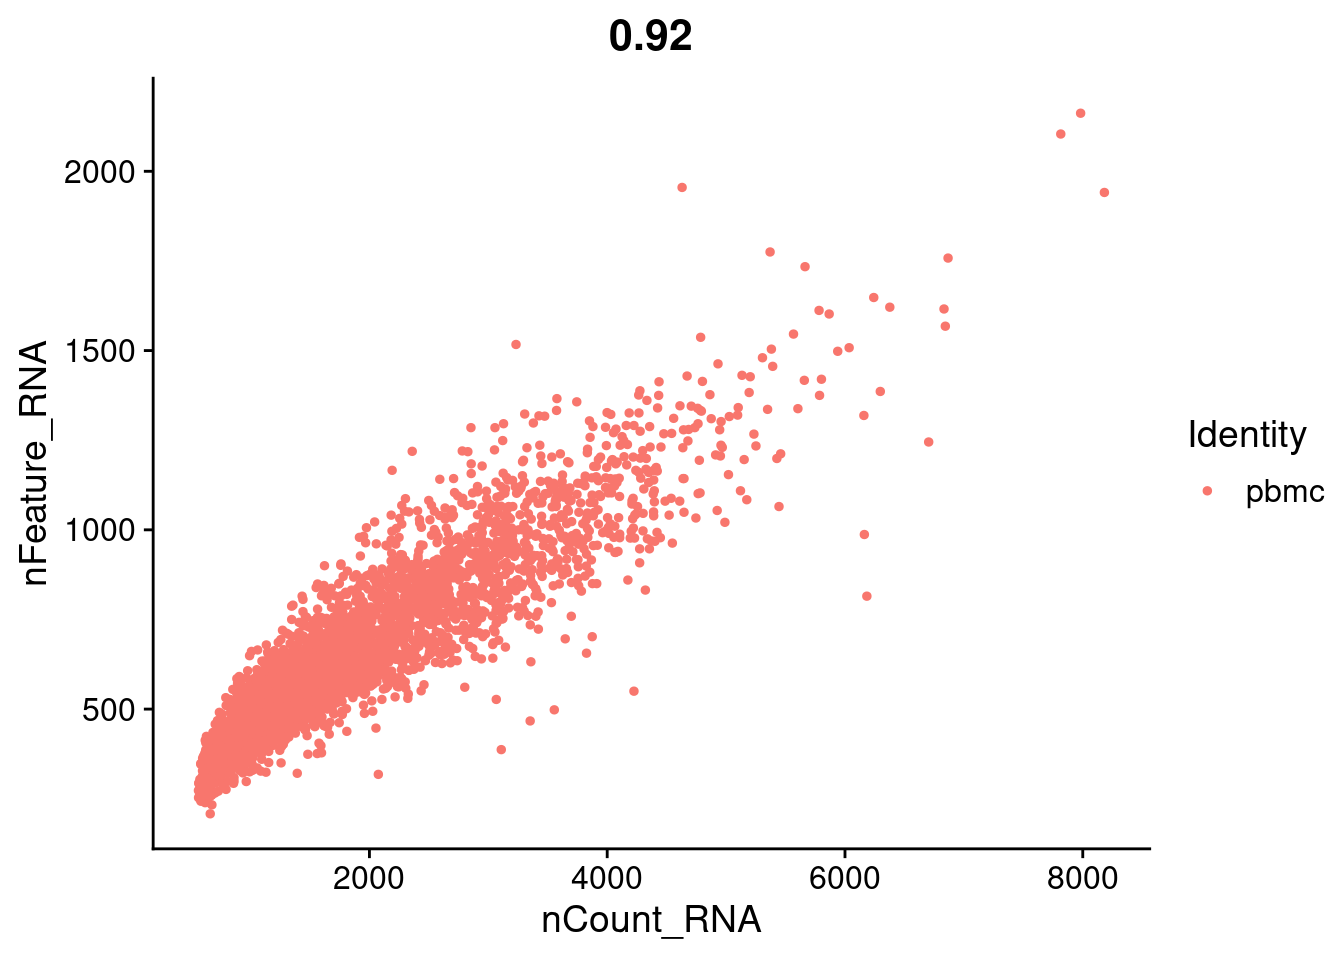
\includegraphics[keepaspectratio]{scRNAseqInR_ABACBS_2024_Doco_files/figure-latex/unnamed-chunk-16-2.pdf}}

We also wondered if cells with high counts might be doublets. Should we also filter cells with very high counts? With this data, we know for certain some of the doublets!

\begin{Shaded}
\begin{Highlighting}[]
\FunctionTok{FeatureScatter}\NormalTok{(seurat\_object, }\AttributeTok{feature1 =} \StringTok{"nCount\_RNA"}\NormalTok{, }\AttributeTok{feature2 =} \StringTok{"nFeature\_RNA"}\NormalTok{, }\AttributeTok{group.by=}\StringTok{"multiplets"}\NormalTok{) }
\end{Highlighting}
\end{Shaded}

\pandocbounded{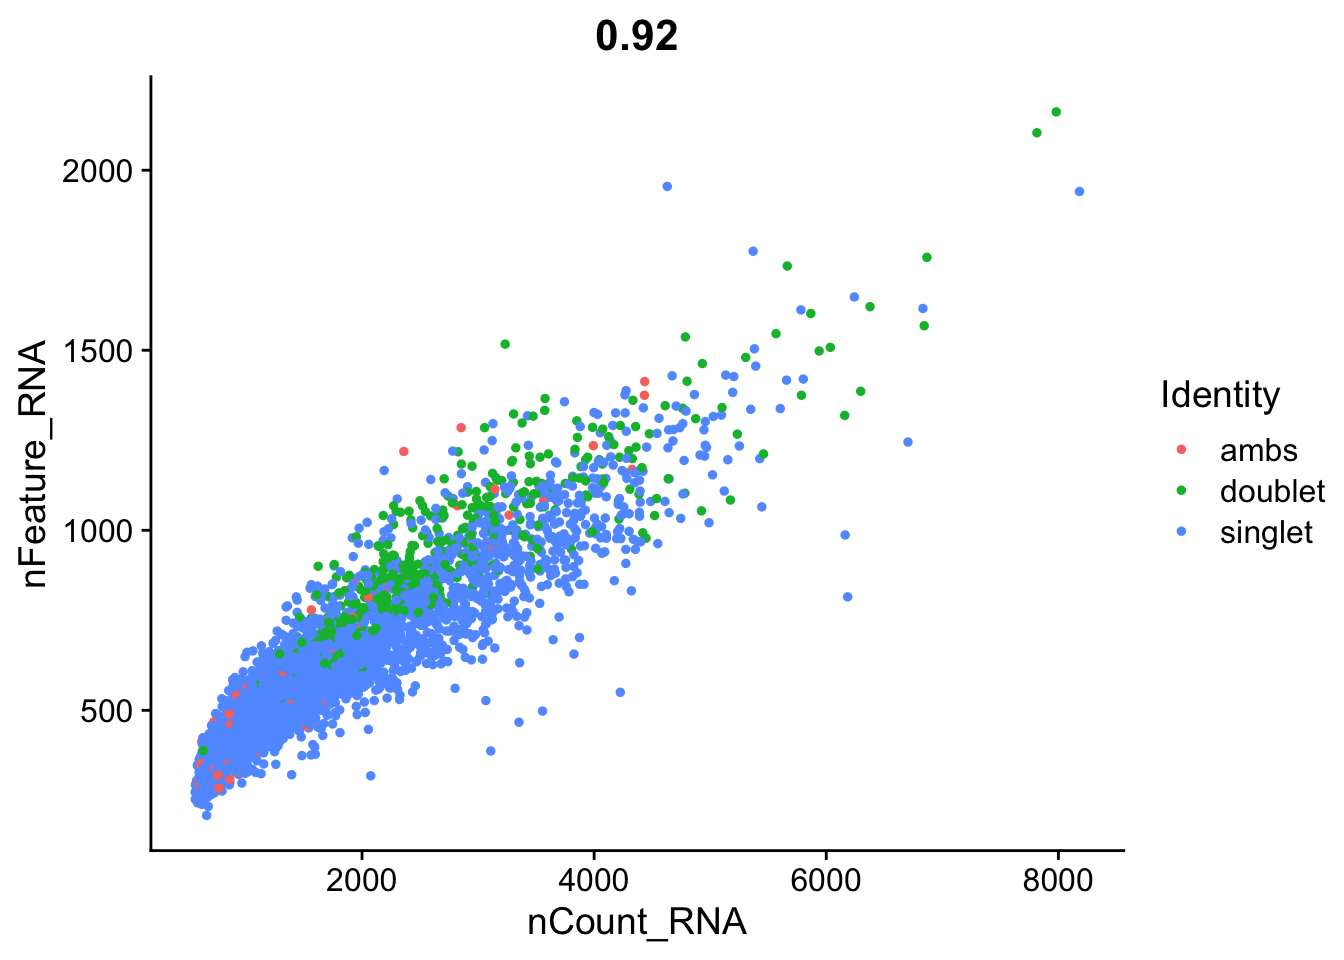
\includegraphics[keepaspectratio]{scRNAseqInR_ABACBS_2024_Doco_files/figure-latex/unnamed-chunk-17-1.pdf}}

\chapter{Normalisation}\label{norm}

\href{https://docs.google.com/presentation/d/1YAZPpgHyA6VhIWa4VeyyvfYYHnvaLt1b/edit\#slide=id.p1}{slides}

\subsubsection*{Why do we need to do this?}\label{why-do-we-need-to-do-this-1}
\addcontentsline{toc}{subsubsection}{Why do we need to do this?}

The sequencing depth can be different per cell. This can bias the counts of expression showing higher numbers for more sequenced cells leading to the wrong biological conclusions. To correct this the feature counts are normalized.

\subsubsection*{}\label{section-4}
\addcontentsline{toc}{subsubsection}{}

After removing unwanted cells from the dataset, the next step is to normalize the data. By default, we employ a global-scaling normalization method ``LogNormalize'' that normalizes the feature expression measurements for each cell by the total expression, multiplies this by a scale factor (10,000 by default), and log-transforms the result. Normalized values are stored in \texttt{seurat\_object\$RNA@data}.

\begin{Shaded}
\begin{Highlighting}[]
\NormalTok{seurat\_object }\OtherTok{\textless{}{-}} \FunctionTok{NormalizeData}\NormalTok{(seurat\_object, }\AttributeTok{normalization.method =} \StringTok{"LogNormalize"}\NormalTok{, }\AttributeTok{scale.factor =} \FloatTok{1e4}\NormalTok{)}
\CommentTok{\#\textgreater{} Normalizing layer: counts}
\end{Highlighting}
\end{Shaded}

For clarity, in this previous line of code (and in future commands), we provide the default values for certain parameters in the function call. However, this isn't required and the same behavior can be achieved with:

\begin{Shaded}
\begin{Highlighting}[]
\NormalTok{seurat\_object }\OtherTok{\textless{}{-}} \FunctionTok{NormalizeData}\NormalTok{(seurat\_object)}
\end{Highlighting}
\end{Shaded}

There are other options for normalization such as \href{https://genomebiology.biomedcentral.com/articles/10.1186/s13059-019-1874-1}{SCTtransform} which was popularized in 2019, however Log base normalization continued to be preferred as they perform better. \href{https://www.nature.com/articles/s41592-023-01814-1}{See here} for more details.

\chapter{PCAs and UMAPs}\label{reducedims}

\href{https://docs.google.com/presentation/d/17-AYqsosmKnJFgv_7DHYNbMQFIXrGAP4/edit\#slide=id.p1}{Slides}

\section{Identification of highly variable features (feature selection)}\label{identification-of-highly-variable-features-feature-selection}

\subsubsection*{Why do we need to do this?}\label{why-do-we-need-to-do-this-2}
\addcontentsline{toc}{subsubsection}{Why do we need to do this?}

Identifying the most variable features allows retaining the real biological variability of the data and reduce noise in the data.

\subsubsection*{}\label{section-5}
\addcontentsline{toc}{subsubsection}{}

We next calculate a subset of features that exhibit high cell-to-cell variation in the dataset (i.e, they are highly expressed in some cells, and lowly expressed in others). The Seurat authors and \href{https://www.nature.com/articles/nmeth.2645}{others} have found that focusing on these genes in downstream analysis helps to highlight biological signal in single-cell datasets.

The procedure in Seurat is described in detail \href{https://doi.org/10.1016/j.cell.2019.05.031}{here}, and improves on previous versions by directly modeling the mean-variance relationship inherent in single-cell data, and is implemented in the \texttt{FindVariableFeatures()} function. By default, Seurat returns 2,000 features per dataset. These will be used in downstream analysis, like PCA.

\begin{Shaded}
\begin{Highlighting}[]
\NormalTok{seurat\_object }\OtherTok{\textless{}{-}} \FunctionTok{FindVariableFeatures}\NormalTok{(seurat\_object, }\AttributeTok{selection.method =} \StringTok{\textquotesingle{}vst\textquotesingle{}}\NormalTok{, }\AttributeTok{nfeatures =} \DecValTok{2000}\NormalTok{)}
\CommentTok{\#\textgreater{} Finding variable features for layer counts}
\CommentTok{\# Identify the 10 most highly variable genes}
\NormalTok{top\_vf }\OtherTok{\textless{}{-}} \FunctionTok{head}\NormalTok{(}\FunctionTok{VariableFeatures}\NormalTok{(seurat\_object), }\DecValTok{10}\NormalTok{)}
\CommentTok{\# plot variable features with and without labels}
\NormalTok{plot1 }\OtherTok{\textless{}{-}} \FunctionTok{VariableFeaturePlot}\NormalTok{(seurat\_object)}
\NormalTok{plot2 }\OtherTok{\textless{}{-}} \FunctionTok{LabelPoints}\NormalTok{(plot1, }\AttributeTok{points =}\NormalTok{ top\_vf, }\AttributeTok{repel =} \ConstantTok{TRUE}\NormalTok{)}
\CommentTok{\#\textgreater{} When using repel, set xnudge and ynudge to 0 for optimal results}
\NormalTok{plot2}
\CommentTok{\#\textgreater{} Warning in scale\_x\_log10(): log{-}10 transformation}
\CommentTok{\#\textgreater{} introduced infinite values.}
\end{Highlighting}
\end{Shaded}

\pandocbounded{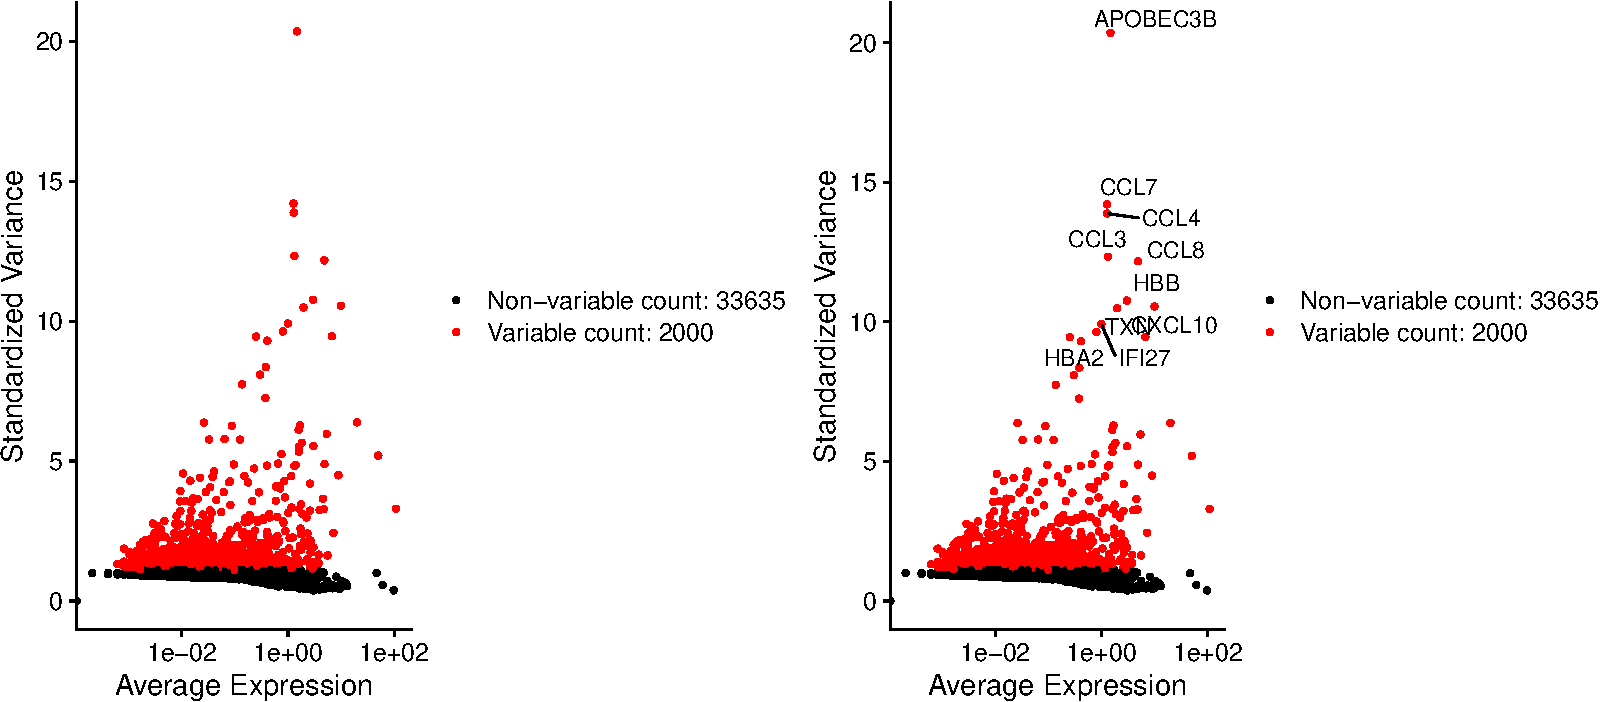
\includegraphics[keepaspectratio]{scRNAseqInR_ABACBS_2024_Doco_files/figure-latex/var_features-1.pdf}}

\section{Scaling the data}\label{scaling-the-data}

\subsubsection*{Why do we need to do this?}\label{why-do-we-need-to-do-this-3}
\addcontentsline{toc}{subsubsection}{Why do we need to do this?}

Highly expresed genes can overpower the signal of other less expresed genes with equal importance. Within the same cell the assumption is that the underlying RNA content is constant. Aditionally, If variables are provided in vars.to.regress, they are individually regressed against each feature, and the resulting residuals are then scaled and centered. This step allows controling for cell cycle and other factors that may bias your clustering.

\subsubsection*{}\label{section-6}
\addcontentsline{toc}{subsubsection}{}

Next, we apply a linear transformation (`scaling') that is a standard pre-processing step prior to dimensional reduction techniques like PCA. The \texttt{ScaleData()} function:

\begin{itemize}
\tightlist
\item
  Shifts the expression of each gene, so that the mean expression across cells is 0
\item
  Scales the expression of each gene, so that the variance across cells is 1

  \begin{itemize}
  \tightlist
  \item
    This step gives equal weight in downstream analyses, so that highly-expressed genes do not dominate
  \end{itemize}
\item
  The results of this are stored in \texttt{seurat\_object\$RNA@scale.data}
\end{itemize}

\begin{Shaded}
\begin{Highlighting}[]
\NormalTok{all.genes }\OtherTok{\textless{}{-}} \FunctionTok{rownames}\NormalTok{(seurat\_object)}
\NormalTok{seurat\_object }\OtherTok{\textless{}{-}} \FunctionTok{ScaleData}\NormalTok{(seurat\_object, }\AttributeTok{features =}\NormalTok{ all.genes)}
\CommentTok{\#\textgreater{} Centering and scaling data matrix}
\end{Highlighting}
\end{Shaded}

\textbf{This step takes too long! Can I make it faster?}

Scaling is an essential step in the Seurat workflow, but only on genes that will be used as input to PCA. Therefore, the default in \texttt{ScaleData()} is only to perform scaling on the previously identified variable features (2,000 by default). To do this, omit the \texttt{features} argument in the previous function call, i.e.

\begin{Shaded}
\begin{Highlighting}[]
\CommentTok{\# seurat\_object \textless{}{-} ScaleData(seurat\_object)}
\end{Highlighting}
\end{Shaded}

Your PCA and clustering results will be unaffected. However, Seurat heatmaps (produced as shown below with \texttt{DoHeatmap()}) require genes in the heatmap to be scaled, to make sure highly-expressed genes don't dominate the heatmap. To make sure we don't leave any genes out of the heatmap later, we are scaling all genes in this tutorial.

~

\textbf{How can I remove unwanted sources of variation, as in Seurat v2?}

In \texttt{Seurat\ v2} we also use the \texttt{ScaleData()} function to remove unwanted sources of variation from a single-cell dataset. For example, we could `regress out' heterogeneity associated with (for example) cell cycle stage, or mitochondrial contamination. These features are still supported in \texttt{ScaleData()} in \texttt{Seurat\ v3}, i.e.:

\begin{Shaded}
\begin{Highlighting}[]
\CommentTok{\# seurat\_object \textless{}{-} ScaleData(seurat\_object, vars.to.regress = \textquotesingle{}percent.mt\textquotesingle{})}
\end{Highlighting}
\end{Shaded}

However, particularly for advanced users who would like to use this functionality, the Seurat authors strongly recommend the use of their new normalization workflow, \texttt{SCTransform()}. The method is described in their \href{https://genomebiology.biomedcentral.com/articles/10.1186/s13059-019-1874-1}{paper}, with a separate vignette using Seurat v3 \href{sctransform_vignette.html}{here}. As with \texttt{ScaleData()}, the function \texttt{SCTransform()} also includes a \texttt{vars.to.regress} parameter.

~

\begin{center}\rule{0.5\linewidth}{0.5pt}\end{center}

\chapter{Dimensionality reduction}\label{dimensionality-reduction}

\subsubsection*{Why do we need to do this?}\label{why-do-we-need-to-do-this-4}
\addcontentsline{toc}{subsubsection}{Why do we need to do this?}

Imagine each gene represents a dimension - or an axis on a plot. We could plot the expression of two genes with a simple scatterplot. But a genome has thousands of genes - how do you collate all the information from each of those genes in a way that allows you to visualise it in a 2 dimensional image. This is where dimensionality reduction comes in, we calculate meta-features that contains combinations of the variation of different genes. From thousands of genes, we end up with 10s of meta-features

\subsubsection*{}\label{section-7}
\addcontentsline{toc}{subsubsection}{}

\section{Perform linear dimensional reduction}\label{perform-linear-dimensional-reduction}

Next we perform PCA on the scaled data. By default, only the previously determined variable features are used as input, but can be defined using \texttt{features} argument if you wish to choose a different subset.

\begin{Shaded}
\begin{Highlighting}[]
\NormalTok{seurat\_object }\OtherTok{\textless{}{-}} \FunctionTok{RunPCA}\NormalTok{(seurat\_object, }\AttributeTok{features =} \FunctionTok{VariableFeatures}\NormalTok{(}\AttributeTok{object =}\NormalTok{ seurat\_object))}
\CommentTok{\#\textgreater{} PC\_ 1 }
\CommentTok{\#\textgreater{} Positive:  CCR7, TRAT1, CREM, ALOX5AP, NKG7, TSC22D3, CST7, PASK, GPR171, CD8A }
\CommentTok{\#\textgreater{}     CD8B, ADTRP, SVIP, PRF1, MYC, NOP58, TTC39C, SESN3, CMTM8, C14orf1 }
\CommentTok{\#\textgreater{}     GRAP2, GZMA, TARBP1, KLRD1, CD320, GCHFR, AMICA1, TUBA4A, DDIT4, NOB1 }
\CommentTok{\#\textgreater{} Negative:  TYROBP, SOD2, TIMP1, TYMP, ANXA5, LGALS3, KYNU, FCN1, LYZ, APOBEC3A }
\CommentTok{\#\textgreater{}     CD68, NPC2, S100A11, CTSL, MAFB, HLA{-}DRA, SDCBP, S100A10, PLAUR, GSTO1 }
\CommentTok{\#\textgreater{}     IL4I1, IDO1, PILRA, LILRB4, S100A9, MS4A7, FGL2, CXCL11, HLA{-}DRB1, C3AR1 }
\CommentTok{\#\textgreater{} PC\_ 2 }
\CommentTok{\#\textgreater{} Positive:  CD14, S100A8, PID1, CD9, GPX1, THBS1, PLAUR, C19orf59, OSM, CTB{-}61M7.2 }
\CommentTok{\#\textgreater{}     MGST1, S100A9, GAPDH, C5AR1, SLC7A11, ATP6V0B, PPIF, CXCL2, TGFBI, PFN1 }
\CommentTok{\#\textgreater{}     LIMS1, OLR1, PLIN2, TIMP1, COTL1, CYP1B1, PDLIM7, SLC11A1, CYP27A1, CEBPB }
\CommentTok{\#\textgreater{} Negative:  IFIT3, MX1, TNFSF10, IFIT2, IFI6, RSAD2, OAS1, CXCL11, MT2A, IRF7 }
\CommentTok{\#\textgreater{}     IFITM3, OASL, GBP1, IDO1, PLSCR1, DDX58, CMPK2, APOBEC3A, FAM26F, BST2 }
\CommentTok{\#\textgreater{}     HES4, IFIH1, RABGAP1L, IL27, VAMP5, SERPING1, GMPR, SPATS2L, IRG1, IL4I1 }
\CommentTok{\#\textgreater{} PC\_ 3 }
\CommentTok{\#\textgreater{} Positive:  HLA{-}DQA1, CD83, HLA{-}DQB1, HLA{-}DRB1, HLA{-}DRA, HLA{-}DMA, HERPUD1, HSP90AB1, CCR7, ID3 }
\CommentTok{\#\textgreater{}     PKIB, TCF4, FABP5, BANK1, HSPD1, CLIC2, CD79B, FSCN1, HSPH1, CMTM6 }
\CommentTok{\#\textgreater{}     SQLE, TNFRSF13B, CD40, ALDH2, LY9, NME1, CKS2, HSP90AA1, HAPLN3, IGLL5 }
\CommentTok{\#\textgreater{} Negative:  ANXA1, NKG7, PRF1, GZMA, KLRD1, MT2A, S100A8, S100A9, OASL, CD300E }
\CommentTok{\#\textgreater{}     CST7, C3AR1, CD8A, TYROBP, CD14, S100A12, S100A6, FCGR3A, CTSL, FCN1 }
\CommentTok{\#\textgreater{}     MAFB, GCHFR, KLRC1, S100A11, IFI6, C5AR1, AQP9, FPR1, C19orf59, CD8B }
\CommentTok{\#\textgreater{} PC\_ 4 }
\CommentTok{\#\textgreater{} Positive:  CCR7, ADTRP, TRAT1, MYC, CMTM8, PASK, TARBP1, CTSL, SOCS3, S100A9 }
\CommentTok{\#\textgreater{}     S100A8, EMP3, SGTB, TSC22D3, FBLN7, SESN3, GBP1, NEXN, NPC2, MPRIP }
\CommentTok{\#\textgreater{}     HSP90AB1, IL27, S100A12, CCR1, PPA1, FCN1, SOD2, RSAD2, GPR171, HSPD1 }
\CommentTok{\#\textgreater{} Negative:  NKG7, CST7, PRF1, KLRD1, GZMA, ID2, KLRC1, TNFRSF18, RAMP1, IGFBP7 }
\CommentTok{\#\textgreater{}     ALOX5AP, CD8A, GCHFR, GNG2, GAPDH, FCGR3A, XCL2, ANXA1, PRR5L, OASL }
\CommentTok{\#\textgreater{}     RAB27A, HAVCR2, EIF4EBP1, PKIB, RHOC, GZMK, LINC00996, ADAM8, GSN, BST2 }
\CommentTok{\#\textgreater{} PC\_ 5 }
\CommentTok{\#\textgreater{} Positive:  FCGR3A, MS4A4A, MS4A7, CXCL16, PPM1N, SMPDL3A, AIF1, SERPINA1, ADA, CDKN1C }
\CommentTok{\#\textgreater{}     CH25H, C3AR1, PLAC8, IL3RA, PILRA, CFD, CLEC12A, VMP1, FGL2, VNN2 }
\CommentTok{\#\textgreater{}     FCGR3B, MTMR11, C1QA, MAPKAPK3, LILRB2, COTL1, FAM26F, FPR2, IFNGR2, IL15 }
\CommentTok{\#\textgreater{} Negative:  S100A9, MGST1, SLC7A11, S100A8, P2RY6, CCR5, LYZ, FPR3, RSAD2, FABP5 }
\CommentTok{\#\textgreater{}     SDS, EMP1, IFI6, CCR1, DHRS9, PRF1, CSTB, MX1, LILRB4, SPHK1 }
\CommentTok{\#\textgreater{}     TGFBI, ANXA1, IDO1, CXCL2, CCNA1, HSP90B1, NKG7, CMPK2, S100A12, LPXN}
\end{Highlighting}
\end{Shaded}

Seurat provides several useful ways of visualizing both cells and features that define the PCA, including \texttt{VizDimReduction()}, \texttt{DimPlot()}, and \texttt{DimHeatmap()}

\begin{Shaded}
\begin{Highlighting}[]
\CommentTok{\# Examine and visualize PCA results a few different ways}
\FunctionTok{print}\NormalTok{(seurat\_object}\SpecialCharTok{$}\NormalTok{pca, }\AttributeTok{dims =} \DecValTok{1}\SpecialCharTok{:}\DecValTok{5}\NormalTok{, }\AttributeTok{nfeatures =} \DecValTok{5}\NormalTok{)}
\CommentTok{\#\textgreater{} PC\_ 1 }
\CommentTok{\#\textgreater{} Positive:  CCR7, TRAT1, CREM, ALOX5AP, NKG7 }
\CommentTok{\#\textgreater{} Negative:  TYROBP, SOD2, TIMP1, TYMP, ANXA5 }
\CommentTok{\#\textgreater{} PC\_ 2 }
\CommentTok{\#\textgreater{} Positive:  CD14, S100A8, PID1, CD9, GPX1 }
\CommentTok{\#\textgreater{} Negative:  IFIT3, MX1, TNFSF10, IFIT2, IFI6 }
\CommentTok{\#\textgreater{} PC\_ 3 }
\CommentTok{\#\textgreater{} Positive:  HLA{-}DQA1, CD83, HLA{-}DQB1, HLA{-}DRB1, HLA{-}DRA }
\CommentTok{\#\textgreater{} Negative:  ANXA1, NKG7, PRF1, GZMA, KLRD1 }
\CommentTok{\#\textgreater{} PC\_ 4 }
\CommentTok{\#\textgreater{} Positive:  CCR7, ADTRP, TRAT1, MYC, CMTM8 }
\CommentTok{\#\textgreater{} Negative:  NKG7, CST7, PRF1, KLRD1, GZMA }
\CommentTok{\#\textgreater{} PC\_ 5 }
\CommentTok{\#\textgreater{} Positive:  FCGR3A, MS4A4A, MS4A7, CXCL16, PPM1N }
\CommentTok{\#\textgreater{} Negative:  S100A9, MGST1, SLC7A11, S100A8, P2RY6}
\FunctionTok{VizDimLoadings}\NormalTok{(seurat\_object, }\AttributeTok{dims =} \DecValTok{1}\SpecialCharTok{:}\DecValTok{2}\NormalTok{, }\AttributeTok{reduction =} \StringTok{\textquotesingle{}pca\textquotesingle{}}\NormalTok{)}
\end{Highlighting}
\end{Shaded}

\pandocbounded{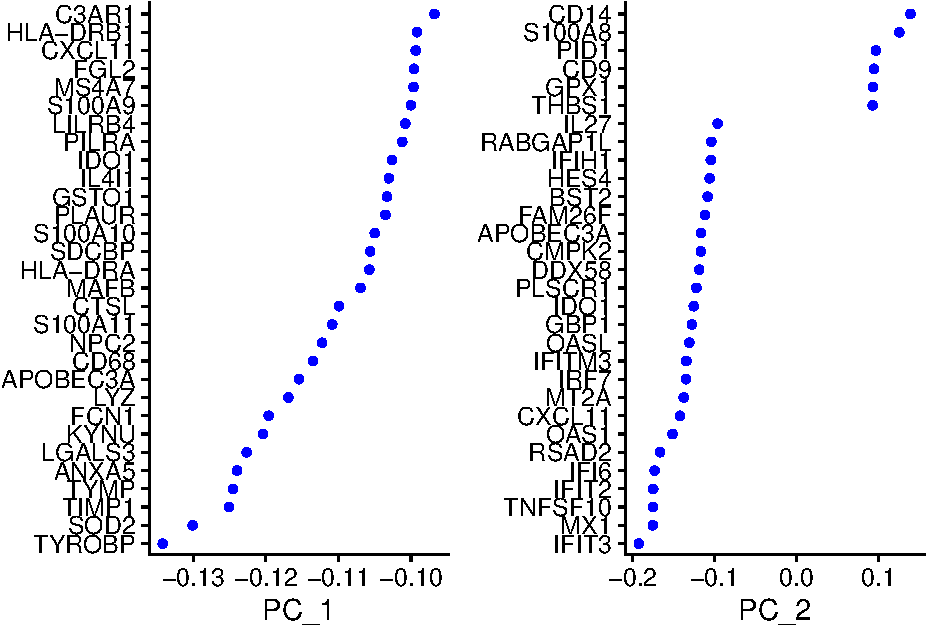
\includegraphics[keepaspectratio]{scRNAseqInR_ABACBS_2024_Doco_files/figure-latex/pca_viz-1.pdf}}

\begin{Shaded}
\begin{Highlighting}[]
\FunctionTok{DimPlot}\NormalTok{(seurat\_object, }\AttributeTok{reduction =} \StringTok{\textquotesingle{}pca\textquotesingle{}}\NormalTok{)}
\end{Highlighting}
\end{Shaded}

\pandocbounded{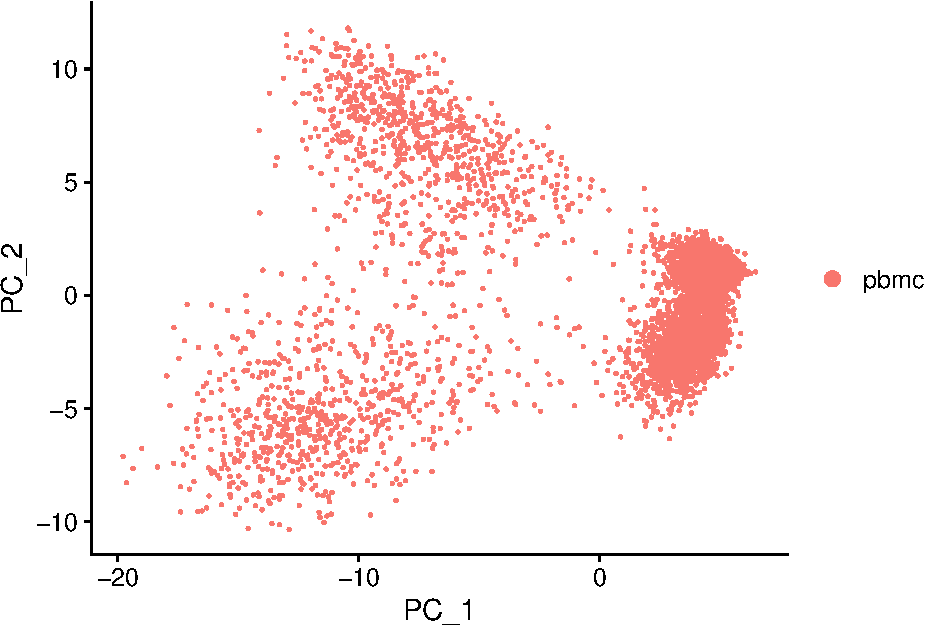
\includegraphics[keepaspectratio]{scRNAseqInR_ABACBS_2024_Doco_files/figure-latex/pca_viz-2.pdf}}

In particular \texttt{DimHeatmap()} allows for easy exploration of the primary sources of heterogeneity in a dataset, and can be useful when trying to decide which PCs to include for further downstream analyses. Both cells and features are ordered according to their PCA scores. Setting \texttt{cells} to a number plots the `extreme' cells on both ends of the spectrum, which dramatically speeds plotting for large datasets. Though clearly a supervised analysis, we find this to be a valuable tool for exploring correlated feature sets.

\begin{Shaded}
\begin{Highlighting}[]
\FunctionTok{DimHeatmap}\NormalTok{(seurat\_object, }\AttributeTok{dims =} \DecValTok{1}\NormalTok{, }\AttributeTok{cells =} \DecValTok{500}\NormalTok{, }\AttributeTok{balanced =} \ConstantTok{TRUE}\NormalTok{)}
\end{Highlighting}
\end{Shaded}

\pandocbounded{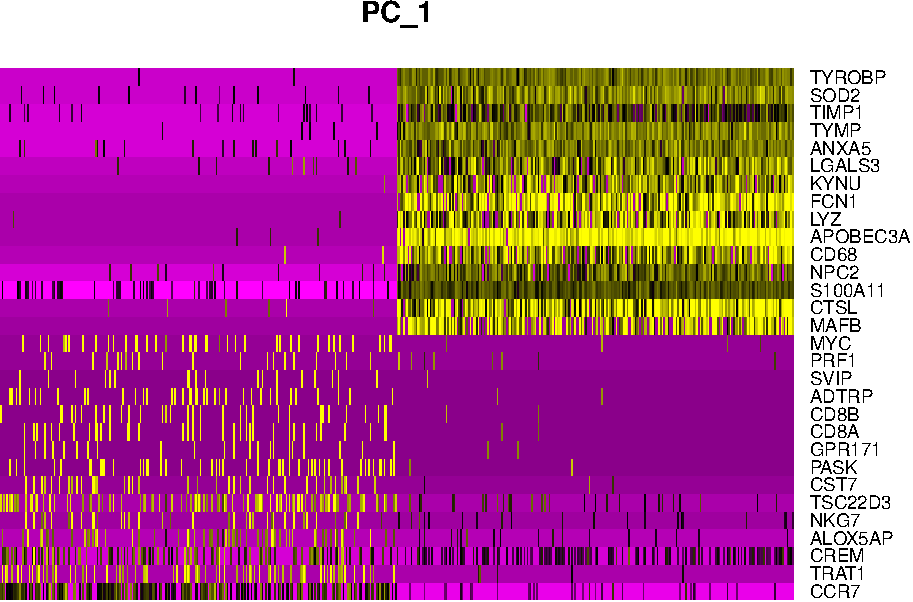
\includegraphics[keepaspectratio]{scRNAseqInR_ABACBS_2024_Doco_files/figure-latex/single-heatmap-1.pdf}}

\begin{Shaded}
\begin{Highlighting}[]
\FunctionTok{DimHeatmap}\NormalTok{(seurat\_object, }\AttributeTok{dims =} \DecValTok{1}\SpecialCharTok{:}\DecValTok{15}\NormalTok{, }\AttributeTok{cells =} \DecValTok{500}\NormalTok{, }\AttributeTok{balanced =} \ConstantTok{TRUE}\NormalTok{)}
\end{Highlighting}
\end{Shaded}

\pandocbounded{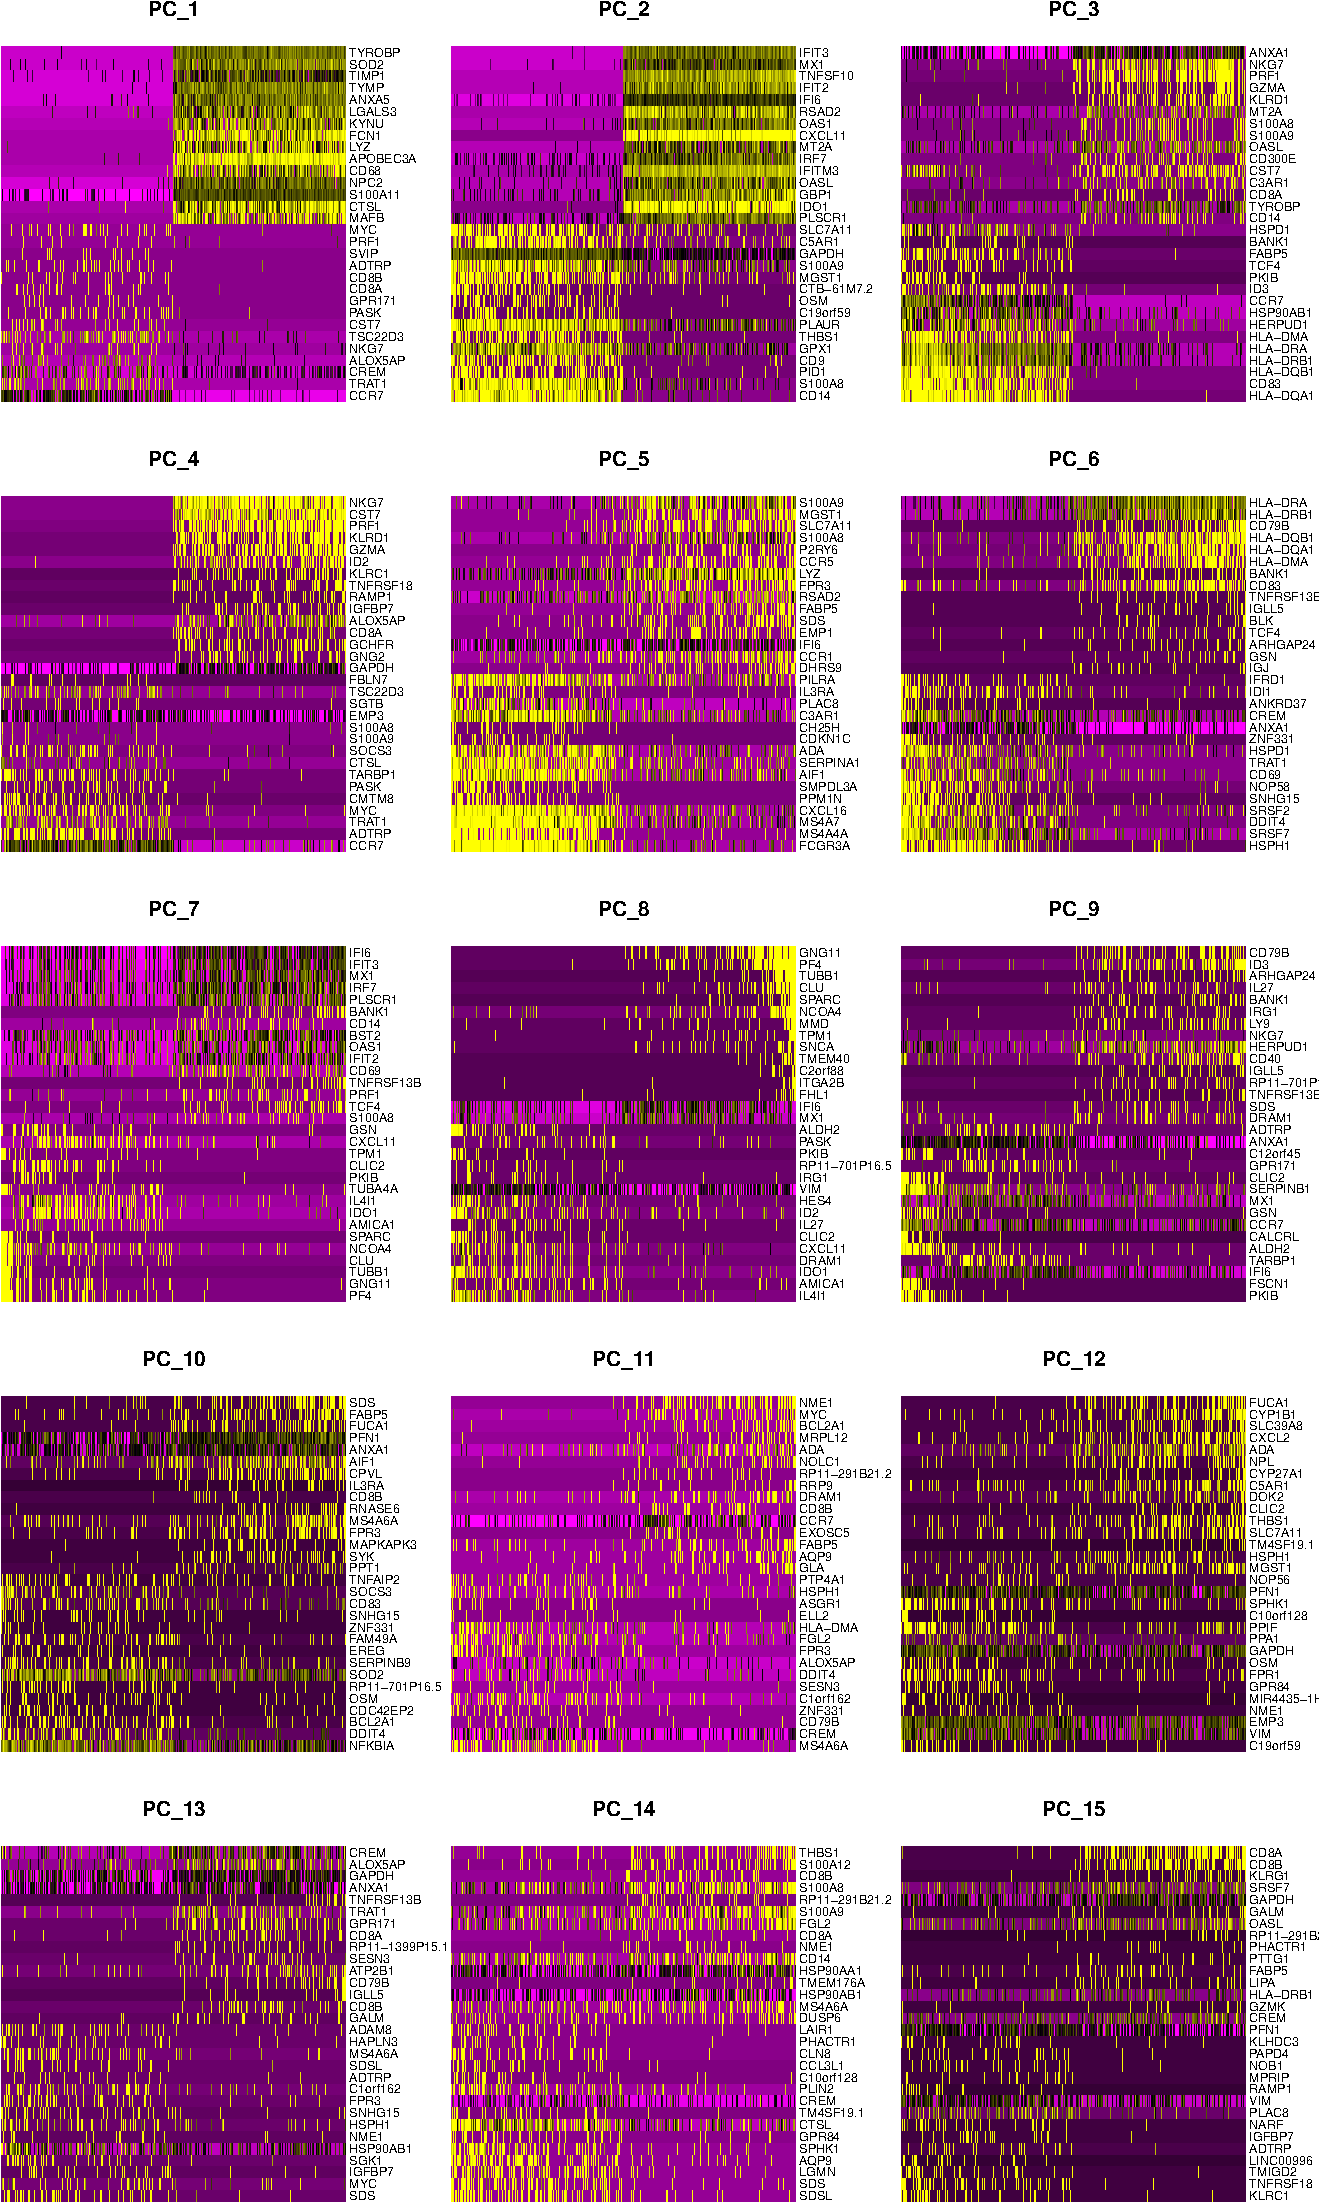
\includegraphics[keepaspectratio]{scRNAseqInR_ABACBS_2024_Doco_files/figure-latex/multi-heatmap-1.pdf}}

\section{Determine the `dimensionality' of the dataset}\label{determine-the-dimensionality-of-the-dataset}

To overcome the extensive technical noise in any single feature for scRNA-seq data, Seurat clusters cells based on their PCA scores, with each PC essentially representing a `metafeature' that combines information across a correlated feature set. The top principal components therefore represent a robust compression of the dataset. However, how many components should we choose to include? 10? 20? 100?

\begin{center}\rule{0.5\linewidth}{0.5pt}\end{center}

\emph{Note}: The Seurat developers suggest using a JackStraw resampling test to determine this. See \href{http://www.cell.com/abstract/S0092-8674(15)00549-8}{Macosko \emph{et al}}, and the original \href{https://satijalab.org/seurat/articles/seurat_object3k_tutorial.html\#determine-the-dimensionality-of-the-dataset-1}{seurat\_object3 vignette}. We're going to use an Elbow Plot instead here, because its much quicker.

\begin{center}\rule{0.5\linewidth}{0.5pt}\end{center}

An alternative heuristic method generates an `Elbow plot': a ranking of principle components based on the percentage of variance explained by each one (\texttt{ElbowPlot()} function). In this example, we can observe an `elbow' around PC9-10, suggesting that the majority of true signal is captured in the first 10 PCs.

\begin{Shaded}
\begin{Highlighting}[]
\FunctionTok{ElbowPlot}\NormalTok{(seurat\_object)}
\end{Highlighting}
\end{Shaded}

\pandocbounded{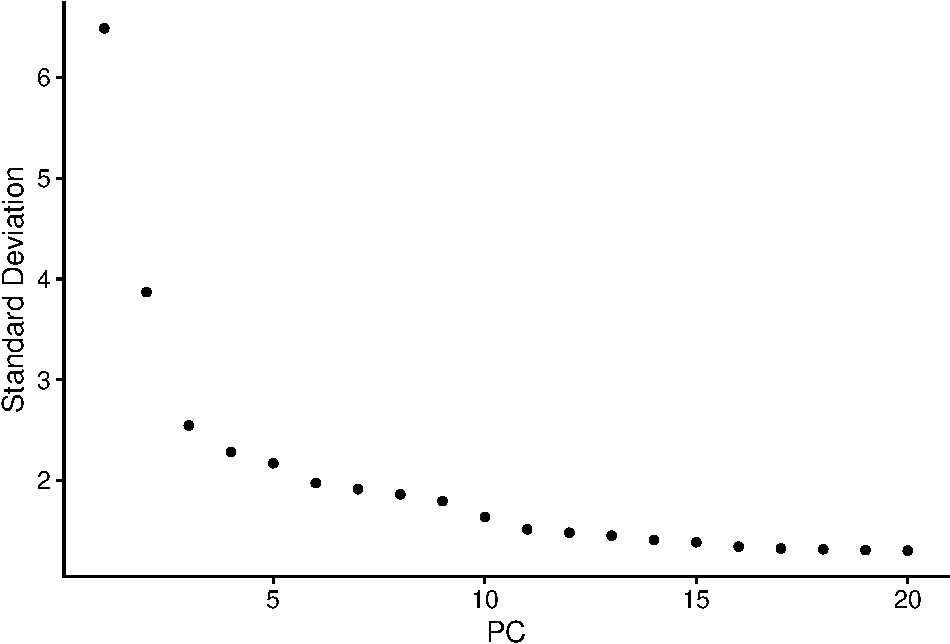
\includegraphics[keepaspectratio]{scRNAseqInR_ABACBS_2024_Doco_files/figure-latex/elbow_plot-1.pdf}}

Identifying the true dimensionality of a dataset -- can be challenging/uncertain for the user. We therefore suggest these three approaches to consider. The first is more supervised, exploring PCs to determine relevant sources of heterogeneity, and could be used in conjunction with GSEA for example. The second implements a statistical test based on a random null model, but is time-consuming for large datasets, and may not return a clear PC cutoff. The third is a heuristic that is commonly used, and can be calculated instantly. In this example, all three approaches yielded similar results, but we might have been justified in choosing anything between PC 7-12 as a cutoff.

We chose 10 here, but encourage users to consider the following:

\begin{itemize}
\tightlist
\item
  In the original version of this vignette with the PBMC3k dataset, genes strongly associated with PCs 12 and 13 defined rare immune subsets (i.e.~MZB1 is a marker for plasmacytoid DCs). However, these groups are so rare, they are difficult to distinguish from background noise for a dataset of this size without prior knowledge.
\item
  We encourage users to repeat downstream analyses with a different number of PCs (10, 15, or even 50!). As you will observe, the results often do not differ dramatically.
\item
  We advise users to err on the higher side when choosing this parameter. For example, performing downstream analyses with only 5 PCs does significantly and adversely affect results.
\end{itemize}

\begin{center}\rule{0.5\linewidth}{0.5pt}\end{center}

\section{Run non-linear dimensional reduction (UMAP/tSNE)}\label{run-non-linear-dimensional-reduction-umaptsne}

Seurat offers several non-linear dimensional reduction techniques, such as tSNE and UMAP, to visualize and explore these datasets. The goal of these algorithms is to learn the underlying manifold of the data in order to place similar cells together in low-dimensional space. Cells within the graph-based clusters determined above should co-localize on these dimension reduction plots. As input to the UMAP and tSNE, we suggest using the same PCs as input to the clustering analysis.

\begin{Shaded}
\begin{Highlighting}[]
\NormalTok{seurat\_object }\OtherTok{\textless{}{-}} \FunctionTok{RunUMAP}\NormalTok{(seurat\_object, }\AttributeTok{dims =} \DecValTok{1}\SpecialCharTok{:}\DecValTok{10}\NormalTok{)}
\CommentTok{\#\textgreater{} Warning: The default method for RunUMAP has changed from calling Python UMAP via reticulate to the R{-}native UWOT using the cosine metric}
\CommentTok{\#\textgreater{} To use Python UMAP via reticulate, set umap.method to \textquotesingle{}umap{-}learn\textquotesingle{} and metric to \textquotesingle{}correlation\textquotesingle{}}
\CommentTok{\#\textgreater{} This message will be shown once per session}
\CommentTok{\#\textgreater{} 23:33:13 UMAP embedding parameters a = 0.9922 b = 1.112}
\CommentTok{\#\textgreater{} 23:33:13 Read 4877 rows and found 10 numeric columns}
\CommentTok{\#\textgreater{} 23:33:13 Using Annoy for neighbor search, n\_neighbors = 30}
\CommentTok{\#\textgreater{} 23:33:13 Building Annoy index with metric = cosine, n\_trees = 50}
\CommentTok{\#\textgreater{} 0\%   10   20   30   40   50   60   70   80   90   100\%}
\CommentTok{\#\textgreater{} [{-}{-}{-}{-}|{-}{-}{-}{-}|{-}{-}{-}{-}|{-}{-}{-}{-}|{-}{-}{-}{-}|{-}{-}{-}{-}|{-}{-}{-}{-}|{-}{-}{-}{-}|{-}{-}{-}{-}|{-}{-}{-}{-}|}
\CommentTok{\#\textgreater{} **************************************************|}
\CommentTok{\#\textgreater{} 23:33:13 Writing NN index file to temp file /tmp/RtmporEusV/file1ab2d9648a275d}
\CommentTok{\#\textgreater{} 23:33:13 Searching Annoy index using 1 thread, search\_k = 3000}
\CommentTok{\#\textgreater{} 23:33:15 Annoy recall = 100\%}
\CommentTok{\#\textgreater{} 23:33:16 Commencing smooth kNN distance calibration using 1 thread with target n\_neighbors = 30}
\CommentTok{\#\textgreater{} 23:33:17 Initializing from normalized Laplacian + noise (using RSpectra)}
\CommentTok{\#\textgreater{} 23:33:17 Commencing optimization for 500 epochs, with 201470 positive edges}
\CommentTok{\#\textgreater{} 23:33:17 Using rng type: pcg}
\CommentTok{\#\textgreater{} 23:33:22 Optimization finished}
\end{Highlighting}
\end{Shaded}

\begin{Shaded}
\begin{Highlighting}[]
\FunctionTok{DimPlot}\NormalTok{(seurat\_object, }\AttributeTok{reduction =} \StringTok{\textquotesingle{}umap\textquotesingle{}}\NormalTok{)}
\end{Highlighting}
\end{Shaded}

\pandocbounded{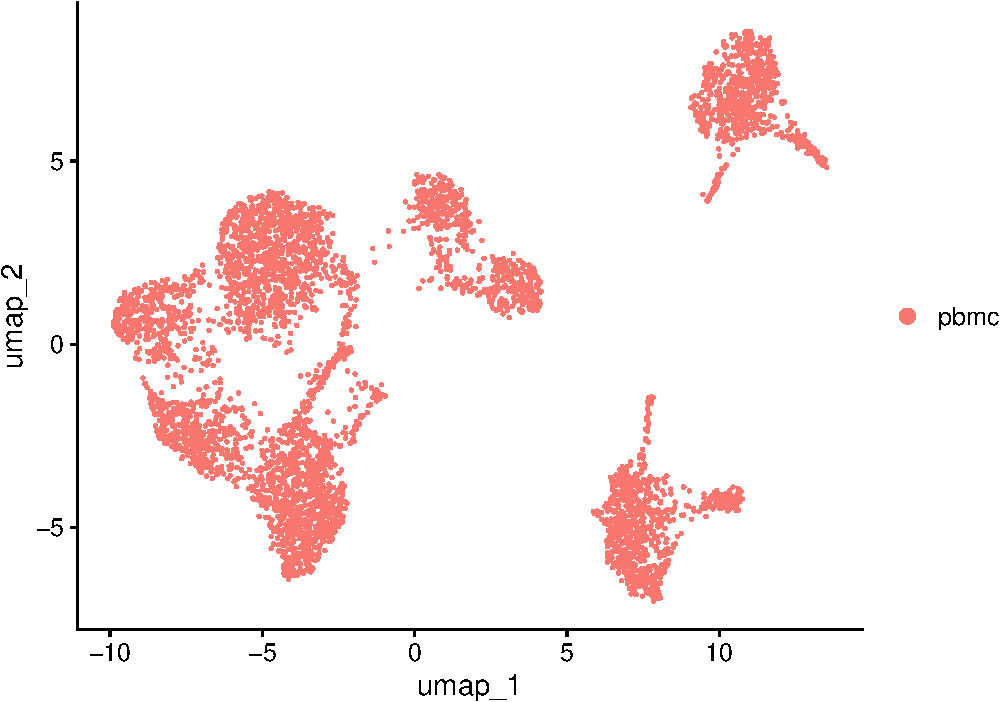
\includegraphics[keepaspectratio]{scRNAseqInR_ABACBS_2024_Doco_files/figure-latex/Umapplot-1.pdf}}

\subsubsection*{Challenge: PC genes}\label{challenge-pc-genes}
\addcontentsline{toc}{subsubsection}{Challenge: PC genes}

You can plot gene expression on the UMAP with the \texttt{FeaturePlot()} function.

Try out some genes that were highly weighted in the principal component analysis. How do they look?

\subsubsection*{}\label{section-8}
\addcontentsline{toc}{subsubsection}{}

\section{Save}\label{save}

You can save the object at this point so that it can easily be loaded back in with \texttt{readRDS()} without having to rerun the computationally intensive steps performed above, or easily shared with collaborators.

\begin{Shaded}
\begin{Highlighting}[]
\FunctionTok{saveRDS}\NormalTok{(seurat\_object, }\AttributeTok{file =} \StringTok{"seurat\_object\_tutorial\_saved.rds"}\NormalTok{) }
\end{Highlighting}
\end{Shaded}

Tip: For faster saving and loading, try the ``qs'' package.

\chapter{Data set integration with Harmony}\label{Harmony}

\href{https://docs.google.com/presentation/d/134p04OJPKy8yJQPwGtZ14HoLTbyN_flg/edit\#slide=id.p1}{Slides}

\subsection*{Why do we need to do this?}\label{why-do-we-need-to-do-this-5}
\addcontentsline{toc}{subsection}{Why do we need to do this?}

You can have data coming from different samples, batches or experiments and you will need to combine them.

\subsection*{}\label{section-9}
\addcontentsline{toc}{subsection}{}

\begin{itemize}
\tightlist
\item
  \texttt{ind} identifies a cell as coming from one of 8 individuals.
\item
  \texttt{stim} identifies a cell as control or stimulated with IFN-beta.
\item
  \texttt{cell} contains the cell types identified by the creators of this data set.
\item
  \texttt{multiplets} classifies cells as singlet or doublet.
\end{itemize}

\begin{Shaded}
\begin{Highlighting}[]
\FunctionTok{DimPlot}\NormalTok{(seurat\_object, }\AttributeTok{reduction=}\StringTok{"umap"}\NormalTok{, }\AttributeTok{group.by=}\StringTok{"ind"}\NormalTok{)}
\end{Highlighting}
\end{Shaded}

\pandocbounded{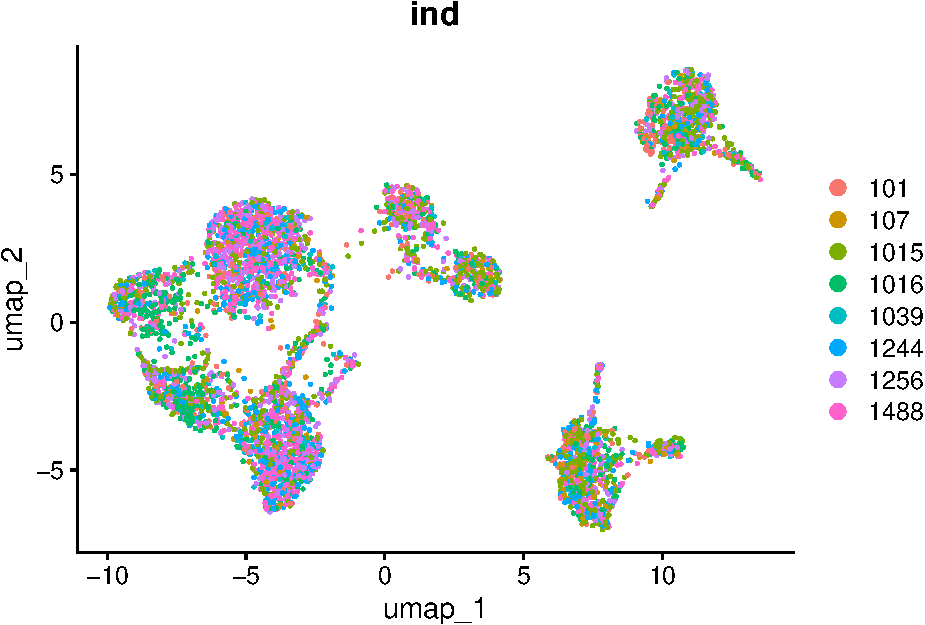
\includegraphics[keepaspectratio]{scRNAseqInR_ABACBS_2024_Doco_files/figure-latex/harmony1-1.pdf}}

\begin{Shaded}
\begin{Highlighting}[]
\FunctionTok{DimPlot}\NormalTok{(seurat\_object, }\AttributeTok{reduction=}\StringTok{"umap"}\NormalTok{, }\AttributeTok{group.by=}\StringTok{"stim"}\NormalTok{)}
\end{Highlighting}
\end{Shaded}

\pandocbounded{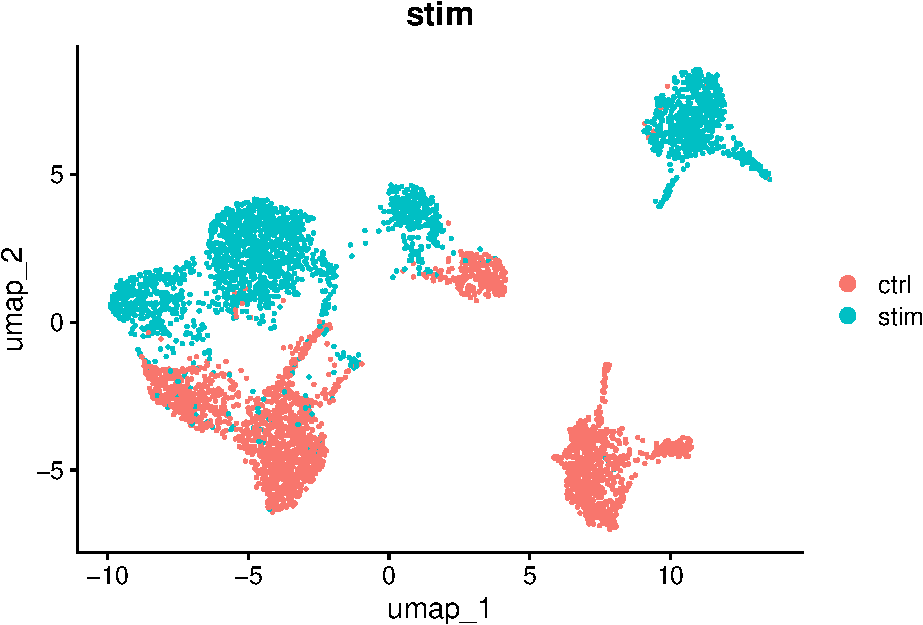
\includegraphics[keepaspectratio]{scRNAseqInR_ABACBS_2024_Doco_files/figure-latex/harmony1-2.pdf}}

\begin{Shaded}
\begin{Highlighting}[]

\NormalTok{seurat\_object}\OtherTok{\textless{}{-}} \FunctionTok{FindNeighbors}\NormalTok{(seurat\_object, }\AttributeTok{reduction=}\StringTok{"pca"}\NormalTok{, }\AttributeTok{dims=}\DecValTok{1}\SpecialCharTok{:}\DecValTok{10}\NormalTok{)}
\CommentTok{\#\textgreater{} Computing nearest neighbor graph}
\CommentTok{\#\textgreater{} Computing SNN}
\NormalTok{seurat\_object }\OtherTok{\textless{}{-}} \FunctionTok{FindClusters}\NormalTok{(seurat\_object, }\AttributeTok{resolution=}\FloatTok{0.5}\NormalTok{)}
\CommentTok{\#\textgreater{} Modularity Optimizer version 1.3.0 by Ludo Waltman and Nees Jan van Eck}
\CommentTok{\#\textgreater{} }
\CommentTok{\#\textgreater{} Number of nodes: 4877}
\CommentTok{\#\textgreater{} Number of edges: 171734}
\CommentTok{\#\textgreater{} }
\CommentTok{\#\textgreater{} Running Louvain algorithm...}
\CommentTok{\#\textgreater{} Maximum modularity in 10 random starts: 0.9108}
\CommentTok{\#\textgreater{} Number of communities: 13}
\CommentTok{\#\textgreater{} Elapsed time: 0 seconds}
\NormalTok{seurat\_object}\SpecialCharTok{$}\NormalTok{pca\_clusters }\OtherTok{\textless{}{-}}\NormalTok{ seurat\_object}\SpecialCharTok{$}\NormalTok{seurat\_clusters}

\FunctionTok{DimPlot}\NormalTok{(seurat\_object, }\AttributeTok{reduction=}\StringTok{"umap"}\NormalTok{, }\AttributeTok{group.by=}\StringTok{"pca\_clusters"}\NormalTok{)}
\end{Highlighting}
\end{Shaded}

\pandocbounded{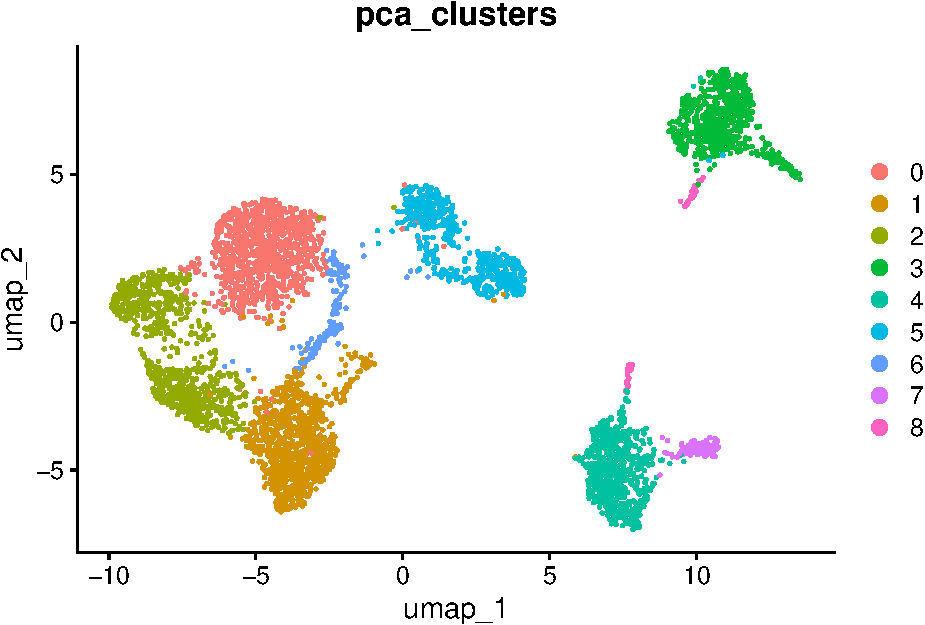
\includegraphics[keepaspectratio]{scRNAseqInR_ABACBS_2024_Doco_files/figure-latex/harmony1-3.pdf}}

There is a big difference between unstimulated and stimulated cells. This has split cells of the same type into pairs of clusters. If the difference was simply uniform, we could regress it out (e.g.~using \texttt{ScaleData(...,\ vars.to.regress="stim")}). However, as can be seen in the PCA plot, the difference is not uniform and we need to do something cleverer.

We will use \href{https://github.com/immunogenomics/harmony}{Harmony}, which can remove non-uniform effects. We will try to remove both the small differences between individuals and the large difference between the unstimulated and stimulated cells.

Harmony operates only on the PCA scores. The original gene expression levels remain unaltered.

\begin{Shaded}
\begin{Highlighting}[]
\FunctionTok{library}\NormalTok{(harmony)}
\CommentTok{\#\textgreater{} Loading required package: Rcpp}

\NormalTok{seurat\_object }\OtherTok{\textless{}{-}} \FunctionTok{RunHarmony}\NormalTok{(seurat\_object, }\FunctionTok{c}\NormalTok{(}\StringTok{"stim"}\NormalTok{, }\StringTok{"ind"}\NormalTok{), }\AttributeTok{reduction=}\StringTok{"pca"}\NormalTok{,}\AttributeTok{reduction.save=}\StringTok{"harmony"}\NormalTok{)}
\CommentTok{\#\textgreater{} Transposing data matrix}
\CommentTok{\#\textgreater{} Initializing state using k{-}means centroids initialization}
\CommentTok{\#\textgreater{} Harmony 1/10}
\CommentTok{\#\textgreater{} Harmony 2/10}
\CommentTok{\#\textgreater{} Harmony 3/10}
\CommentTok{\#\textgreater{} Harmony 4/10}
\CommentTok{\#\textgreater{} Harmony converged after 4 iterations}
\CommentTok{\#\textgreater{} Warning: The \textasciigrave{}slot\textasciigrave{} argument of \textasciigrave{}GetAssayData()\textasciigrave{} is deprecated as of}
\CommentTok{\#\textgreater{} SeuratObject 5.0.0.}
\CommentTok{\#\textgreater{} i Please use the \textasciigrave{}layer\textasciigrave{} argument instead.}
\CommentTok{\#\textgreater{} i The deprecated feature was likely used in the Seurat}
\CommentTok{\#\textgreater{}   package.}
\CommentTok{\#\textgreater{}   Please report the issue at}
\CommentTok{\#\textgreater{}   \textless{}https://github.com/satijalab/seurat/issues\textgreater{}.}
\CommentTok{\#\textgreater{} This warning is displayed once every 8 hours.}
\CommentTok{\#\textgreater{} Call \textasciigrave{}lifecycle::last\_lifecycle\_warnings()\textasciigrave{} to see where}
\CommentTok{\#\textgreater{} this warning was generated.}
\end{Highlighting}
\end{Shaded}

This has added a new set of reduced dimensions to the Seurat object, \texttt{seurat\_object\$harmony} which is a modified version of the existing \texttt{seurat\_object\$pca} reduced dimensions. The PCA plot shows a large difference between `ctrl' and `stim', but this has been removed in the harmony reduction.

\begin{Shaded}
\begin{Highlighting}[]
\FunctionTok{DimPlot}\NormalTok{(seurat\_object, }\AttributeTok{reduction=}\StringTok{"pca"}\NormalTok{, }\AttributeTok{group.by=}\StringTok{"stim"}\NormalTok{)}
\end{Highlighting}
\end{Shaded}

\pandocbounded{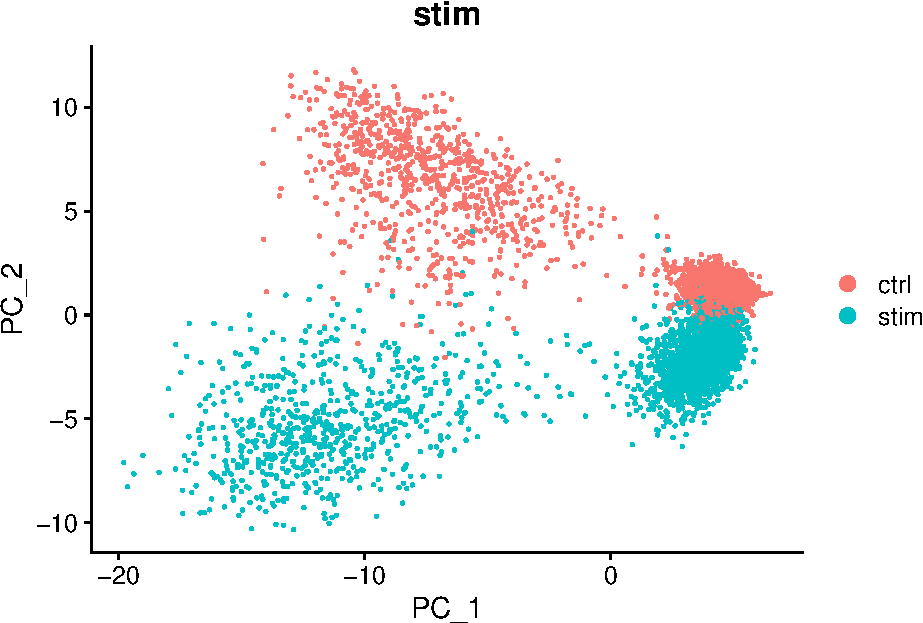
\includegraphics[keepaspectratio]{scRNAseqInR_ABACBS_2024_Doco_files/figure-latex/harmony3-1.pdf}}

\begin{Shaded}
\begin{Highlighting}[]
\FunctionTok{DimPlot}\NormalTok{(seurat\_object, }\AttributeTok{reduction=}\StringTok{"harmony"}\NormalTok{, }\AttributeTok{group.by=}\StringTok{"stim"}\NormalTok{)}
\end{Highlighting}
\end{Shaded}

\pandocbounded{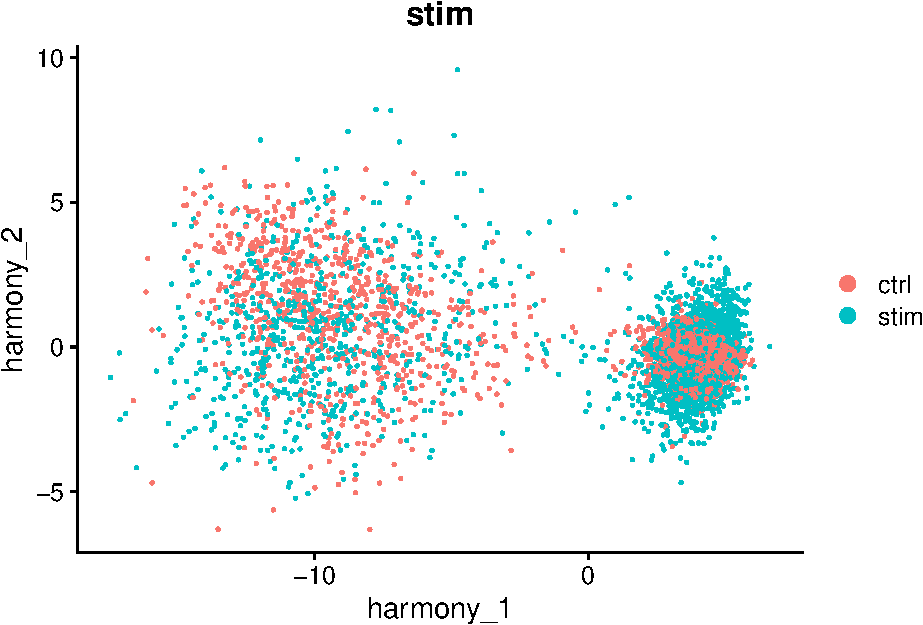
\includegraphics[keepaspectratio]{scRNAseqInR_ABACBS_2024_Doco_files/figure-latex/harmony3-2.pdf}}

We can use \texttt{harmony} the same way we used the \texttt{pca} reduction to compute a UMAP layout or to find clusters.

\begin{Shaded}
\begin{Highlighting}[]
\NormalTok{seurat\_object }\OtherTok{\textless{}{-}} \FunctionTok{RunUMAP}\NormalTok{(seurat\_object, }\AttributeTok{reduction=}\StringTok{"harmony"}\NormalTok{, }\AttributeTok{dims=}\DecValTok{1}\SpecialCharTok{:}\DecValTok{10}\NormalTok{, }\AttributeTok{reduction.name=}\StringTok{"umap\_harmony"}\NormalTok{)}
\CommentTok{\#\textgreater{} 23:33:49 UMAP embedding parameters a = 0.9922 b = 1.112}
\CommentTok{\#\textgreater{} 23:33:49 Read 4877 rows and found 10 numeric columns}
\CommentTok{\#\textgreater{} 23:33:49 Using Annoy for neighbor search, n\_neighbors = 30}
\CommentTok{\#\textgreater{} 23:33:49 Building Annoy index with metric = cosine, n\_trees = 50}
\CommentTok{\#\textgreater{} 0\%   10   20   30   40   50   60   70   80   90   100\%}
\CommentTok{\#\textgreater{} [{-}{-}{-}{-}|{-}{-}{-}{-}|{-}{-}{-}{-}|{-}{-}{-}{-}|{-}{-}{-}{-}|{-}{-}{-}{-}|{-}{-}{-}{-}|{-}{-}{-}{-}|{-}{-}{-}{-}|{-}{-}{-}{-}|}
\CommentTok{\#\textgreater{} **************************************************|}
\CommentTok{\#\textgreater{} 23:33:49 Writing NN index file to temp file /tmp/RtmporEusV/file1ab2d9146582e1}
\CommentTok{\#\textgreater{} 23:33:49 Searching Annoy index using 1 thread, search\_k = 3000}
\CommentTok{\#\textgreater{} 23:33:51 Annoy recall = 100\%}
\CommentTok{\#\textgreater{} 23:33:52 Commencing smooth kNN distance calibration using 1 thread with target n\_neighbors = 30}
\CommentTok{\#\textgreater{} 23:33:53 Initializing from normalized Laplacian + noise (using RSpectra)}
\CommentTok{\#\textgreater{} 23:33:53 Commencing optimization for 500 epochs, with 203710 positive edges}
\CommentTok{\#\textgreater{} 23:33:53 Using rng type: pcg}
\CommentTok{\#\textgreater{} 23:33:58 Optimization finished}

\FunctionTok{DimPlot}\NormalTok{(seurat\_object, }\AttributeTok{reduction=}\StringTok{"umap\_harmony"}\NormalTok{, }\AttributeTok{group.by=}\StringTok{"stim"}\NormalTok{)}
\end{Highlighting}
\end{Shaded}

\pandocbounded{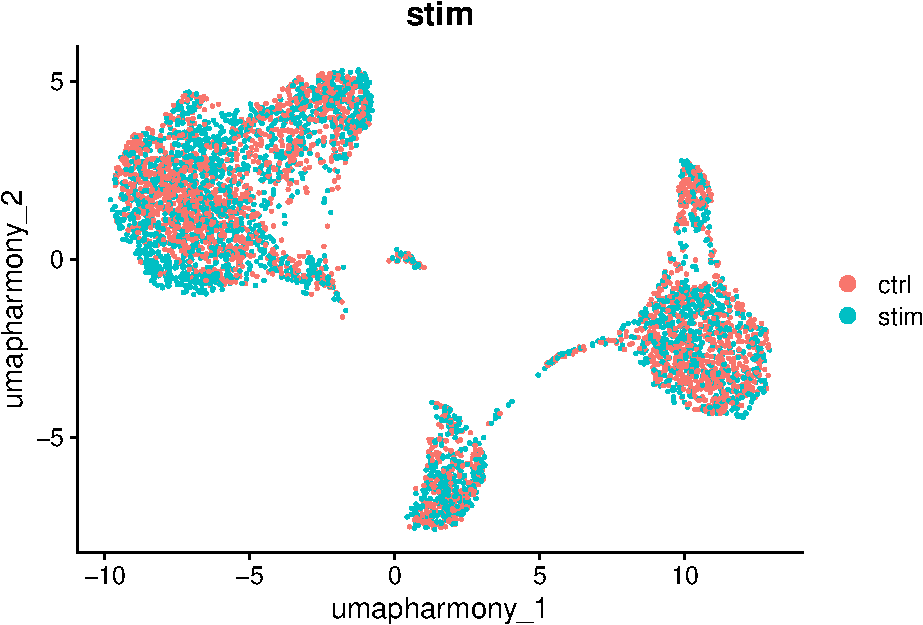
\includegraphics[keepaspectratio]{scRNAseqInR_ABACBS_2024_Doco_files/figure-latex/harmony4-1.pdf}}

\begin{Shaded}
\begin{Highlighting}[]

\NormalTok{seurat\_object }\OtherTok{\textless{}{-}} \FunctionTok{FindNeighbors}\NormalTok{(seurat\_object, }\AttributeTok{reduction=}\StringTok{"harmony"}\NormalTok{, }\AttributeTok{dims=}\DecValTok{1}\SpecialCharTok{:}\DecValTok{10}\NormalTok{)}
\CommentTok{\#\textgreater{} Computing nearest neighbor graph}
\CommentTok{\#\textgreater{} Computing SNN}
\NormalTok{seurat\_object }\OtherTok{\textless{}{-}} \FunctionTok{FindClusters}\NormalTok{(seurat\_object, }\AttributeTok{resolution=}\FloatTok{0.5}\NormalTok{)}
\CommentTok{\#\textgreater{} Modularity Optimizer version 1.3.0 by Ludo Waltman and Nees Jan van Eck}
\CommentTok{\#\textgreater{} }
\CommentTok{\#\textgreater{} Number of nodes: 4877}
\CommentTok{\#\textgreater{} Number of edges: 169427}
\CommentTok{\#\textgreater{} }
\CommentTok{\#\textgreater{} Running Louvain algorithm...}
\CommentTok{\#\textgreater{} Maximum modularity in 10 random starts: 0.8660}
\CommentTok{\#\textgreater{} Number of communities: 8}
\CommentTok{\#\textgreater{} Elapsed time: 0 seconds}
\NormalTok{seurat\_object}\SpecialCharTok{$}\NormalTok{harmony\_clusters }\OtherTok{\textless{}{-}}\NormalTok{ seurat\_object}\SpecialCharTok{$}\NormalTok{seurat\_clusters}

\FunctionTok{DimPlot}\NormalTok{(seurat\_object, }\AttributeTok{reduction=}\StringTok{"umap\_harmony"}\NormalTok{, }\AttributeTok{group.by=}\StringTok{"harmony\_clusters"}\NormalTok{)}
\end{Highlighting}
\end{Shaded}

\pandocbounded{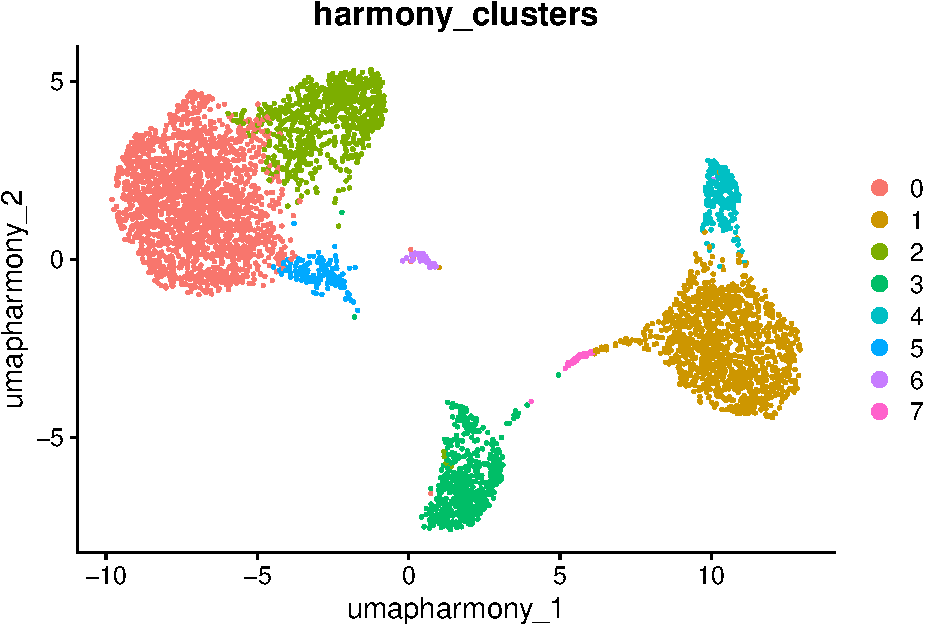
\includegraphics[keepaspectratio]{scRNAseqInR_ABACBS_2024_Doco_files/figure-latex/harmony4-2.pdf}}

\begin{Shaded}
\begin{Highlighting}[]
\FunctionTok{DimPlot}\NormalTok{(seurat\_object, }\AttributeTok{reduction=}\StringTok{"umap"}\NormalTok{, }\AttributeTok{group.by=}\StringTok{"harmony\_clusters"}\NormalTok{)}
\end{Highlighting}
\end{Shaded}

\pandocbounded{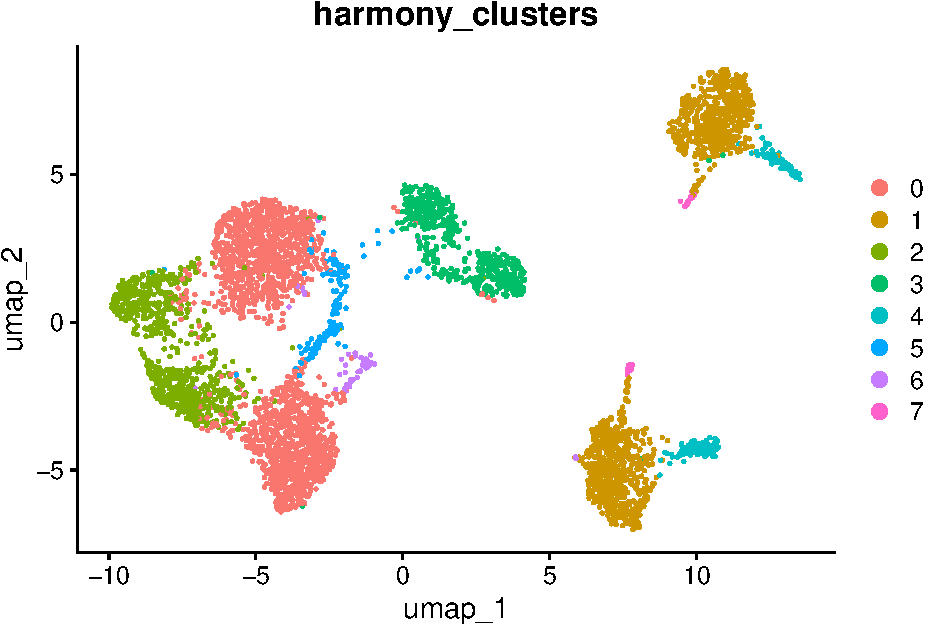
\includegraphics[keepaspectratio]{scRNAseqInR_ABACBS_2024_Doco_files/figure-latex/harmony4-3.pdf}}

Having found a good set of clusters, we would usually perform differential expression analysis on the original data and include batches/runs/individuals as predictors in the linear model. In this example we could now compare un-stimulated and stimulated cells within each cluster. A particularly nice statistical approach that is possible here would be to convert the counts to pseudo-bulk data for the eight individuals, and then apply a bulk RNA-Seq differential expression analysis method. However there is still the problem that unstimulated and stimulated cells were processed in separate batches.

\chapter{Clustering}\label{clustering}

\href{https://docs.google.com/presentation/d/1erfD1gJAZwpyh2l8wkWBGzUiVStQCyL_/edit\#slide=id.p33}{Slides}

\subsubsection*{Why do we need to do this?}\label{why-do-we-need-to-do-this-6}
\addcontentsline{toc}{subsubsection}{Why do we need to do this?}

Clustering the cells will allow you to visualise the variability of your data, can help to segregate cells into cell types.

\subsubsection*{}\label{section-10}
\addcontentsline{toc}{subsubsection}{}

\section{Cluster cells}\label{cluster-cells}

Seurat v3 applies a graph-based clustering approach, building upon initial strategies in (\href{http://www.cell.com/abstract/S0092-8674(15)00549-8}{Macosko \emph{et al}}). Importantly, the \emph{distance metric} which drives the clustering analysis (based on previously identified PCs) remains the same. However, our approach to partitioning the cellular distance matrix into clusters has dramatically improved. Our approach was heavily inspired by recent manuscripts which applied graph-based clustering approaches to scRNA-seq data \href{http://bioinformatics.oxfordjournals.org/content/early/2015/02/10/bioinformatics.btv088.abstract}{{[}SNN-Cliq, Xu and Su, Bioinformatics, 2015{]}} and CyTOF data \href{http://www.ncbi.nlm.nih.gov/pubmed/26095251}{{[}PhenoGraph, Levine \emph{et al}., Cell, 2015{]}}. Briefly, these methods embed cells in a graph structure - for example a K-nearest neighbor (KNN) graph, with edges drawn between cells with similar feature expression patterns, and then attempt to partition this graph into highly interconnected `quasi-cliques' or `communities'.

As in PhenoGraph, we first construct a KNN graph based on the euclidean distance in PCA space, and refine the edge weights between any two cells based on the shared overlap in their local neighborhoods (Jaccard similarity). This step is performed using the \texttt{FindNeighbors()} function, and takes as input the previously defined dimensionality of the dataset (first 10 PCs).

To cluster the cells, we next apply modularity optimization techniques such as the Louvain algorithm (default) or SLM \href{http://dx.doi.org/10.1088/1742-5468/2008/10/P10008}{{[}SLM, Blondel \emph{et al}., Journal of Statistical Mechanics{]}}, to iteratively group cells together, with the goal of optimizing the standard modularity function. The \texttt{FindClusters()} function implements this procedure, and contains a resolution parameter that sets the `granularity' of the downstream clustering, with increased values leading to a greater number of clusters. We find that setting this parameter between 0.4-1.2 typically returns good results for single-cell datasets of around 3K cells. Optimal resolution often increases for larger datasets. The clusters can be found using the \texttt{Idents()} function.

\begin{Shaded}
\begin{Highlighting}[]
\NormalTok{seurat\_object }\OtherTok{\textless{}{-}} \FunctionTok{FindNeighbors}\NormalTok{(seurat\_object, }\AttributeTok{dims =} \DecValTok{1}\SpecialCharTok{:}\DecValTok{10}\NormalTok{, }\AttributeTok{reduction =} \StringTok{"harmony"}\NormalTok{)}
\CommentTok{\#\textgreater{} Computing nearest neighbor graph}
\CommentTok{\#\textgreater{} Computing SNN}
\NormalTok{seurat\_object }\OtherTok{\textless{}{-}} \FunctionTok{FindClusters}\NormalTok{(seurat\_object, }\AttributeTok{resolution =} \FloatTok{0.5}\NormalTok{)}
\CommentTok{\#\textgreater{} Modularity Optimizer version 1.3.0 by Ludo Waltman and Nees Jan van Eck}
\CommentTok{\#\textgreater{} }
\CommentTok{\#\textgreater{} Number of nodes: 4877}
\CommentTok{\#\textgreater{} Number of edges: 169427}
\CommentTok{\#\textgreater{} }
\CommentTok{\#\textgreater{} Running Louvain algorithm...}
\CommentTok{\#\textgreater{} Maximum modularity in 10 random starts: 0.8660}
\CommentTok{\#\textgreater{} Number of communities: 8}
\CommentTok{\#\textgreater{} Elapsed time: 0 seconds}
\CommentTok{\# Look at cluster IDs of the first 5 cells}
\FunctionTok{head}\NormalTok{(}\FunctionTok{Idents}\NormalTok{(seurat\_object), }\DecValTok{5}\NormalTok{)}
\CommentTok{\#\textgreater{} AGGGCGCTATTTCC{-}1 GGAGACGATTCGTT{-}1 CACCGTTGTCGTAG{-}1 }
\CommentTok{\#\textgreater{}                1                5                4 }
\CommentTok{\#\textgreater{} TATCGTACACGCAT{-}1 TACGAGACCTATTC{-}1 }
\CommentTok{\#\textgreater{}                3                0 }
\CommentTok{\#\textgreater{} Levels: 0 1 2 3 4 5 6 7}
\end{Highlighting}
\end{Shaded}

Check out the clusters.

\begin{Shaded}
\begin{Highlighting}[]
\FunctionTok{DimPlot}\NormalTok{(seurat\_object,}\AttributeTok{reduction =} \StringTok{"umap\_harmony"}\NormalTok{)}
\end{Highlighting}
\end{Shaded}

\pandocbounded{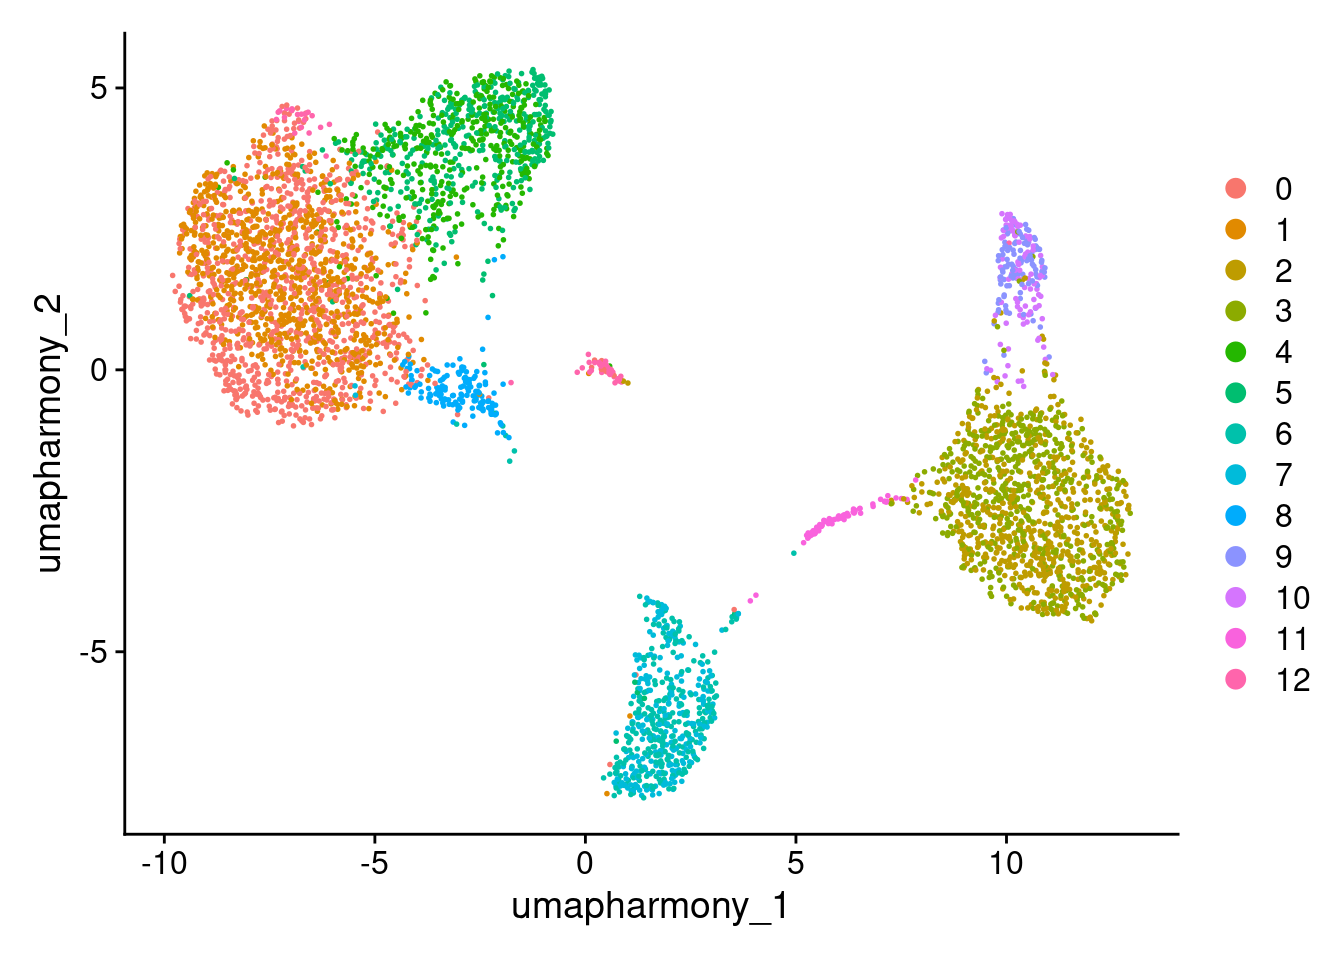
\includegraphics[keepaspectratio]{scRNAseqInR_ABACBS_2024_Doco_files/figure-latex/unnamed-chunk-22-1.pdf}}

\begin{Shaded}
\begin{Highlighting}[]
\CommentTok{\# Equivalent to}
\CommentTok{\# DimPlot(seurat\_object,reduction="umap", group.by="seurat\_clusters")}
\CommentTok{\# DimPlot(seurat\_object,reduction="umap", group.by="RNA\_snn\_res.0.5")}
\end{Highlighting}
\end{Shaded}

\begin{center}\rule{0.5\linewidth}{0.5pt}\end{center}

\subsubsection*{Challenge: Try different cluster settings}\label{challenge-try-different-cluster-settings}
\addcontentsline{toc}{subsubsection}{Challenge: Try different cluster settings}

Run \texttt{FindNeighbours} and \texttt{FindClusters} again, with a different number of dimensions or with a different resolution. Examine the resulting clusters using \texttt{DimPlot}.

To maintain the flow of this tutorial, please put the output of this exploration in a different variable, such as \texttt{seurat\_object2}!

\subsubsection*{}\label{section-11}
\addcontentsline{toc}{subsubsection}{}

\section{Choosing a cluster resolution}\label{choosing-a-cluster-resolution}

Its a good idea to try different resolutions when clustering to identify the variability of your data.

\begin{Shaded}
\begin{Highlighting}[]
\NormalTok{resolution }\OtherTok{=} \DecValTok{2}
\NormalTok{seurat\_object }\OtherTok{\textless{}{-}} \FunctionTok{FindClusters}\NormalTok{(seurat\_object, }\AttributeTok{resolution =} \FunctionTok{seq}\NormalTok{(}\FloatTok{0.1}\NormalTok{, resolution, }\FloatTok{0.1}\NormalTok{))}

\CommentTok{\# the different clustering created}
\FunctionTok{names}\NormalTok{(seurat\_object}\SpecialCharTok{@}\NormalTok{meta.data)}

\CommentTok{\# Look at cluster IDs of the first 5 cells}
\FunctionTok{head}\NormalTok{(}\FunctionTok{Idents}\NormalTok{(seurat\_object), }\DecValTok{5}\NormalTok{)}
\end{Highlighting}
\end{Shaded}

Plot a clustree to decide how many clusters you have and what resolution capture them.

\begin{Shaded}
\begin{Highlighting}[]
\FunctionTok{library}\NormalTok{(clustree)}
\CommentTok{\#\textgreater{} Loading required package: ggraph}
\CommentTok{\#\textgreater{} }
\CommentTok{\#\textgreater{} Attaching package: \textquotesingle{}ggraph\textquotesingle{}}
\CommentTok{\#\textgreater{} The following object is masked from \textquotesingle{}package:sp\textquotesingle{}:}
\CommentTok{\#\textgreater{} }
\CommentTok{\#\textgreater{}     geometry}
\FunctionTok{clustree}\NormalTok{(seurat\_object, }\AttributeTok{prefix =} \StringTok{"RNA\_snn\_res."}\NormalTok{,}\AttributeTok{show\_axis=}\ConstantTok{TRUE}\NormalTok{) }\SpecialCharTok{+} \FunctionTok{theme}\NormalTok{(}\AttributeTok{legend.key.size =} \FunctionTok{unit}\NormalTok{(}\FloatTok{0.05}\NormalTok{, }\StringTok{"cm"}\NormalTok{))}
\end{Highlighting}
\end{Shaded}

\pandocbounded{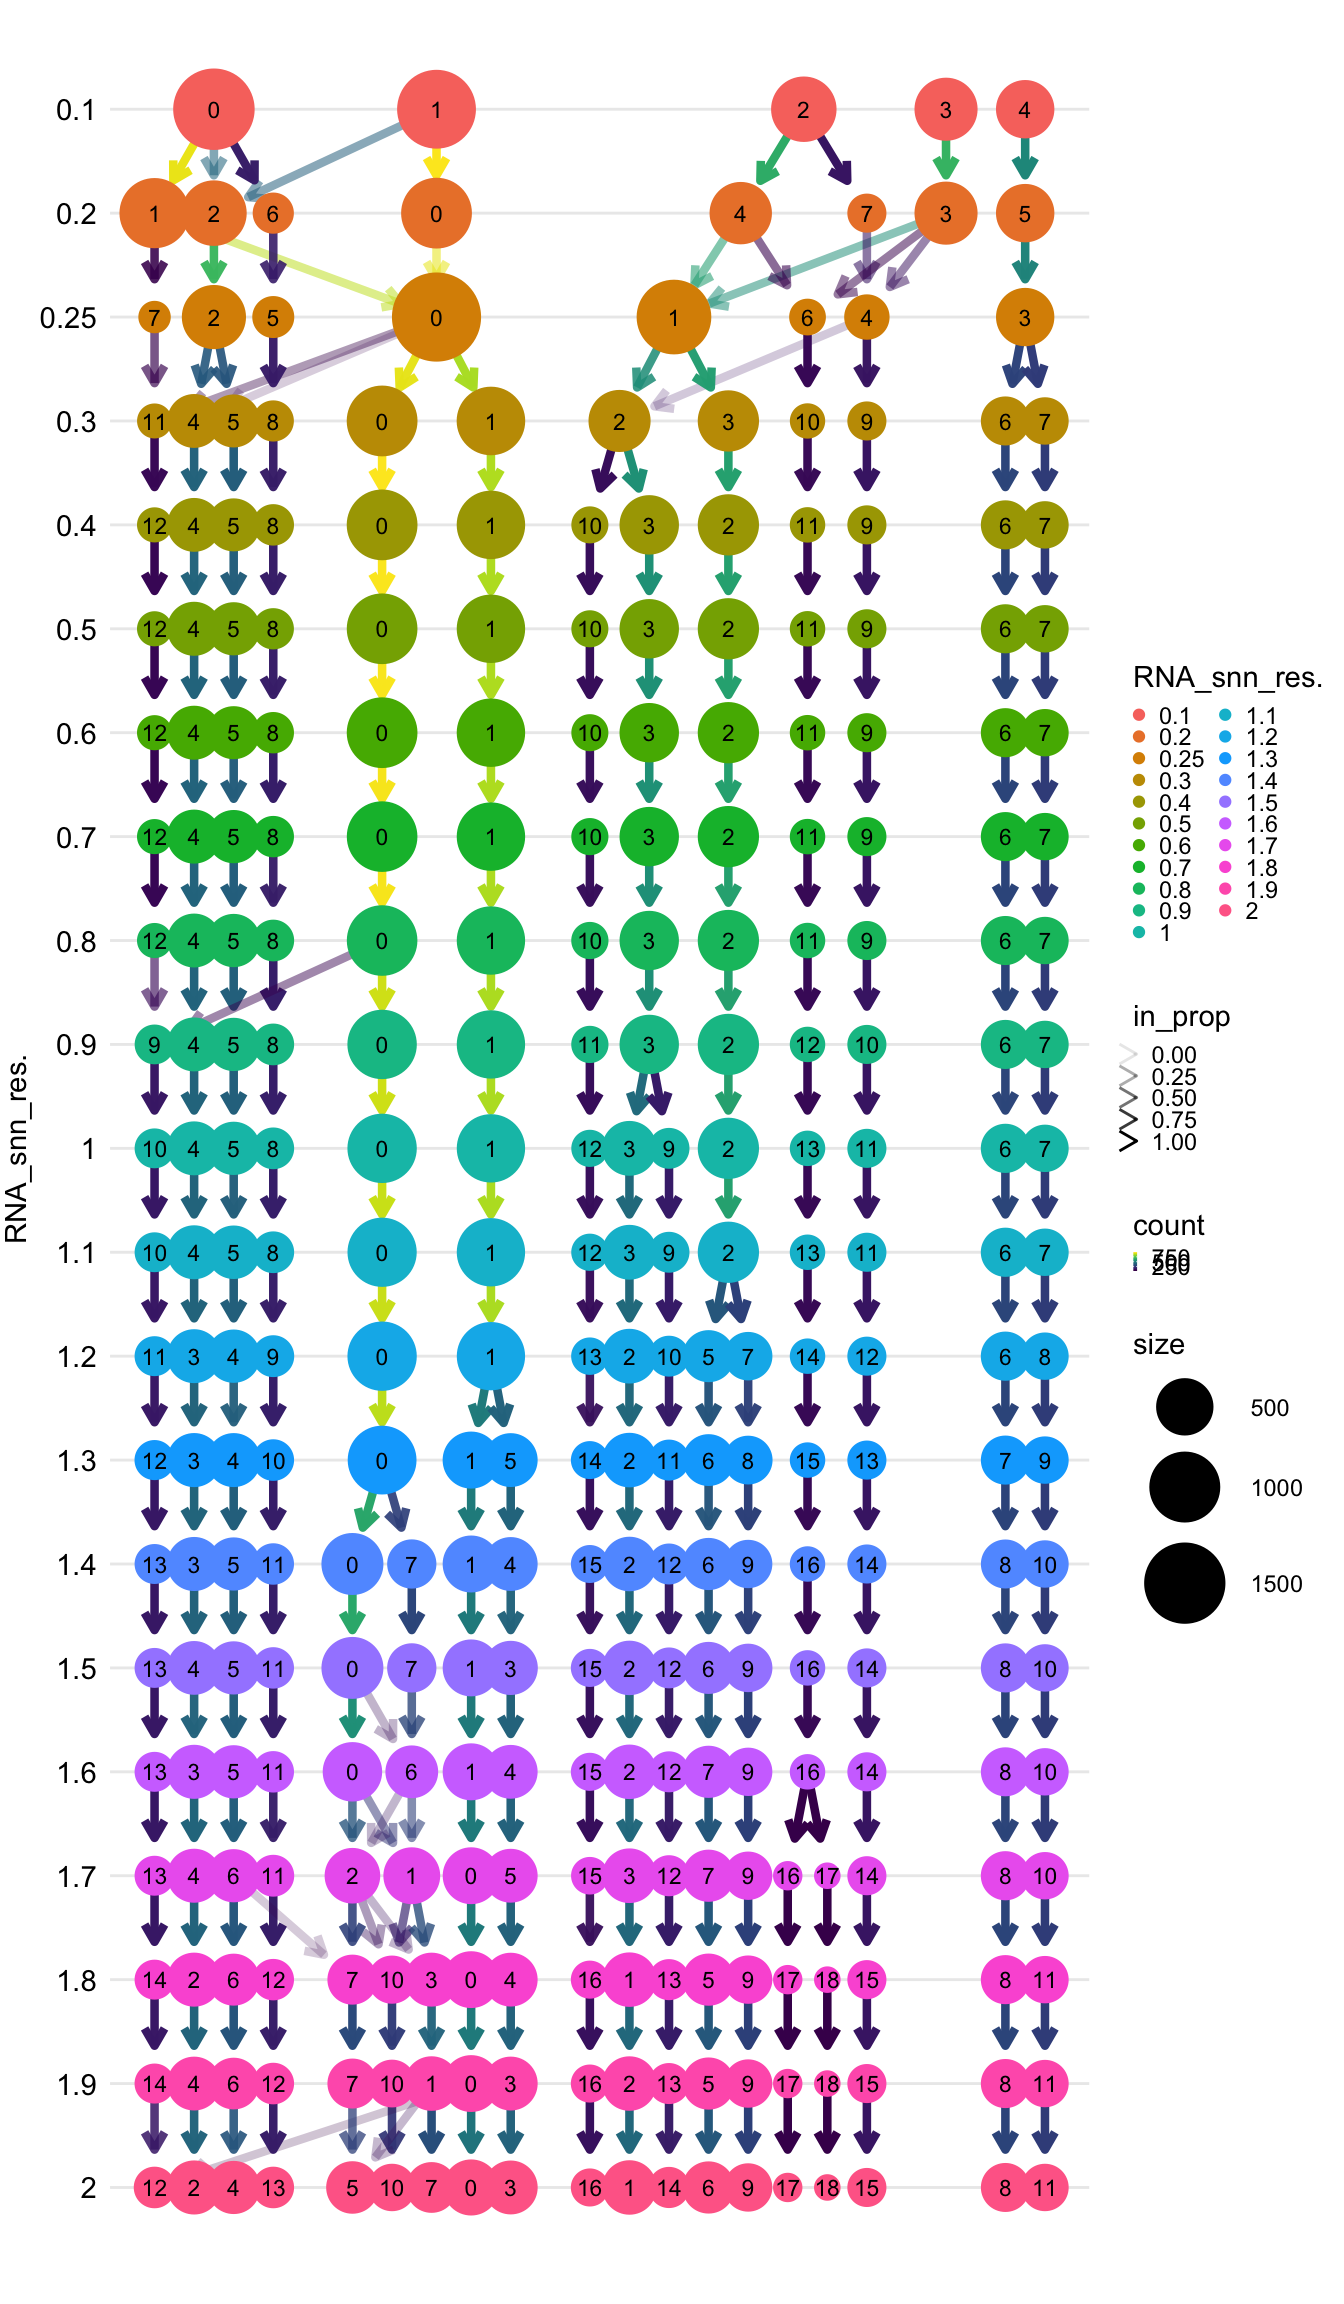
\includegraphics[keepaspectratio]{scRNAseqInR_ABACBS_2024_Doco_files/figure-latex/unnamed-chunk-24-1.pdf}}

Name cells with the corresponding cluster name at the resolution you pick. This case we are happy with 0.5.

\begin{Shaded}
\begin{Highlighting}[]
\CommentTok{\# The name of the cluster is prefixed with \textquotesingle{}RNA\_snn\_res\textquotesingle{} and the number of the resolution}
\FunctionTok{Idents}\NormalTok{(seurat\_object) }\OtherTok{\textless{}{-}}\NormalTok{ seurat\_object}\SpecialCharTok{$}\NormalTok{RNA\_snn\_res.}\FloatTok{0.5}
\end{Highlighting}
\end{Shaded}

Plot the UMAP with colored clusters with Dimplot

\begin{Shaded}
\begin{Highlighting}[]
\FunctionTok{DimPlot}\NormalTok{(seurat\_object, }\AttributeTok{reduction =} \StringTok{"umap\_harmony"}\NormalTok{, }\AttributeTok{label =} \ConstantTok{TRUE}\NormalTok{, }\AttributeTok{repel =} \ConstantTok{TRUE}\NormalTok{, }\AttributeTok{label.box =} \ConstantTok{TRUE}\NormalTok{) }\SpecialCharTok{+} \FunctionTok{NoLegend}\NormalTok{()}
\end{Highlighting}
\end{Shaded}

\pandocbounded{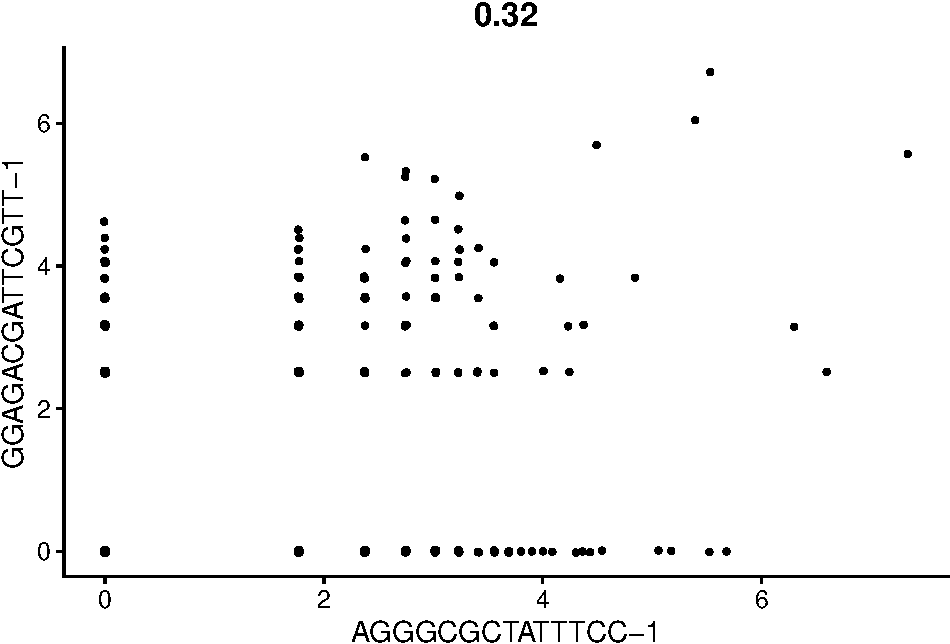
\includegraphics[keepaspectratio]{scRNAseqInR_ABACBS_2024_Doco_files/figure-latex/unnamed-chunk-26-1.pdf}}

\chapter{Cluster Markers}\label{clustermarkers}

\subsubsection*{Why do we need to do this?}\label{why-do-we-need-to-do-this-7}
\addcontentsline{toc}{subsubsection}{Why do we need to do this?}

Single cell data helps to segragate cell types. Use markers to identify cell types. warning: In this example the cell types/markers are well known and making this step easy, but in reality this step needs the experts curation.

\subsubsection*{}\label{section-12}
\addcontentsline{toc}{subsubsection}{}

\section{Finding differentially expressed features (cluster biomarkers)}\label{finding-differentially-expressed-features-cluster-biomarkers}

Seurat can help you find markers that define clusters via differential expression. By default, it identifies positive and negative markers of a single cluster (specified in \texttt{ident.1}), compared to all other cells. \texttt{FindAllMarkers()} automates this process for all clusters, but you can also test groups of clusters vs.~each other, or against all cells.

The \texttt{min.pct} argument requires a feature to be detected at a minimum percentage in either of the two groups of cells, and the thresh.test argument requires a feature to be differentially expressed (on average) by some amount between the two groups. You can set both of these to 0, but with a dramatic increase in time - since this will test a large number of features that are unlikely to be highly discriminatory. As another option to speed up these computations, \texttt{max.cells.per.ident} can be set. This will downsample each identity class to have no more cells than whatever this is set to. While there is generally going to be a loss in power, the speed increases can be significant and the most highly differentially expressed features will likely still rise to the top.

\begin{Shaded}
\begin{Highlighting}[]
\CommentTok{\# find all markers of cluster 2}
\NormalTok{cluster2.markers }\OtherTok{\textless{}{-}} \FunctionTok{FindMarkers}\NormalTok{(seurat\_object, }\AttributeTok{ident.1 =} \DecValTok{2}\NormalTok{, }\AttributeTok{min.pct =} \FloatTok{0.25}\NormalTok{)}
\FunctionTok{head}\NormalTok{(cluster2.markers, }\AttributeTok{n =} \DecValTok{5}\NormalTok{)}
\CommentTok{\#\textgreater{}      p\_val avg\_log2FC pct.1 pct.2 p\_val\_adj}
\CommentTok{\#\textgreater{} NKG7     0   5.760837 0.802 0.055         0}
\CommentTok{\#\textgreater{} CCL5     0   4.490605 0.749 0.106         0}
\CommentTok{\#\textgreater{} GNLY     0   6.161437 0.663 0.048         0}
\CommentTok{\#\textgreater{} GZMB     0   5.257738 0.652 0.037         0}
\CommentTok{\#\textgreater{} CST7     0   4.782589 0.624 0.045         0}
\CommentTok{\# find all markers distinguishing cluster 5 from clusters 0 and 3}
\NormalTok{cluster5.markers }\OtherTok{\textless{}{-}} \FunctionTok{FindMarkers}\NormalTok{(seurat\_object, }\AttributeTok{ident.1 =} \DecValTok{5}\NormalTok{, }\AttributeTok{ident.2 =} \FunctionTok{c}\NormalTok{(}\DecValTok{0}\NormalTok{, }\DecValTok{3}\NormalTok{), }\AttributeTok{min.pct =} \FloatTok{0.25}\NormalTok{)}
\FunctionTok{head}\NormalTok{(cluster5.markers, }\AttributeTok{n =} \DecValTok{5}\NormalTok{)}
\CommentTok{\#\textgreater{}               p\_val avg\_log2FC pct.1 pct.2     p\_val\_adj}
\CommentTok{\#\textgreater{} PF4   9.652092e{-}191   7.934396 0.435 0.005 3.439523e{-}186}
\CommentTok{\#\textgreater{} GNG11 5.518953e{-}171   7.336953 0.429 0.008 1.966679e{-}166}
\CommentTok{\#\textgreater{} CLU   4.848919e{-}126   8.077343 0.292 0.003 1.727912e{-}121}
\CommentTok{\#\textgreater{} PPBP  6.404717e{-}108   6.987740 0.442 0.030 2.282321e{-}103}
\CommentTok{\#\textgreater{} NCOA4  2.574636e{-}52   4.363135 0.351 0.046  9.174717e{-}48}
\CommentTok{\# find markers for every cluster compared to all remaining cells, report only the positive ones}
\NormalTok{seurat\_object.markers }\OtherTok{\textless{}{-}} \FunctionTok{FindAllMarkers}\NormalTok{(seurat\_object, }\AttributeTok{only.pos =} \ConstantTok{TRUE}\NormalTok{, }\AttributeTok{min.pct =} \FloatTok{0.25}\NormalTok{, }\AttributeTok{logfc.threshold =} \FloatTok{0.25}\NormalTok{)}
\CommentTok{\#\textgreater{} Calculating cluster 0}
\CommentTok{\#\textgreater{} Calculating cluster 1}
\CommentTok{\#\textgreater{} Calculating cluster 2}
\CommentTok{\#\textgreater{} Calculating cluster 3}
\CommentTok{\#\textgreater{} Calculating cluster 4}
\CommentTok{\#\textgreater{} Calculating cluster 5}
\CommentTok{\#\textgreater{} Calculating cluster 6}
\CommentTok{\#\textgreater{} Calculating cluster 7}
\NormalTok{seurat\_object.markers }\SpecialCharTok{\%\textgreater{}\%} \FunctionTok{group\_by}\NormalTok{(cluster) }\SpecialCharTok{\%\textgreater{}\%} \FunctionTok{slice\_max}\NormalTok{(}\AttributeTok{n =} \DecValTok{2}\NormalTok{, }\AttributeTok{order\_by =}\NormalTok{ avg\_log2FC)}
\CommentTok{\#\textgreater{} \# A tibble: 16 x 7}
\CommentTok{\#\textgreater{} \# Groups:   cluster [8]}
\CommentTok{\#\textgreater{}        p\_val avg\_log2FC pct.1 pct.2 p\_val\_adj cluster gene  }
\CommentTok{\#\textgreater{}        \textless{}dbl\textgreater{}      \textless{}dbl\textgreater{} \textless{}dbl\textgreater{} \textless{}dbl\textgreater{}     \textless{}dbl\textgreater{} \textless{}fct\textgreater{}   \textless{}chr\textgreater{} }
\CommentTok{\#\textgreater{}  1 5.85e{-}192       2.07 0.611 0.224 2.09e{-}187 0       SELL  }
\CommentTok{\#\textgreater{}  2 1.04e{-}224       2.04 0.654 0.22  3.71e{-}220 0       LTB   }
\CommentTok{\#\textgreater{}  3 7.51e{-}269       7.10 0.354 0.012 2.68e{-}264 1       CCL7  }
\CommentTok{\#\textgreater{}  4 0               7.03 0.673 0.02  0         1       S100A8}
\CommentTok{\#\textgreater{}  5 0               6.16 0.663 0.048 0         2       GNLY  }
\CommentTok{\#\textgreater{}  6 3.91e{-}259       6.12 0.333 0.011 1.39e{-}254 2       GZMA  }
\CommentTok{\#\textgreater{}  7 0               6.26 0.444 0.011 0         3       MS4A1 }
\CommentTok{\#\textgreater{}  8 0               6.07 0.658 0.019 0         3       CD79A }
\CommentTok{\#\textgreater{}  9 0               6.71 0.833 0.029 0         4       VMO1  }
\CommentTok{\#\textgreater{} 10 0               5.19 0.742 0.036 0         4       MS4A4A}
\CommentTok{\#\textgreater{} 11 7.61e{-}253       7.39 0.435 0.011 2.71e{-}248 5       PF4   }
\CommentTok{\#\textgreater{} 12 9.17e{-}110       6.53 0.442 0.042 3.27e{-}105 5       PPBP  }
\CommentTok{\#\textgreater{} 13 5.78e{-} 75       4.65 0.253 0.018 2.06e{-} 70 6       NR4A2 }
\CommentTok{\#\textgreater{} 14 2.99e{-}119       4.57 0.604 0.077 1.07e{-}114 6       HSPH1 }
\CommentTok{\#\textgreater{} 15 0               8.82 0.448 0.001 0         7       CCL22 }
\CommentTok{\#\textgreater{} 16 1.61e{-}224       8.23 0.253 0.001 5.74e{-}220 7       CALCRL}
\end{Highlighting}
\end{Shaded}

Seurat has several tests for differential expression which can be set with the test.use parameter (see our \href{de_vignette.html}{DE vignette} for details). For example, the ROC test returns the `classification power' \texttt{abs(AUC-0.5)*2} for any individual marker, ranging from 0 = random to 1 = perfect.

\begin{Shaded}
\begin{Highlighting}[]
\NormalTok{cluster0.markers }\OtherTok{\textless{}{-}} \FunctionTok{FindMarkers}\NormalTok{(seurat\_object, }\AttributeTok{ident.1 =} \DecValTok{0}\NormalTok{, }\AttributeTok{logfc.threshold =} \FloatTok{0.25}\NormalTok{, }\AttributeTok{test.use =} \StringTok{"roc"}\NormalTok{, }\AttributeTok{only.pos =} \ConstantTok{TRUE}\NormalTok{)}
\end{Highlighting}
\end{Shaded}

We include several tools for visualizing marker expression. \texttt{VlnPlot()} (shows expression probability distributions across clusters), and \texttt{FeaturePlot()} (visualizes feature expression on a tSNE or PCA plot) are our most commonly used visualizations. We also suggest exploring \texttt{RidgePlot()}, \texttt{CellScatter()}, and \texttt{DotPlot()} as additional methods to view your dataset.

\begin{Shaded}
\begin{Highlighting}[]
\FunctionTok{VlnPlot}\NormalTok{(seurat\_object, }\AttributeTok{features =} \FunctionTok{c}\NormalTok{(}\StringTok{"MS4A1"}\NormalTok{, }\StringTok{"CD79A"}\NormalTok{))}
\end{Highlighting}
\end{Shaded}

\pandocbounded{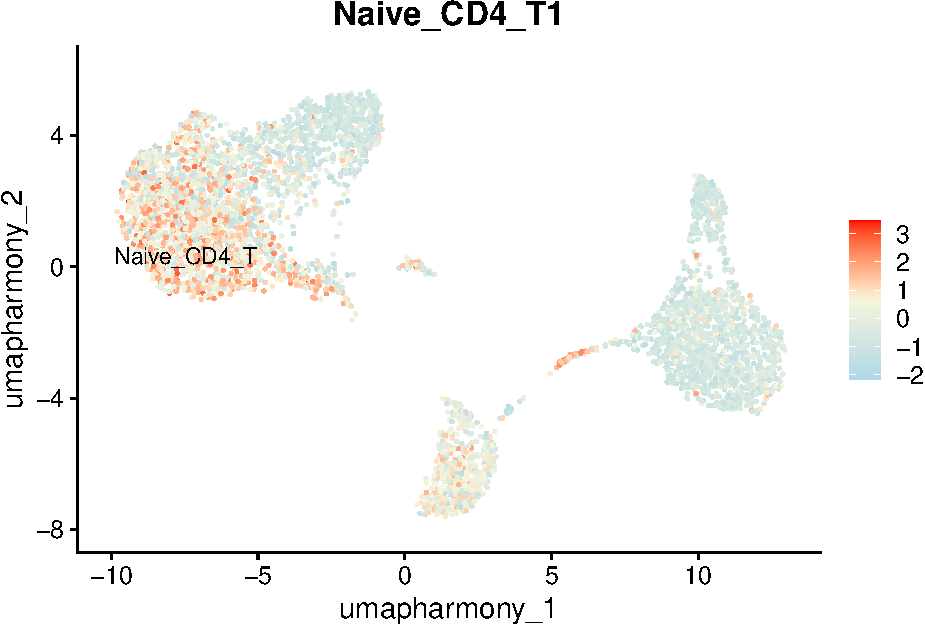
\includegraphics[keepaspectratio]{scRNAseqInR_ABACBS_2024_Doco_files/figure-latex/unnamed-chunk-28-1.pdf}}

\begin{Shaded}
\begin{Highlighting}[]
\CommentTok{\# you can plot raw counts as well}
\FunctionTok{VlnPlot}\NormalTok{(seurat\_object, }\AttributeTok{features =} \FunctionTok{c}\NormalTok{(}\StringTok{"NKG7"}\NormalTok{, }\StringTok{"PF4"}\NormalTok{), }\AttributeTok{slot =} \StringTok{\textquotesingle{}counts\textquotesingle{}}\NormalTok{, }\AttributeTok{log =} \ConstantTok{TRUE}\NormalTok{)}
\CommentTok{\#\textgreater{} Warning: The \textasciigrave{}slot\textasciigrave{} argument of \textasciigrave{}VlnPlot()\textasciigrave{} is deprecated as of}
\CommentTok{\#\textgreater{} Seurat 5.0.0.}
\CommentTok{\#\textgreater{} i Please use the \textasciigrave{}layer\textasciigrave{} argument instead.}
\CommentTok{\#\textgreater{} This warning is displayed once every 8 hours.}
\CommentTok{\#\textgreater{} Call \textasciigrave{}lifecycle::last\_lifecycle\_warnings()\textasciigrave{} to see where}
\CommentTok{\#\textgreater{} this warning was generated.}
\end{Highlighting}
\end{Shaded}

\pandocbounded{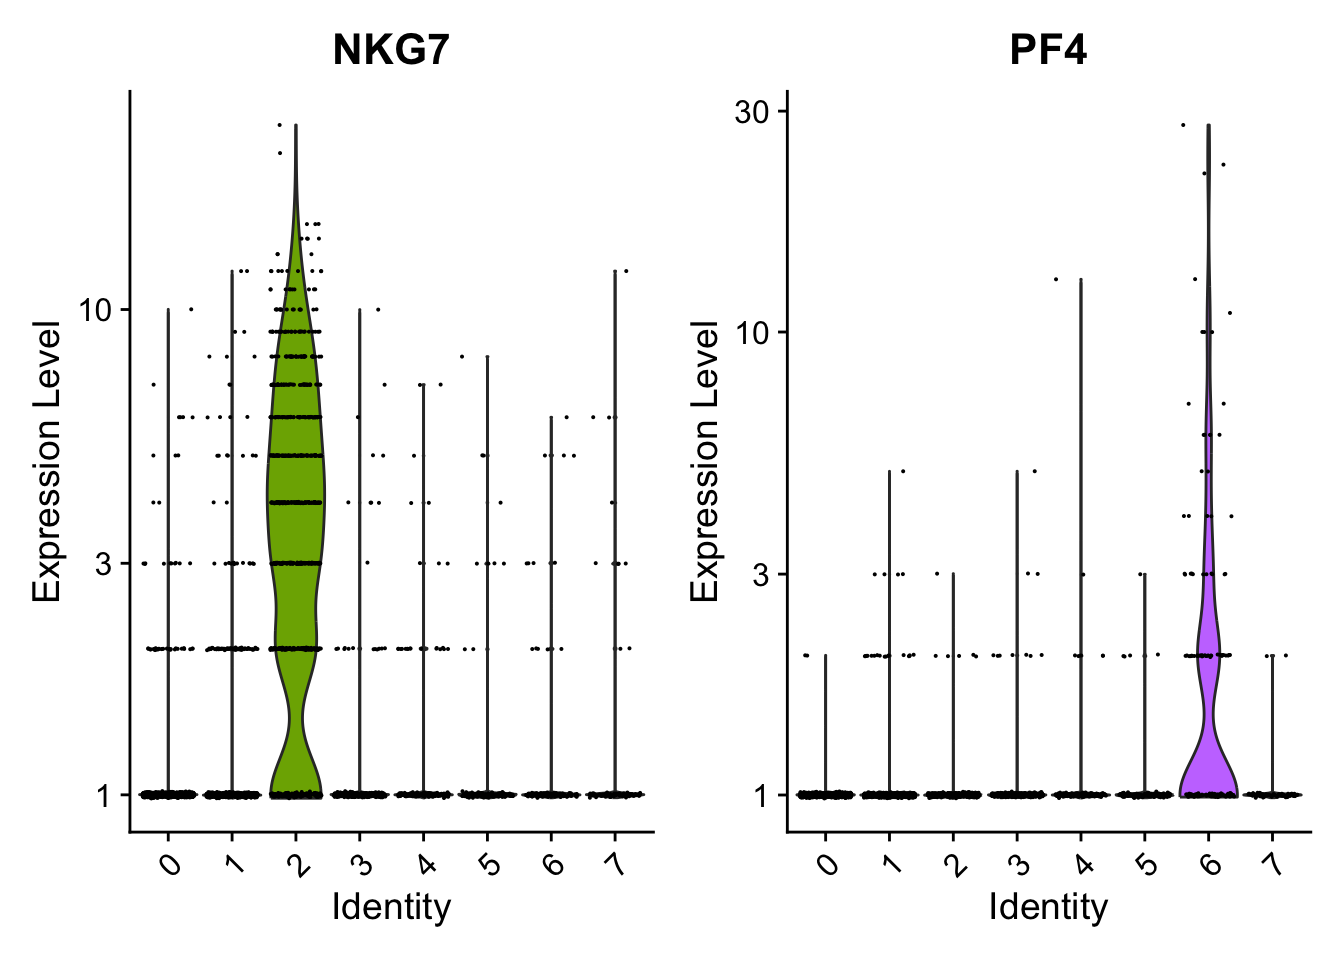
\includegraphics[keepaspectratio]{scRNAseqInR_ABACBS_2024_Doco_files/figure-latex/unnamed-chunk-28-2.pdf}}

\begin{Shaded}
\begin{Highlighting}[]
\FunctionTok{FeaturePlot}\NormalTok{(seurat\_object, }\AttributeTok{features =} \FunctionTok{c}\NormalTok{(}\StringTok{"MS4A1"}\NormalTok{, }\StringTok{"GNLY"}\NormalTok{, }\StringTok{"CD3E"}\NormalTok{, }\StringTok{"CD14"}\NormalTok{, }\StringTok{"FCER1A"}\NormalTok{))}
\end{Highlighting}
\end{Shaded}

\pandocbounded{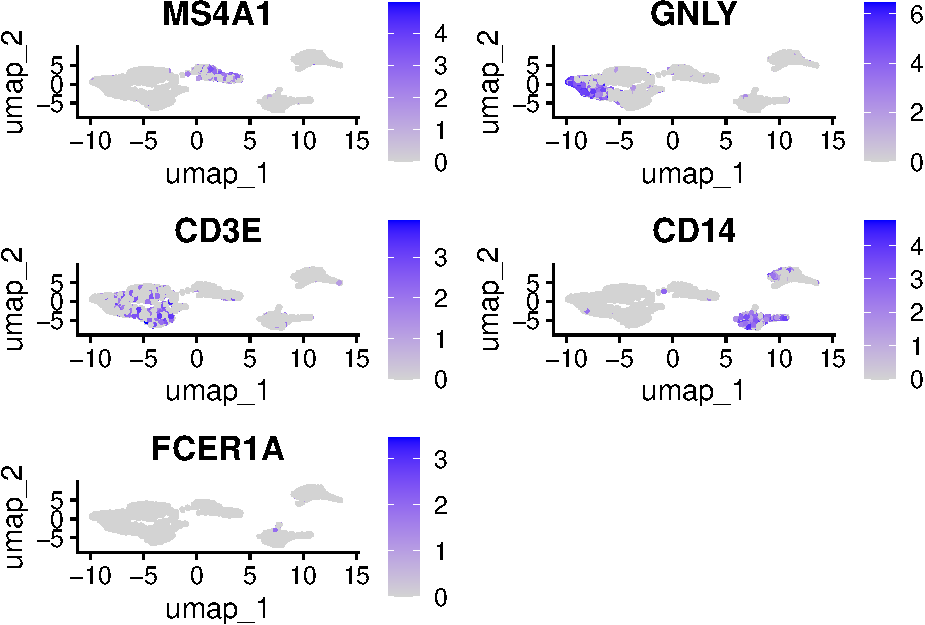
\includegraphics[keepaspectratio]{scRNAseqInR_ABACBS_2024_Doco_files/figure-latex/markerplots-1.pdf}}

\begin{Shaded}
\begin{Highlighting}[]
\FunctionTok{FeaturePlot}\NormalTok{(seurat\_object, }\AttributeTok{features =} \FunctionTok{c}\NormalTok{(}\StringTok{"FCGR3A"}\NormalTok{, }\StringTok{"LYZ"}\NormalTok{, }\StringTok{"PPBP"}\NormalTok{, }\StringTok{"CD8A"}\NormalTok{))}
\end{Highlighting}
\end{Shaded}

\pandocbounded{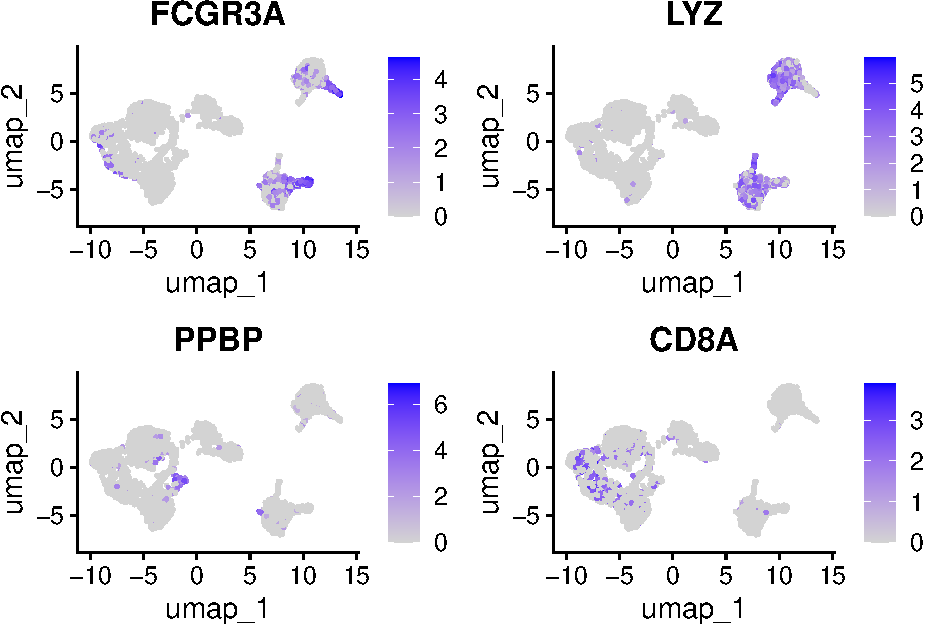
\includegraphics[keepaspectratio]{scRNAseqInR_ABACBS_2024_Doco_files/figure-latex/markerplots-2.pdf}}

\textbf{Other useful plots}

These are ridgeplots, cell scatter plots and dotplots. Replace \texttt{FeaturePlot} with the other functions.

\begin{Shaded}
\begin{Highlighting}[]
\FunctionTok{RidgePlot}\NormalTok{(seurat\_object, }\AttributeTok{features =} \FunctionTok{c}\NormalTok{(}\StringTok{"MS4A1"}\NormalTok{, }\StringTok{"GNLY"}\NormalTok{, }\StringTok{"CD3E"}\NormalTok{, }\StringTok{"CD14"}\NormalTok{, }\StringTok{"FCER1A"}\NormalTok{))}
\CommentTok{\#\textgreater{} Picking joint bandwidth of 0.0427}
\CommentTok{\#\textgreater{} Picking joint bandwidth of 0.0656}
\CommentTok{\#\textgreater{} Picking joint bandwidth of 0.0727}
\CommentTok{\#\textgreater{} Picking joint bandwidth of 0.0901}
\CommentTok{\#\textgreater{} Picking joint bandwidth of 3e{-}06}
\end{Highlighting}
\end{Shaded}

\pandocbounded{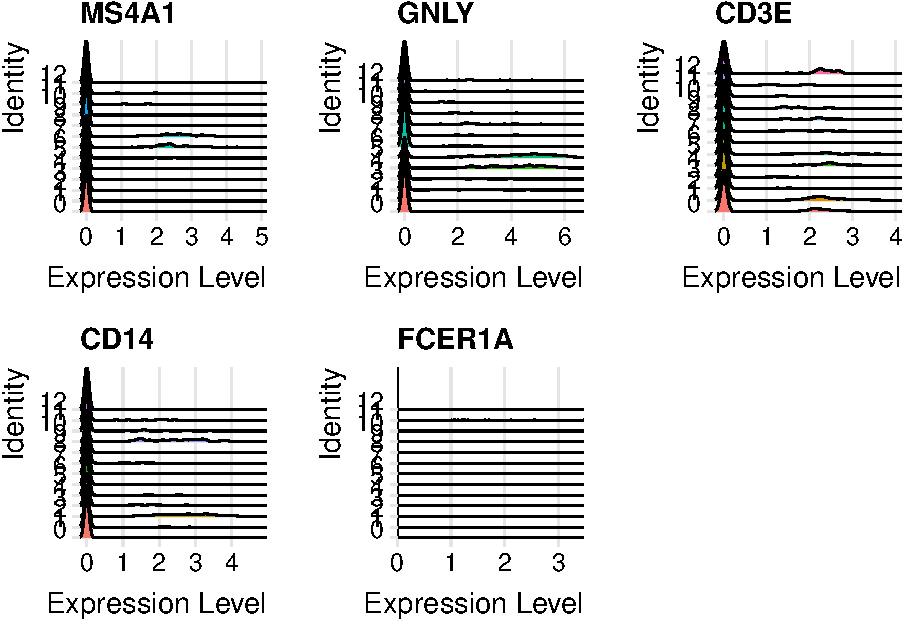
\includegraphics[keepaspectratio]{scRNAseqInR_ABACBS_2024_Doco_files/figure-latex/ridgeplots-1.pdf}}

\begin{Shaded}
\begin{Highlighting}[]
\FunctionTok{RidgePlot}\NormalTok{(seurat\_object, }\AttributeTok{features =} \FunctionTok{c}\NormalTok{(}\StringTok{"FCGR3A"}\NormalTok{, }\StringTok{"LYZ"}\NormalTok{, }\StringTok{"PPBP"}\NormalTok{, }\StringTok{"CD8A"}\NormalTok{))}
\CommentTok{\#\textgreater{} Picking joint bandwidth of 0.0547}
\CommentTok{\#\textgreater{} Picking joint bandwidth of 0.136}
\CommentTok{\#\textgreater{} Picking joint bandwidth of 0.0835}
\CommentTok{\#\textgreater{} Picking joint bandwidth of 0.0342}
\end{Highlighting}
\end{Shaded}

\pandocbounded{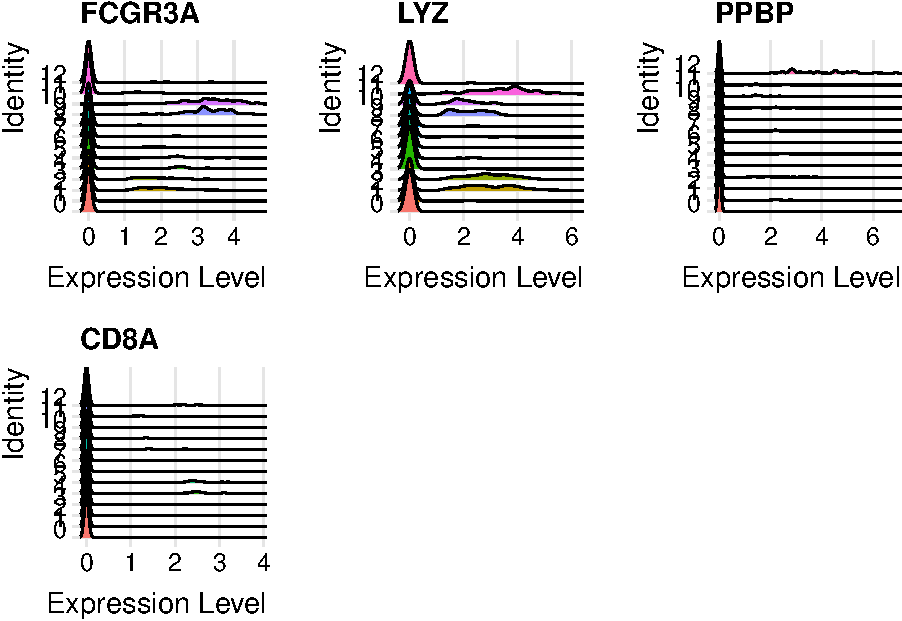
\includegraphics[keepaspectratio]{scRNAseqInR_ABACBS_2024_Doco_files/figure-latex/ridgeplots-2.pdf}}
For CellScatter plots, will need the cell id of the cells you want to look at. You can get this from the cell metadata (\texttt{seurat\_object@meta.data}).

\begin{Shaded}
\begin{Highlighting}[]
\FunctionTok{head}\NormalTok{( seurat\_object}\SpecialCharTok{@}\NormalTok{meta.data )}
\CommentTok{\#\textgreater{}                     orig.ident nCount\_RNA nFeature\_RNA  ind}
\CommentTok{\#\textgreater{} AGGGCGCTATTTCC{-}1 SeuratProject       2053          532 1256}
\CommentTok{\#\textgreater{} GGAGACGATTCGTT{-}1 SeuratProject        881          392 1256}
\CommentTok{\#\textgreater{} CACCGTTGTCGTAG{-}1 SeuratProject       3130         1005 1016}
\CommentTok{\#\textgreater{} TATCGTACACGCAT{-}1 SeuratProject       1042          549 1488}
\CommentTok{\#\textgreater{} TACGAGACCTATTC{-}1 SeuratProject       2425          777 1244}
\CommentTok{\#\textgreater{} GTACTACTCATACG{-}1 SeuratProject       3951         1064 1256}
\CommentTok{\#\textgreater{}                  stim              cell multiplets}
\CommentTok{\#\textgreater{} AGGGCGCTATTTCC{-}1 stim   CD14+ Monocytes    singlet}
\CommentTok{\#\textgreater{} GGAGACGATTCGTT{-}1 stim       CD4 T cells    singlet}
\CommentTok{\#\textgreater{} CACCGTTGTCGTAG{-}1 ctrl FCGR3A+ Monocytes    singlet}
\CommentTok{\#\textgreater{} TATCGTACACGCAT{-}1 stim           B cells    singlet}
\CommentTok{\#\textgreater{} TACGAGACCTATTC{-}1 stim       CD4 T cells    singlet}
\CommentTok{\#\textgreater{} GTACTACTCATACG{-}1 ctrl FCGR3A+ Monocytes    singlet}
\CommentTok{\#\textgreater{}                  percent.mt RNA\_snn\_res.0.5 seurat\_clusters}
\CommentTok{\#\textgreater{} AGGGCGCTATTTCC{-}1  1.6336634               1               0}
\CommentTok{\#\textgreater{} GGAGACGATTCGTT{-}1  4.8809524               5              15}
\CommentTok{\#\textgreater{} CACCGTTGTCGTAG{-}1  1.0655473               4              11}
\CommentTok{\#\textgreater{} TATCGTACACGCAT{-}1  3.0662710               3               5}
\CommentTok{\#\textgreater{} TACGAGACCTATTC{-}1  1.0837849               0               9}
\CommentTok{\#\textgreater{} GTACTACTCATACG{-}1  0.7137395               4              11}
\CommentTok{\#\textgreater{}                  pca\_clusters harmony\_clusters}
\CommentTok{\#\textgreater{} AGGGCGCTATTTCC{-}1            3                1}
\CommentTok{\#\textgreater{} GGAGACGATTCGTT{-}1            0                5}
\CommentTok{\#\textgreater{} CACCGTTGTCGTAG{-}1            9                4}
\CommentTok{\#\textgreater{} TATCGTACACGCAT{-}1            6                3}
\CommentTok{\#\textgreater{} TACGAGACCTATTC{-}1            0                0}
\CommentTok{\#\textgreater{} GTACTACTCATACG{-}1            9                4}
\CommentTok{\#\textgreater{}                  RNA\_snn\_res.0.1 RNA\_snn\_res.0.2}
\CommentTok{\#\textgreater{} AGGGCGCTATTTCC{-}1               1               1}
\CommentTok{\#\textgreater{} GGAGACGATTCGTT{-}1               0               0}
\CommentTok{\#\textgreater{} CACCGTTGTCGTAG{-}1               3               4}
\CommentTok{\#\textgreater{} TATCGTACACGCAT{-}1               2               3}
\CommentTok{\#\textgreater{} TACGAGACCTATTC{-}1               0               0}
\CommentTok{\#\textgreater{} GTACTACTCATACG{-}1               3               4}
\CommentTok{\#\textgreater{}                  RNA\_snn\_res.0.3 RNA\_snn\_res.0.4}
\CommentTok{\#\textgreater{} AGGGCGCTATTTCC{-}1               1               1}
\CommentTok{\#\textgreater{} GGAGACGATTCGTT{-}1               0               0}
\CommentTok{\#\textgreater{} CACCGTTGTCGTAG{-}1               4               4}
\CommentTok{\#\textgreater{} TATCGTACACGCAT{-}1               3               3}
\CommentTok{\#\textgreater{} TACGAGACCTATTC{-}1               0               0}
\CommentTok{\#\textgreater{} GTACTACTCATACG{-}1               4               4}
\CommentTok{\#\textgreater{}                  RNA\_snn\_res.0.6 RNA\_snn\_res.0.7}
\CommentTok{\#\textgreater{} AGGGCGCTATTTCC{-}1               1               1}
\CommentTok{\#\textgreater{} GGAGACGATTCGTT{-}1               7               6}
\CommentTok{\#\textgreater{} CACCGTTGTCGTAG{-}1               5               5}
\CommentTok{\#\textgreater{} TATCGTACACGCAT{-}1               3               3}
\CommentTok{\#\textgreater{} TACGAGACCTATTC{-}1               0               0}
\CommentTok{\#\textgreater{} GTACTACTCATACG{-}1               5               5}
\CommentTok{\#\textgreater{}                  RNA\_snn\_res.0.8 RNA\_snn\_res.0.9}
\CommentTok{\#\textgreater{} AGGGCGCTATTTCC{-}1               1               0}
\CommentTok{\#\textgreater{} GGAGACGATTCGTT{-}1               7               8}
\CommentTok{\#\textgreater{} CACCGTTGTCGTAG{-}1               6               7}
\CommentTok{\#\textgreater{} TATCGTACACGCAT{-}1               4               3}
\CommentTok{\#\textgreater{} TACGAGACCTATTC{-}1               0               1}
\CommentTok{\#\textgreater{} GTACTACTCATACG{-}1               6               7}
\CommentTok{\#\textgreater{}                  RNA\_snn\_res.1 RNA\_snn\_res.1.1}
\CommentTok{\#\textgreater{} AGGGCGCTATTTCC{-}1             1               0}
\CommentTok{\#\textgreater{} GGAGACGATTCGTT{-}1             9               9}
\CommentTok{\#\textgreater{} CACCGTTGTCGTAG{-}1             7               7}
\CommentTok{\#\textgreater{} TATCGTACACGCAT{-}1             3               3}
\CommentTok{\#\textgreater{} TACGAGACCTATTC{-}1             0               1}
\CommentTok{\#\textgreater{} GTACTACTCATACG{-}1             7               7}
\CommentTok{\#\textgreater{}                  RNA\_snn\_res.1.2 RNA\_snn\_res.1.3}
\CommentTok{\#\textgreater{} AGGGCGCTATTTCC{-}1               2               0}
\CommentTok{\#\textgreater{} GGAGACGATTCGTT{-}1               9              12}
\CommentTok{\#\textgreater{} CACCGTTGTCGTAG{-}1               7               9}
\CommentTok{\#\textgreater{} TATCGTACACGCAT{-}1               3               2}
\CommentTok{\#\textgreater{} TACGAGACCTATTC{-}1               0               8}
\CommentTok{\#\textgreater{} GTACTACTCATACG{-}1               7               9}
\CommentTok{\#\textgreater{}                  RNA\_snn\_res.1.4 RNA\_snn\_res.1.5}
\CommentTok{\#\textgreater{} AGGGCGCTATTTCC{-}1               0               0}
\CommentTok{\#\textgreater{} GGAGACGATTCGTT{-}1              14              14}
\CommentTok{\#\textgreater{} CACCGTTGTCGTAG{-}1              10              11}
\CommentTok{\#\textgreater{} TATCGTACACGCAT{-}1               2               2}
\CommentTok{\#\textgreater{} TACGAGACCTATTC{-}1               8               9}
\CommentTok{\#\textgreater{} GTACTACTCATACG{-}1              10              11}
\CommentTok{\#\textgreater{}                  RNA\_snn\_res.1.6 RNA\_snn\_res.1.7}
\CommentTok{\#\textgreater{} AGGGCGCTATTTCC{-}1               2               0}
\CommentTok{\#\textgreater{} GGAGACGATTCGTT{-}1              15              14}
\CommentTok{\#\textgreater{} CACCGTTGTCGTAG{-}1              12              11}
\CommentTok{\#\textgreater{} TATCGTACACGCAT{-}1               0               2}
\CommentTok{\#\textgreater{} TACGAGACCTATTC{-}1               9               9}
\CommentTok{\#\textgreater{} GTACTACTCATACG{-}1              12              11}
\CommentTok{\#\textgreater{}                  RNA\_snn\_res.1.8 RNA\_snn\_res.1.9}
\CommentTok{\#\textgreater{} AGGGCGCTATTTCC{-}1               0               4}
\CommentTok{\#\textgreater{} GGAGACGATTCGTT{-}1              14              16}
\CommentTok{\#\textgreater{} CACCGTTGTCGTAG{-}1              11              12}
\CommentTok{\#\textgreater{} TATCGTACACGCAT{-}1               2               0}
\CommentTok{\#\textgreater{} TACGAGACCTATTC{-}1              10               6}
\CommentTok{\#\textgreater{} GTACTACTCATACG{-}1              11              12}
\CommentTok{\#\textgreater{}                  RNA\_snn\_res.2}
\CommentTok{\#\textgreater{} AGGGCGCTATTTCC{-}1             0}
\CommentTok{\#\textgreater{} GGAGACGATTCGTT{-}1            15}
\CommentTok{\#\textgreater{} CACCGTTGTCGTAG{-}1            11}
\CommentTok{\#\textgreater{} TATCGTACACGCAT{-}1             5}
\CommentTok{\#\textgreater{} TACGAGACCTATTC{-}1             9}
\CommentTok{\#\textgreater{} GTACTACTCATACG{-}1            11}

\FunctionTok{CellScatter}\NormalTok{(seurat\_object, }\AttributeTok{cell1 =} \StringTok{"AGGGCGCTATTTCC{-}1"}\NormalTok{, }\AttributeTok{cell2 =} \StringTok{"GGAGACGATTCGTT{-}1"}\NormalTok{)}
\end{Highlighting}
\end{Shaded}

\pandocbounded{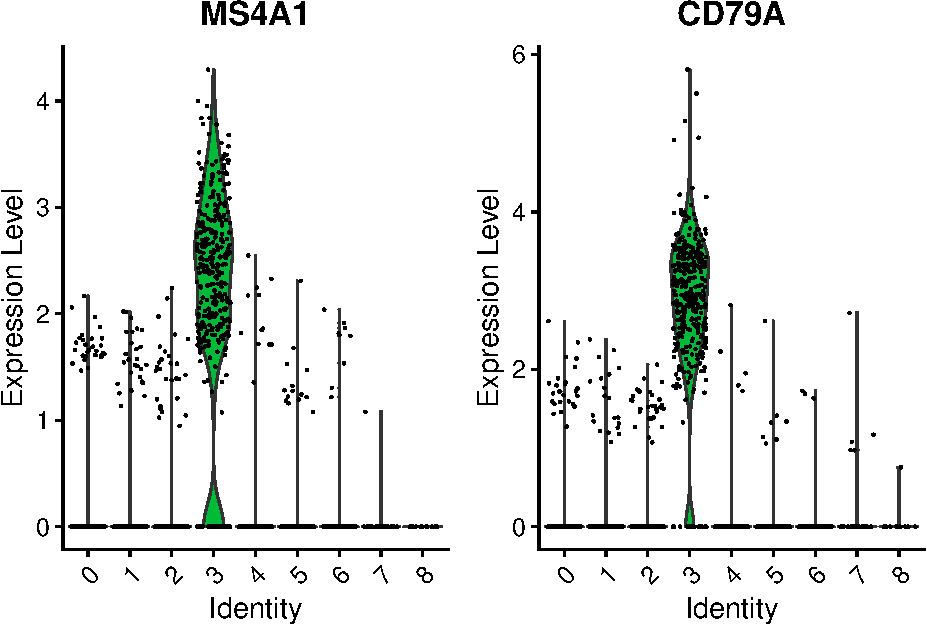
\includegraphics[keepaspectratio]{scRNAseqInR_ABACBS_2024_Doco_files/figure-latex/unnamed-chunk-29-1.pdf}}

\begin{Shaded}
\begin{Highlighting}[]

\FunctionTok{CellScatter}\NormalTok{(seurat\_object, }\AttributeTok{cell1 =} \StringTok{"GGAGACGATTCGTT{-}1"}\NormalTok{, }\AttributeTok{cell2 =} \StringTok{"TACGAGACCTATTC{-}1"}\NormalTok{)}
\end{Highlighting}
\end{Shaded}

\pandocbounded{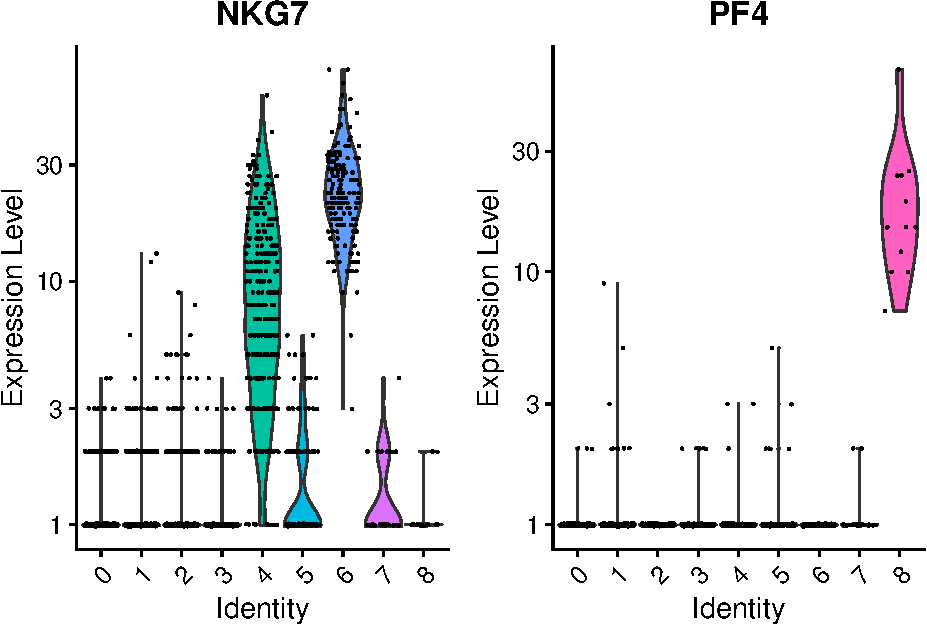
\includegraphics[keepaspectratio]{scRNAseqInR_ABACBS_2024_Doco_files/figure-latex/unnamed-chunk-29-2.pdf}}

DotPlots

\begin{Shaded}
\begin{Highlighting}[]
\FunctionTok{DotPlot}\NormalTok{(seurat\_object, }\AttributeTok{features =} \FunctionTok{c}\NormalTok{(}\StringTok{"MS4A1"}\NormalTok{, }\StringTok{"GNLY"}\NormalTok{, }\StringTok{"CD3E"}\NormalTok{, }\StringTok{"CD14"}\NormalTok{, }\StringTok{"FCER1A"}\NormalTok{, }\StringTok{"FCGR3A"}\NormalTok{, }\StringTok{"LYZ"}\NormalTok{, }\StringTok{"PPBP"}\NormalTok{, }\StringTok{"CD8A"}\NormalTok{))}
\end{Highlighting}
\end{Shaded}

\pandocbounded{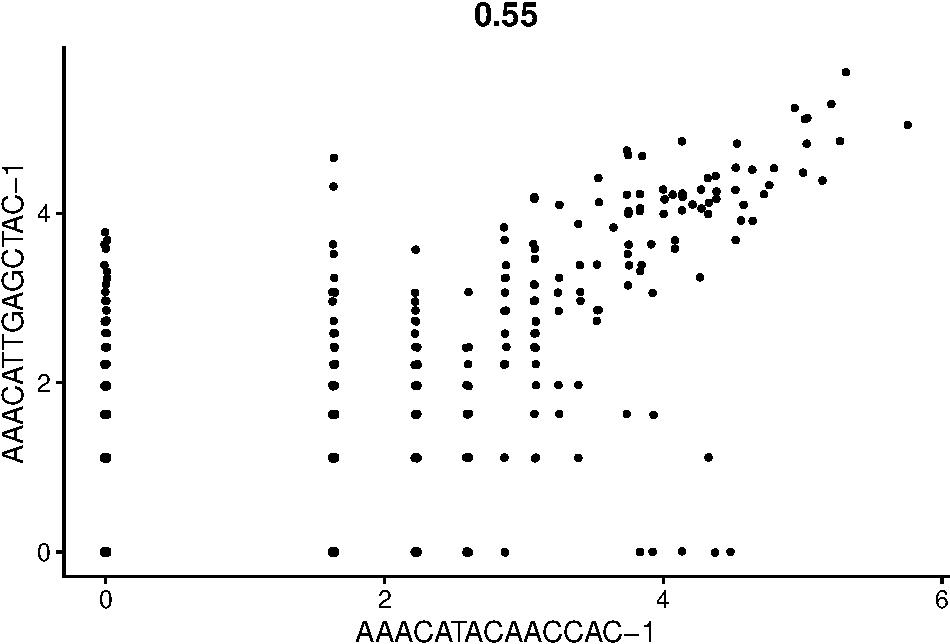
\includegraphics[keepaspectratio]{scRNAseqInR_ABACBS_2024_Doco_files/figure-latex/unnamed-chunk-30-1.pdf}}

\texttt{DoHeatmap()} generates an expression heatmap for given cells and features. In this case, we are plotting the top 10 markers (or all markers if less than 10) for each cluster.

\begin{Shaded}
\begin{Highlighting}[]
\NormalTok{maxcells}\OtherTok{=}\DecValTok{1500}
\NormalTok{top10 }\OtherTok{\textless{}{-}}\NormalTok{ seurat\_object.markers }\SpecialCharTok{\%\textgreater{}\%} \FunctionTok{group\_by}\NormalTok{(cluster) }\SpecialCharTok{\%\textgreater{}\%} \FunctionTok{top\_n}\NormalTok{(}\AttributeTok{n =} \DecValTok{10}\NormalTok{, }\AttributeTok{wt =}\NormalTok{ avg\_log2FC)}
\FunctionTok{DoHeatmap}\NormalTok{(}\FunctionTok{subset}\NormalTok{(seurat\_object, }\AttributeTok{downsample =}\NormalTok{ maxcells), }\AttributeTok{features =}\NormalTok{ top10}\SpecialCharTok{$}\NormalTok{gene) }\SpecialCharTok{+} \FunctionTok{NoLegend}\NormalTok{()}
\end{Highlighting}
\end{Shaded}

\pandocbounded{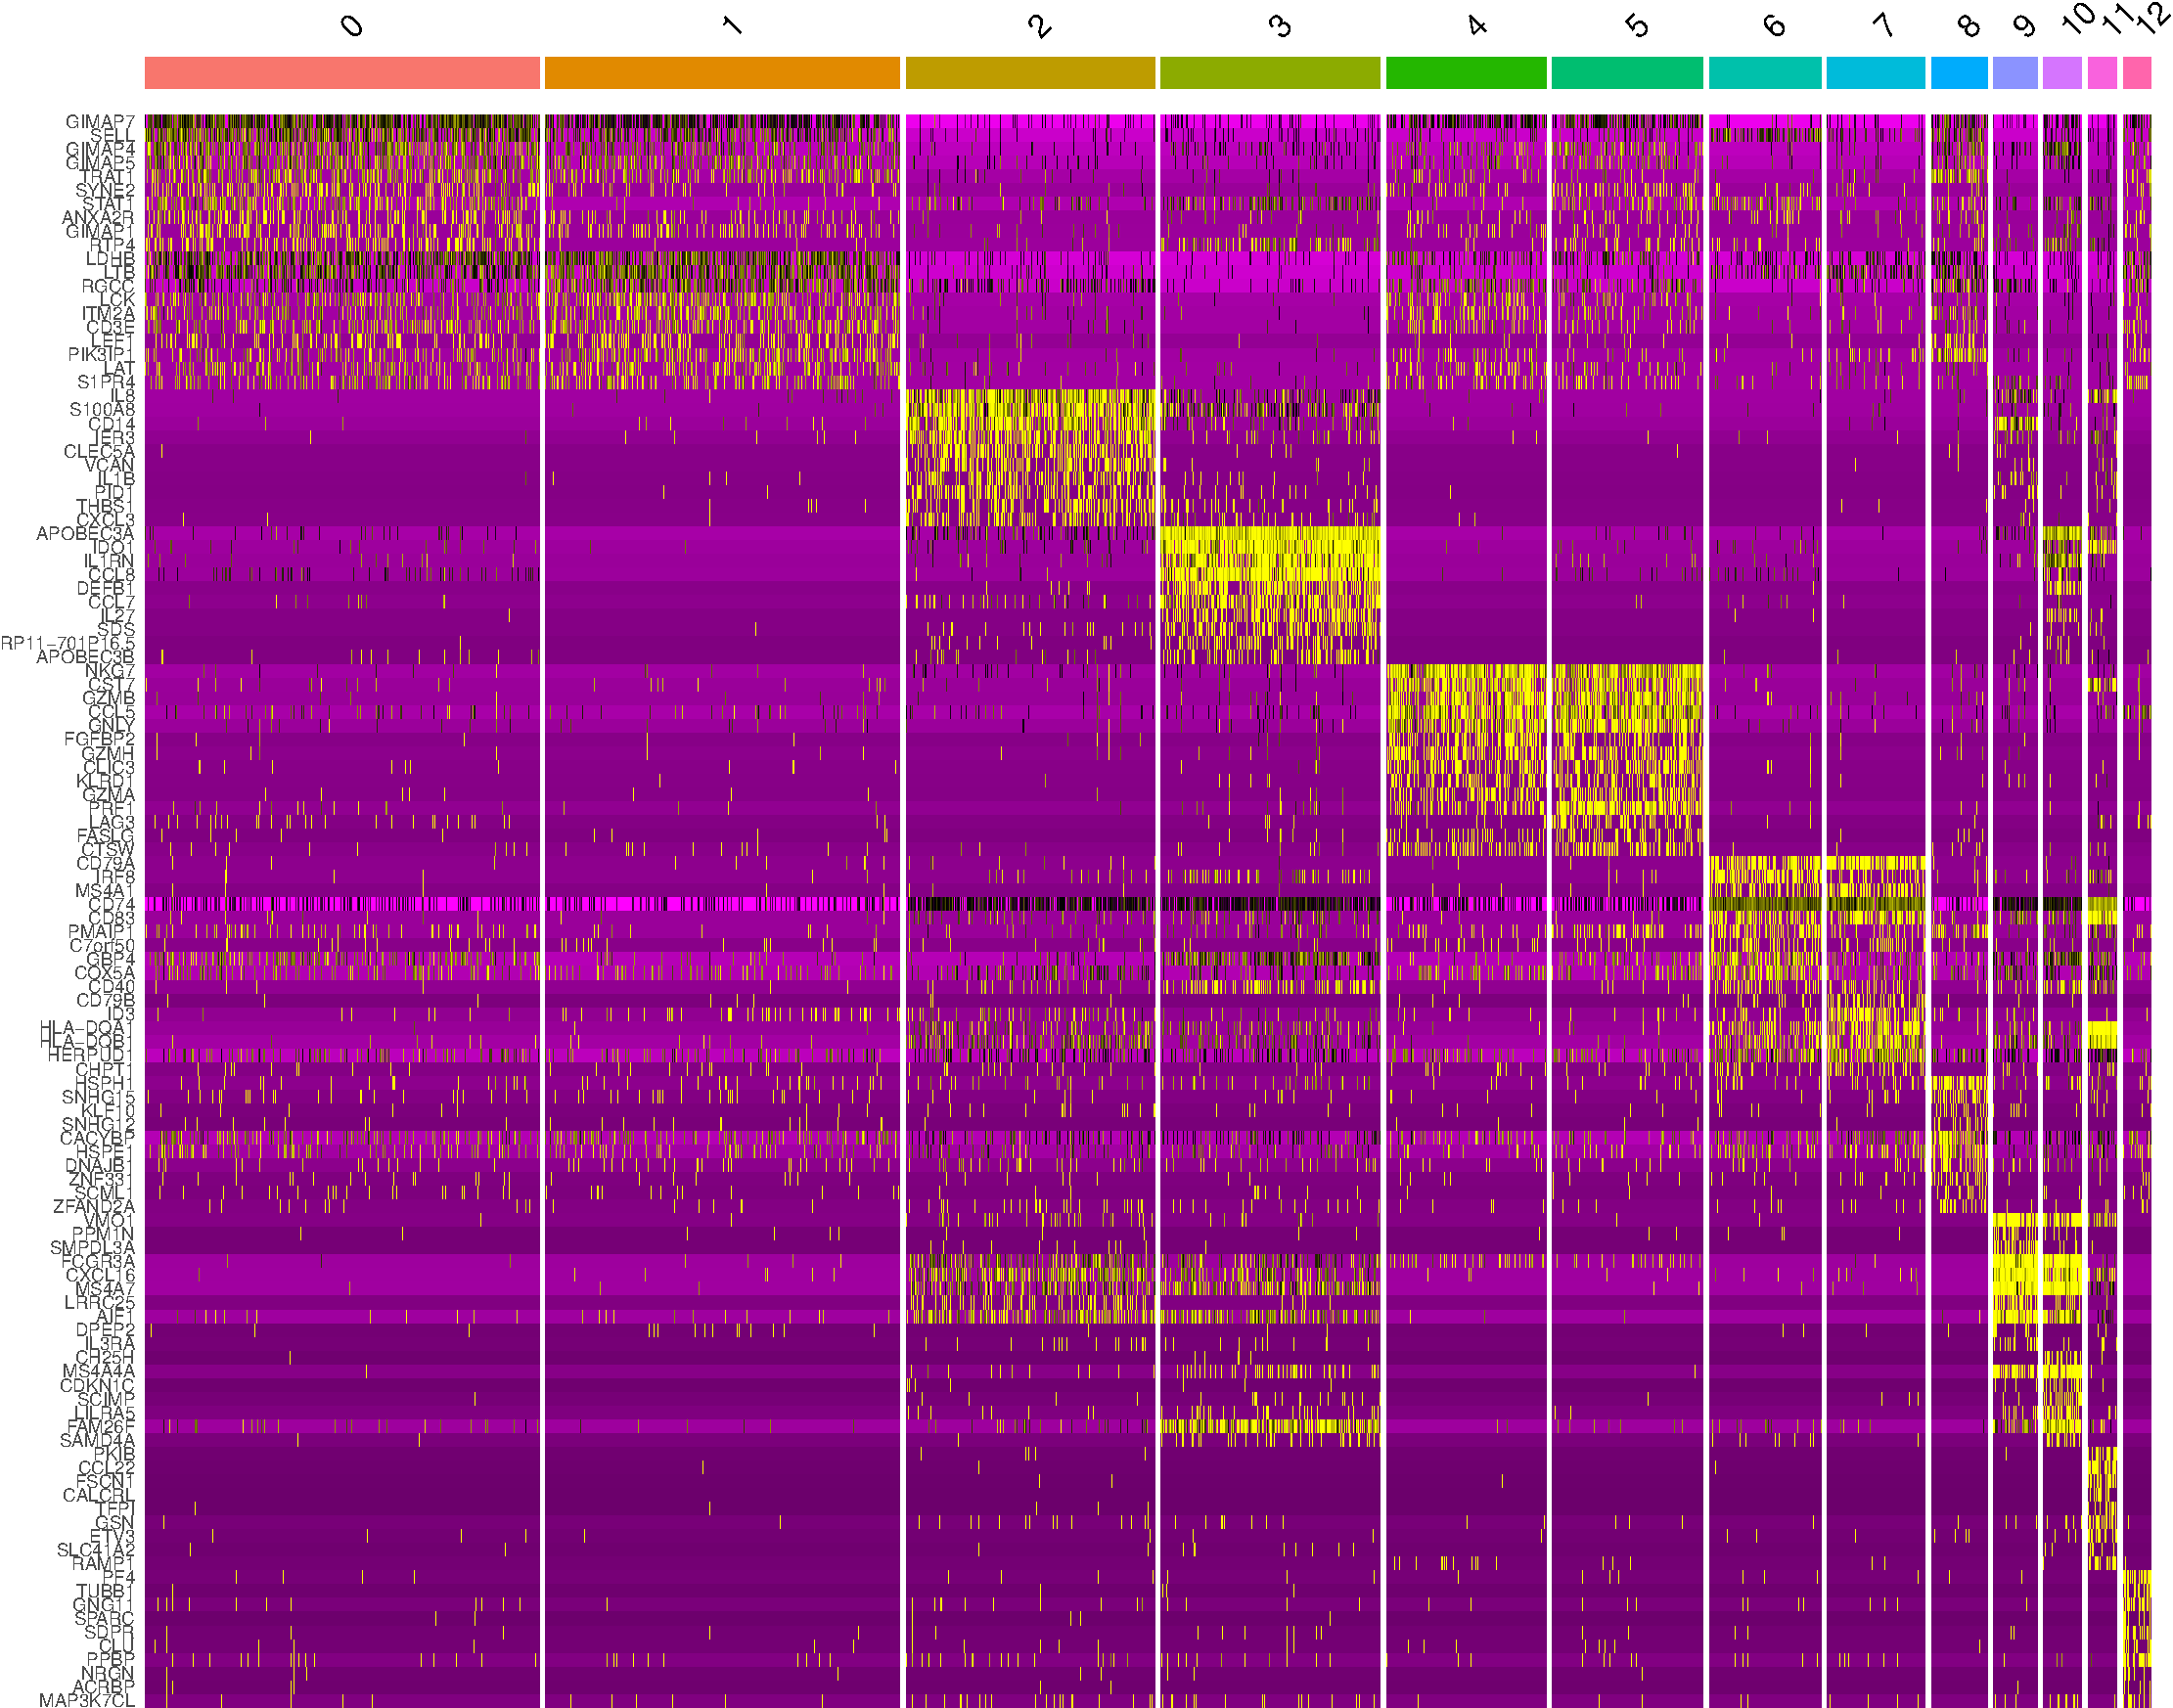
\includegraphics[keepaspectratio]{scRNAseqInR_ABACBS_2024_Doco_files/figure-latex/clusterHeatmap-1.pdf}}

\section{Use makers to label or find a cluster}\label{use-makers-to-label-or-find-a-cluster}

If you know markers for your cell types, use AddModuleScore to label them.

\begin{Shaded}
\begin{Highlighting}[]
\NormalTok{genes\_markers }\OtherTok{\textless{}{-}} \FunctionTok{list}\NormalTok{(}\AttributeTok{Naive\_CD4\_T =} \FunctionTok{c}\NormalTok{(}\StringTok{"IL7R"}\NormalTok{, }\StringTok{"CCR7"}\NormalTok{))}

\NormalTok{seurat\_object }\OtherTok{\textless{}{-}} \FunctionTok{AddModuleScore}\NormalTok{(}\AttributeTok{object =}\NormalTok{ seurat\_object, }\AttributeTok{features =}\NormalTok{ genes\_markers, }\AttributeTok{ctrl =} \DecValTok{5}\NormalTok{, }\AttributeTok{name =} \StringTok{"Naive\_CD4\_T"}\NormalTok{,}
    \AttributeTok{search =} \ConstantTok{TRUE}\NormalTok{)}


\CommentTok{\# notice the name of the cluster has a 1 at the end}
\FunctionTok{names}\NormalTok{(seurat\_object}\SpecialCharTok{@}\NormalTok{meta.data)}
\CommentTok{\#\textgreater{}  [1] "orig.ident"       "nCount\_RNA"      }
\CommentTok{\#\textgreater{}  [3] "nFeature\_RNA"     "ind"             }
\CommentTok{\#\textgreater{}  [5] "stim"             "cell"            }
\CommentTok{\#\textgreater{}  [7] "multiplets"       "percent.mt"      }
\CommentTok{\#\textgreater{}  [9] "RNA\_snn\_res.0.5"  "seurat\_clusters" }
\CommentTok{\#\textgreater{} [11] "pca\_clusters"     "harmony\_clusters"}
\CommentTok{\#\textgreater{} [13] "RNA\_snn\_res.0.1"  "RNA\_snn\_res.0.2" }
\CommentTok{\#\textgreater{} [15] "RNA\_snn\_res.0.3"  "RNA\_snn\_res.0.4" }
\CommentTok{\#\textgreater{} [17] "RNA\_snn\_res.0.6"  "RNA\_snn\_res.0.7" }
\CommentTok{\#\textgreater{} [19] "RNA\_snn\_res.0.8"  "RNA\_snn\_res.0.9" }
\CommentTok{\#\textgreater{} [21] "RNA\_snn\_res.1"    "RNA\_snn\_res.1.1" }
\CommentTok{\#\textgreater{} [23] "RNA\_snn\_res.1.2"  "RNA\_snn\_res.1.3" }
\CommentTok{\#\textgreater{} [25] "RNA\_snn\_res.1.4"  "RNA\_snn\_res.1.5" }
\CommentTok{\#\textgreater{} [27] "RNA\_snn\_res.1.6"  "RNA\_snn\_res.1.7" }
\CommentTok{\#\textgreater{} [29] "RNA\_snn\_res.1.8"  "RNA\_snn\_res.1.9" }
\CommentTok{\#\textgreater{} [31] "RNA\_snn\_res.2"    "Naive\_CD4\_T1"}

\CommentTok{\# label that cell type}
\NormalTok{seurat\_object}\SpecialCharTok{$}\NormalTok{cell\_label }\OtherTok{=} \ConstantTok{NA}
\NormalTok{seurat\_object}\SpecialCharTok{$}\NormalTok{cell\_label[seurat\_object}\SpecialCharTok{$}\NormalTok{Naive\_CD4\_T1 }\SpecialCharTok{\textgreater{}} \DecValTok{1}\NormalTok{] }\OtherTok{=} \StringTok{"Naive\_CD4\_T"}
\FunctionTok{Idents}\NormalTok{(seurat\_object) }\OtherTok{=}\NormalTok{ seurat\_object}\SpecialCharTok{$}\NormalTok{cell\_label}

\CommentTok{\# plot}
\CommentTok{\# Using a custom colour scale }
\FunctionTok{FeaturePlot}\NormalTok{(seurat\_object, }\AttributeTok{features =} \StringTok{"Naive\_CD4\_T1"}\NormalTok{, }\AttributeTok{label =} \ConstantTok{TRUE}\NormalTok{, }\AttributeTok{repel =} \ConstantTok{TRUE}\NormalTok{, }\AttributeTok{reduction =} \StringTok{"umap\_harmony"}\NormalTok{) }\SpecialCharTok{+} \FunctionTok{scale\_colour\_gradientn}\NormalTok{(}\AttributeTok{colours =} \FunctionTok{c}\NormalTok{(}\StringTok{"lightblue"}\NormalTok{,}\StringTok{"beige"}\NormalTok{,}\StringTok{"red"}\NormalTok{))}
\CommentTok{\#\textgreater{} Scale for colour is already present.}
\CommentTok{\#\textgreater{} Adding another scale for colour, which will replace the}
\CommentTok{\#\textgreater{} existing scale.}
\end{Highlighting}
\end{Shaded}

\pandocbounded{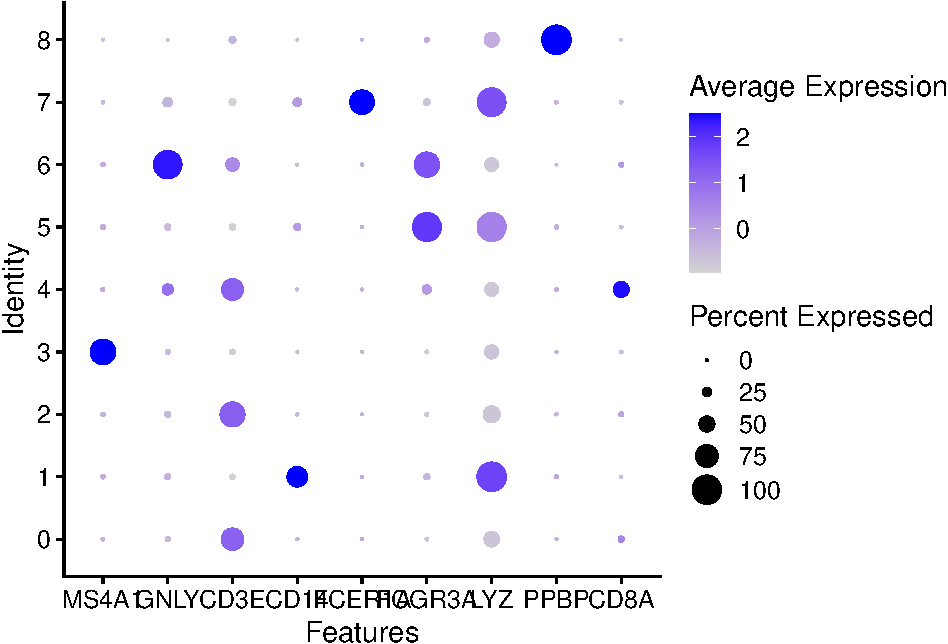
\includegraphics[keepaspectratio]{scRNAseqInR_ABACBS_2024_Doco_files/figure-latex/unnamed-chunk-31-1.pdf}}

\section{Assigning cell type identity to clusters}\label{assigning-cell-type-identity-to-clusters}

Fortunately in the case of this dataset, we can use canonical markers to easily match the unbiased clustering to known cell types:

\begin{longtable}[]{@{}ll@{}}
\toprule\noalign{}
Markers & Cell Type \\
\midrule\noalign{}
\endhead
\bottomrule\noalign{}
\endlastfoot
IL7R, CCR7 & Naive CD4+ T \\
CD14, LYZ & CD14+ Mono \\
IL7R, S100A4 & Memory CD4+ \\
MS4A1 & B \\
CD8A & CD8+ T \\
FCGR3A, MS4A7 & FCGR3A+ Mono \\
GNLY, NKG7 & NK \\
FCER1A, CST3 & DC \\
PPBP & Platelet \\
\end{longtable}

\begin{Shaded}
\begin{Highlighting}[]
\FunctionTok{DimPlot}\NormalTok{(seurat\_object,}\AttributeTok{group.by =} \StringTok{"RNA\_snn\_res.0.5"}\NormalTok{,}\AttributeTok{reduction =} \StringTok{"umap\_harmony"}\NormalTok{)}\SpecialCharTok{|}\FunctionTok{FeaturePlot}\NormalTok{(seurat\_object, }\AttributeTok{features =} \FunctionTok{c}\NormalTok{( }\StringTok{"MS4A1"}\NormalTok{),}\AttributeTok{reduction =} \StringTok{"umap\_harmony"}\NormalTok{)}
\end{Highlighting}
\end{Shaded}

\pandocbounded{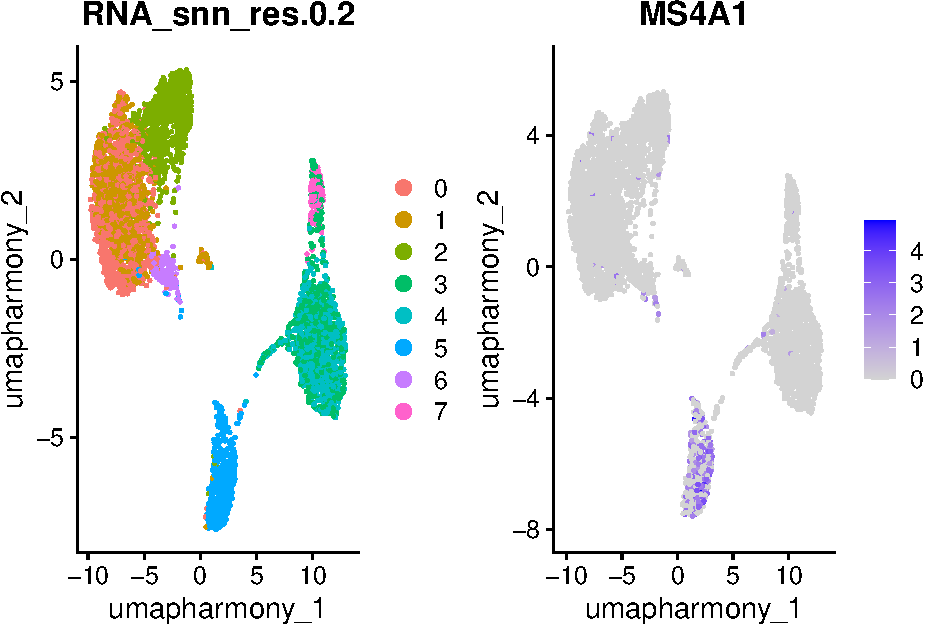
\includegraphics[keepaspectratio]{scRNAseqInR_ABACBS_2024_Doco_files/figure-latex/labelplot-1.pdf}}

\subsubsection*{Challenge: Match cluster numbers with cell labels}\label{challenge-match-cluster-numbers-with-cell-labels}
\addcontentsline{toc}{subsubsection}{Challenge: Match cluster numbers with cell labels}

Use the markers provided and the resolution 0.5 to identity the cell labels

\begin{Shaded}
\begin{Highlighting}[]
\FunctionTok{Idents}\NormalTok{(seurat\_object) }\OtherTok{\textless{}{-}}\NormalTok{ seurat\_object}\SpecialCharTok{$}\NormalTok{RNA\_snn\_res.}\FloatTok{0.5}

\CommentTok{\# This renaming list is incomplete and incorrect.}
\CommentTok{\# Fix and add to the list to fill in the cell types.}
\NormalTok{new.cluster.ids }\OtherTok{\textless{}{-}} \FunctionTok{c}\NormalTok{(}
    \StringTok{"0"} \OtherTok{=} \StringTok{"Naive CD4+ T"}\NormalTok{,}
    \StringTok{"2"} \OtherTok{=} \StringTok{"CD14+ Monocytes"}\NormalTok{,}
    \StringTok{"1"} \OtherTok{=} \StringTok{"B cells"}\NormalTok{)}

\NormalTok{seurat\_object }\OtherTok{\textless{}{-}} \FunctionTok{RenameIdents}\NormalTok{(seurat\_object, new.cluster.ids)}
\FunctionTok{DimPlot}\NormalTok{(seurat\_object, }\AttributeTok{reduction =} \StringTok{\textquotesingle{}umap\_harmony\textquotesingle{}}\NormalTok{, }\AttributeTok{label =} \ConstantTok{TRUE}\NormalTok{, }\AttributeTok{pt.size =} \FloatTok{0.5}\NormalTok{) }\SpecialCharTok{+} \FunctionTok{NoLegend}\NormalTok{()}
\end{Highlighting}
\end{Shaded}

\subsubsection*{}\label{section-13}
\addcontentsline{toc}{subsubsection}{}

\subsubsection{save the plots}\label{save-the-plots}

\begin{Shaded}
\begin{Highlighting}[]

\NormalTok{plot }\OtherTok{\textless{}{-}} \FunctionTok{DimPlot}\NormalTok{(seurat\_object, }\AttributeTok{reduction =} \StringTok{\textquotesingle{}umap\_harmony\textquotesingle{}}\NormalTok{, }\AttributeTok{label =} \ConstantTok{TRUE}\NormalTok{, }\AttributeTok{label.size =} \FloatTok{4.5}\NormalTok{) }\SpecialCharTok{+} \FunctionTok{xlab}\NormalTok{(}\StringTok{"UMAP 1"}\NormalTok{) }\SpecialCharTok{+} \FunctionTok{ylab}\NormalTok{(}\StringTok{"UMAP 2"}\NormalTok{) }\SpecialCharTok{+} 
  \FunctionTok{theme}\NormalTok{(}\AttributeTok{axis.title =} \FunctionTok{element\_text}\NormalTok{(}\AttributeTok{size =} \DecValTok{18}\NormalTok{), }\AttributeTok{legend.text =} \FunctionTok{element\_text}\NormalTok{(}\AttributeTok{size =} \DecValTok{18}\NormalTok{)) }\SpecialCharTok{+} 
  \FunctionTok{guides}\NormalTok{(}\AttributeTok{colour =} \FunctionTok{guide\_legend}\NormalTok{(}\AttributeTok{override.aes =} \FunctionTok{list}\NormalTok{(}\AttributeTok{size =} \DecValTok{10}\NormalTok{)))}
\FunctionTok{ggsave}\NormalTok{(}\AttributeTok{filename =} \StringTok{"seurat\_object3k\_umap.jpg"}\NormalTok{, }\AttributeTok{height =} \DecValTok{7}\NormalTok{, }\AttributeTok{width =} \DecValTok{12}\NormalTok{, }\AttributeTok{plot =}\NormalTok{ plot, }\AttributeTok{quality =} \DecValTok{50}\NormalTok{)}
\end{Highlighting}
\end{Shaded}

\subsubsection{save the seurat object}\label{save-the-seurat-object}

\begin{Shaded}
\begin{Highlighting}[]
\FunctionTok{saveRDS}\NormalTok{(seurat\_object, }\AttributeTok{file =} \StringTok{"seurat\_object3k\_final.rds"}\NormalTok{)}
\end{Highlighting}
\end{Shaded}

\part{Futher Analysis}\label{part-futher-analysis}

\chapter{SingleR}\label{singler}

\begin{Shaded}
\begin{Highlighting}[]
\CommentTok{\#install.packages("BiocManager")}
\CommentTok{\#BiocManager::install(c("SingleCellExperiment","SingleR","celldex"),ask=F)}
\FunctionTok{library}\NormalTok{(SingleCellExperiment)}
\FunctionTok{library}\NormalTok{(SingleR)}
\FunctionTok{library}\NormalTok{(celldex)}
\end{Highlighting}
\end{Shaded}

In this workshop we have focused on the Seurat package. However, there is another whole ecosystem of R packages for single cell analysis within Bioconductor. We won't go into any detail on these packages in this workshop, but there is good material describing the object type online : \href{https://robertamezquita.github.io/orchestratingSingleCellAnalysis/data-infrastructure.html}{OSCA}.

For now, we'll just convert our Seurat object into an object called SingleCellExperiment. Some popular packages from Bioconductor that work with this type are Slingshot, Scran, Scater.

\begin{Shaded}
\begin{Highlighting}[]
\NormalTok{sce }\OtherTok{\textless{}{-}} \FunctionTok{as.SingleCellExperiment}\NormalTok{(seurat\_object)}
\NormalTok{sce}
\CommentTok{\#\textgreater{} class: SingleCellExperiment }
\CommentTok{\#\textgreater{} dim: 35635 4877 }
\CommentTok{\#\textgreater{} metadata(0):}
\CommentTok{\#\textgreater{} assays(3): counts logcounts scaledata}
\CommentTok{\#\textgreater{} rownames(35635): MIR1302{-}10 FAM138A ... MT{-}ND6 MT{-}CYB}
\CommentTok{\#\textgreater{} rowData names(0):}
\CommentTok{\#\textgreater{} colnames(4877): AGGGCGCTATTTCC{-}1 GGAGACGATTCGTT{-}1 ...}
\CommentTok{\#\textgreater{}   ATGTTGCTAAAAGC{-}1 GATGACACTAGCGT{-}1}
\CommentTok{\#\textgreater{} colData names(34): orig.ident nCount\_RNA ...}
\CommentTok{\#\textgreater{}   cell\_label ident}
\CommentTok{\#\textgreater{} reducedDimNames(4): PCA UMAP HARMONY UMAP\_HARMONY}
\CommentTok{\#\textgreater{} mainExpName: RNA}
\CommentTok{\#\textgreater{} altExpNames(0):}
\end{Highlighting}
\end{Shaded}

We will now use a package called SingleR to label each cell. SingleR uses a reference data set of cell types with expression data to infer the best label for each cell. A convenient collection of cell type reference is in the \texttt{celldex} package which currently contains the follow sets:

\begin{Shaded}
\begin{Highlighting}[]
\FunctionTok{ls}\NormalTok{(}\StringTok{\textquotesingle{}package:celldex\textquotesingle{}}\NormalTok{)}
\CommentTok{\#\textgreater{}  [1] "BlueprintEncodeData"             }
\CommentTok{\#\textgreater{}  [2] "DatabaseImmuneCellExpressionData"}
\CommentTok{\#\textgreater{}  [3] "defineTextQuery"                 }
\CommentTok{\#\textgreater{}  [4] "fetchLatestVersion"              }
\CommentTok{\#\textgreater{}  [5] "fetchMetadata"                   }
\CommentTok{\#\textgreater{}  [6] "fetchReference"                  }
\CommentTok{\#\textgreater{}  [7] "HumanPrimaryCellAtlasData"       }
\CommentTok{\#\textgreater{}  [8] "ImmGenData"                      }
\CommentTok{\#\textgreater{}  [9] "listReferences"                  }
\CommentTok{\#\textgreater{} [10] "listVersions"                    }
\CommentTok{\#\textgreater{} [11] "MonacoImmuneData"                }
\CommentTok{\#\textgreater{} [12] "MouseRNAseqData"                 }
\CommentTok{\#\textgreater{} [13] "NovershternHematopoieticData"    }
\CommentTok{\#\textgreater{} [14] "saveReference"                   }
\CommentTok{\#\textgreater{} [15] "searchReferences"                }
\CommentTok{\#\textgreater{} [16] "surveyReferences"}
\end{Highlighting}
\end{Shaded}

In this example, we'll use the \texttt{HumanPrimaryCellAtlasData} set, which contains high-level, and fine-grained label types. Lets download the reference dataset

\begin{Shaded}
\begin{Highlighting}[]
\CommentTok{\# This too is a sce object,}
\CommentTok{\# colData is equivalent to seurat\textquotesingle{}s metadata}
\NormalTok{ref.set }\OtherTok{\textless{}{-}}\NormalTok{ celldex}\SpecialCharTok{::}\FunctionTok{HumanPrimaryCellAtlasData}\NormalTok{()}
\end{Highlighting}
\end{Shaded}

The ``main'' labels.

\begin{Shaded}
\begin{Highlighting}[]
\FunctionTok{unique}\NormalTok{(ref.set}\SpecialCharTok{$}\NormalTok{label.main)}
\CommentTok{\#\textgreater{}  [1] "DC"                   "Smooth\_muscle\_cells" }
\CommentTok{\#\textgreater{}  [3] "Epithelial\_cells"     "B\_cell"              }
\CommentTok{\#\textgreater{}  [5] "Neutrophils"          "T\_cells"             }
\CommentTok{\#\textgreater{}  [7] "Monocyte"             "Erythroblast"        }
\CommentTok{\#\textgreater{}  [9] "BM \& Prog."           "Endothelial\_cells"   }
\CommentTok{\#\textgreater{} [11] "Gametocytes"          "Neurons"             }
\CommentTok{\#\textgreater{} [13] "Keratinocytes"        "HSC\_{-}G{-}CSF"          }
\CommentTok{\#\textgreater{} [15] "Macrophage"           "NK\_cell"             }
\CommentTok{\#\textgreater{} [17] "Embryonic\_stem\_cells" "Tissue\_stem\_cells"   }
\CommentTok{\#\textgreater{} [19] "Chondrocytes"         "Osteoblasts"         }
\CommentTok{\#\textgreater{} [21] "BM"                   "Platelets"           }
\CommentTok{\#\textgreater{} [23] "Fibroblasts"          "iPS\_cells"           }
\CommentTok{\#\textgreater{} [25] "Hepatocytes"          "MSC"                 }
\CommentTok{\#\textgreater{} [27] "Neuroepithelial\_cell" "Astrocyte"           }
\CommentTok{\#\textgreater{} [29] "HSC\_CD34+"            "CMP"                 }
\CommentTok{\#\textgreater{} [31] "GMP"                  "MEP"                 }
\CommentTok{\#\textgreater{} [33] "Myelocyte"            "Pre{-}B\_cell\_CD34{-}"    }
\CommentTok{\#\textgreater{} [35] "Pro{-}B\_cell\_CD34+"     "Pro{-}Myelocyte"}
\end{Highlighting}
\end{Shaded}

An example of the types of ``fine'' labels.

\begin{Shaded}
\begin{Highlighting}[]
\FunctionTok{head}\NormalTok{(}\FunctionTok{unique}\NormalTok{(ref.set}\SpecialCharTok{$}\NormalTok{label.fine))}
\CommentTok{\#\textgreater{} [1] "DC:monocyte{-}derived:immature"       }
\CommentTok{\#\textgreater{} [2] "DC:monocyte{-}derived:Galectin{-}1"     }
\CommentTok{\#\textgreater{} [3] "DC:monocyte{-}derived:LPS"            }
\CommentTok{\#\textgreater{} [4] "DC:monocyte{-}derived"                }
\CommentTok{\#\textgreater{} [5] "Smooth\_muscle\_cells:bronchial:vit\_D"}
\CommentTok{\#\textgreater{} [6] "Smooth\_muscle\_cells:bronchial"}
\end{Highlighting}
\end{Shaded}

Now we'll label our cells using the SingleCellExperiment object, with the above reference set.

\begin{Shaded}
\begin{Highlighting}[]
\NormalTok{pred.cnts }\OtherTok{\textless{}{-}}\NormalTok{ SingleR}\SpecialCharTok{::}\FunctionTok{SingleR}\NormalTok{(}\AttributeTok{test =}\NormalTok{ sce, }\AttributeTok{ref =}\NormalTok{ ref.set, }\AttributeTok{labels =}\NormalTok{ ref.set}\SpecialCharTok{$}\NormalTok{label.main)}
\end{Highlighting}
\end{Shaded}

Keep any types that have more than 10 cells to the label, and put those labels back on our Seurat object and plot our on our umap.

\begin{Shaded}
\begin{Highlighting}[]
\NormalTok{lbls.keep }\OtherTok{\textless{}{-}} \FunctionTok{table}\NormalTok{(pred.cnts}\SpecialCharTok{$}\NormalTok{labels)}\SpecialCharTok{\textgreater{}}\DecValTok{10}
\NormalTok{seurat\_object}\SpecialCharTok{$}\NormalTok{SingleR.labels }\OtherTok{\textless{}{-}} \FunctionTok{ifelse}\NormalTok{(lbls.keep[pred.cnts}\SpecialCharTok{$}\NormalTok{labels], pred.cnts}\SpecialCharTok{$}\NormalTok{labels, }\StringTok{\textquotesingle{}Other\textquotesingle{}}\NormalTok{)}
\FunctionTok{DimPlot}\NormalTok{(seurat\_object, }\AttributeTok{reduction=}\StringTok{\textquotesingle{}umap\_harmony\textquotesingle{}}\NormalTok{, }\AttributeTok{group.by=}\StringTok{\textquotesingle{}SingleR.labels\textquotesingle{}}\NormalTok{)}
\end{Highlighting}
\end{Shaded}

\pandocbounded{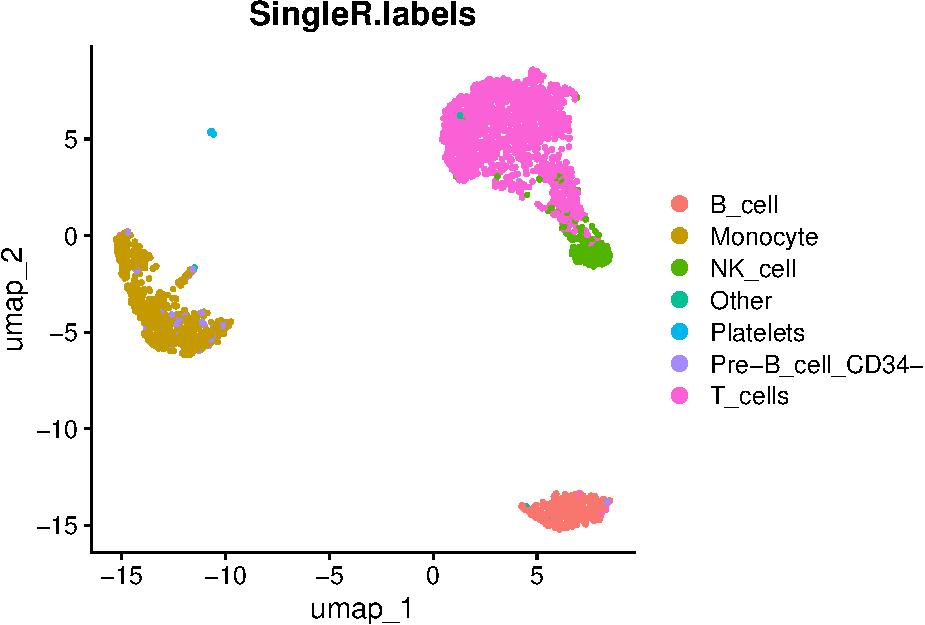
\includegraphics[keepaspectratio]{scRNAseqInR_ABACBS_2024_Doco_files/figure-latex/unnamed-chunk-41-1.pdf}}

Compare cell labels by different annotation methods:

\begin{Shaded}
\begin{Highlighting}[]
\FunctionTok{DimPlot}\NormalTok{(seurat\_object,}\AttributeTok{group.by =} \StringTok{"RNA\_snn\_res.0.5"}\NormalTok{,}\AttributeTok{reduction =} \StringTok{"umap\_harmony"}\NormalTok{)}
\end{Highlighting}
\end{Shaded}

\pandocbounded{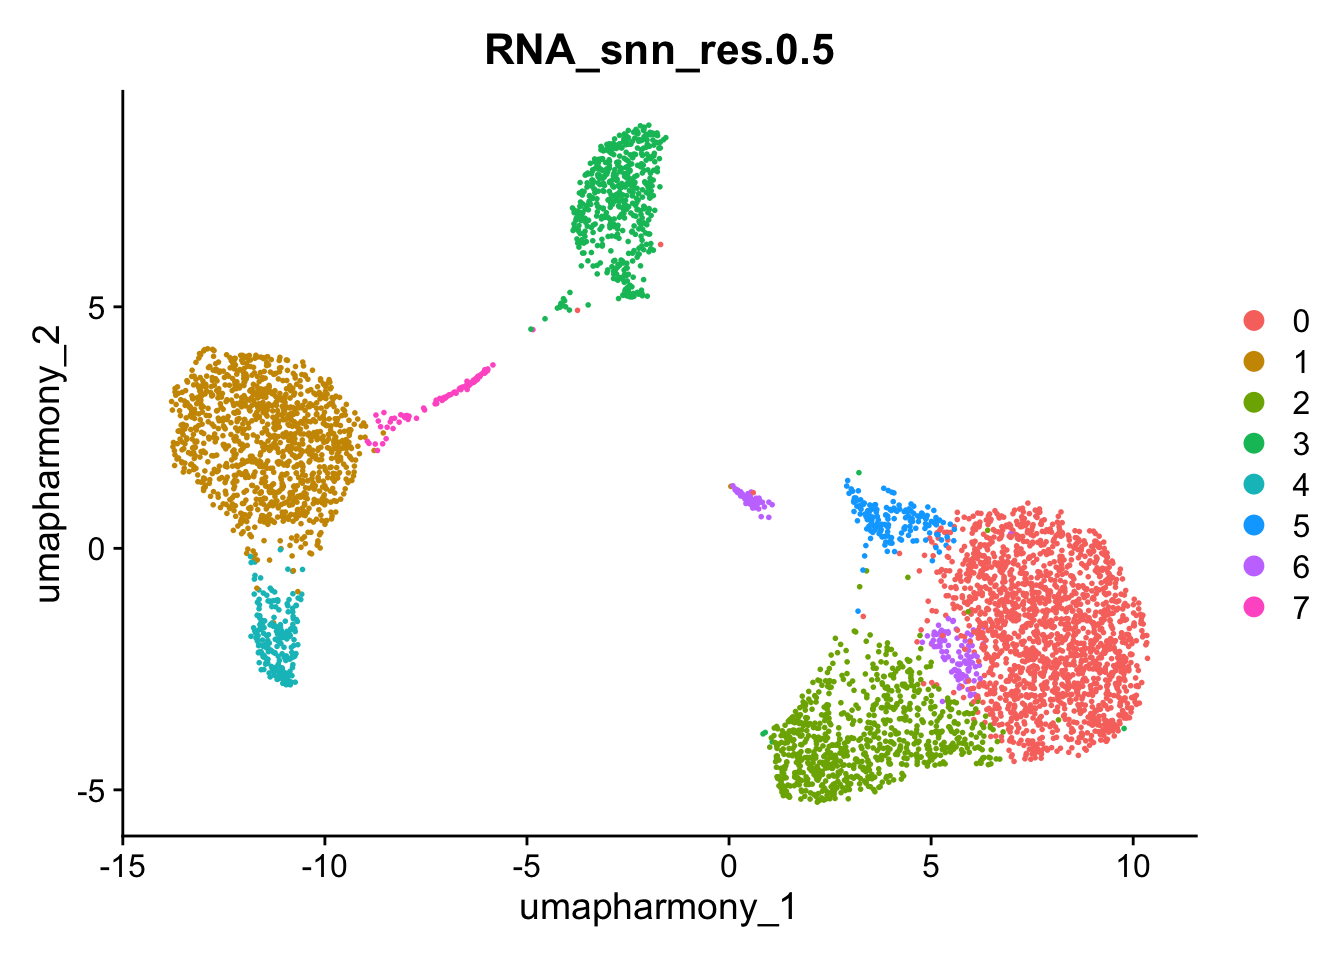
\includegraphics[keepaspectratio]{scRNAseqInR_ABACBS_2024_Doco_files/figure-latex/unnamed-chunk-42-1.pdf}}

\begin{Shaded}
\begin{Highlighting}[]

\FunctionTok{DimPlot}\NormalTok{(seurat\_object,}\AttributeTok{group.by =} \StringTok{"cell"}\NormalTok{,}\AttributeTok{reduction =} \StringTok{"umap\_harmony"}\NormalTok{)}
\end{Highlighting}
\end{Shaded}

\pandocbounded{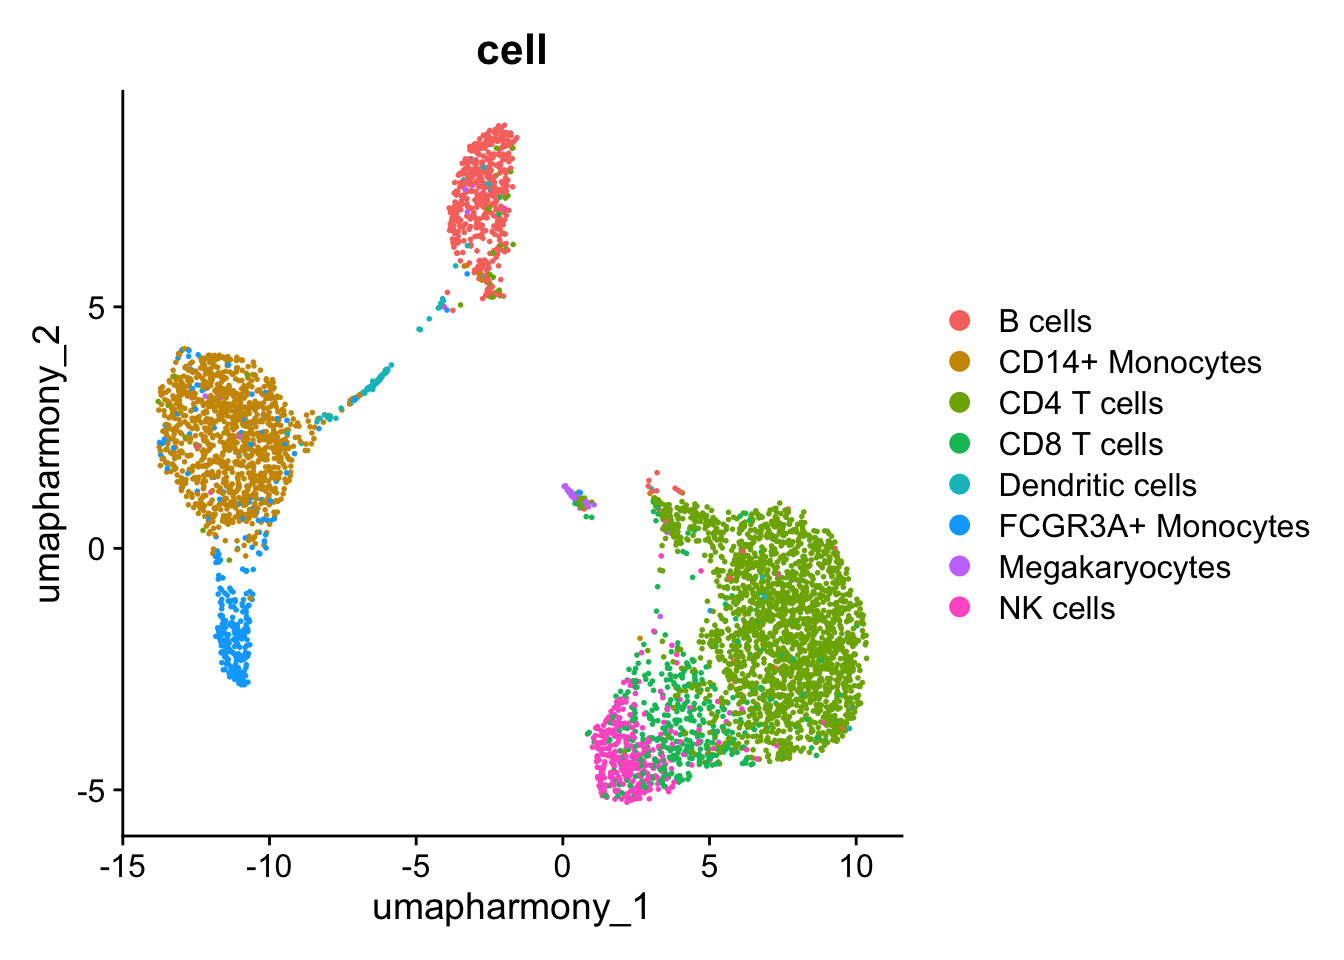
\includegraphics[keepaspectratio]{scRNAseqInR_ABACBS_2024_Doco_files/figure-latex/unnamed-chunk-42-2.pdf}}

\chapter{Differential Expression}\label{de2}

\href{https://docs.google.com/presentation/d/1iTfkc2KgGy3d6yT9zCALZzk993pWwT9D/edit\#slide=id.p1}{Slides}

There are many different methods for calculating differential expression between groups in scRNAseq data. There are a number of review papers worth consulting on this topic.

There is the \href{https://satijalab.org/seurat/archive/v3.1/de_vignette.html}{Seurat differential expression Vignette} which walks through the variety implemented in Seurat.

There is also a good discussion of useing \href{http://bioconductor.org/books/3.15/OSCA.multisample/multi-sample-comparisons.html\#creating-pseudo-bulk-samples}{pseudobulk approaches} which is worth checking out if youre planning differential expression analyses.

\begin{Shaded}
\begin{Highlighting}[]
\FunctionTok{head}\NormalTok{(seurat\_object}\SpecialCharTok{@}\NormalTok{meta.data)}
\CommentTok{\#\textgreater{}                     orig.ident nCount\_RNA nFeature\_RNA  ind}
\CommentTok{\#\textgreater{} AGGGCGCTATTTCC{-}1 SeuratProject       2053          532 1256}
\CommentTok{\#\textgreater{} GGAGACGATTCGTT{-}1 SeuratProject        881          392 1256}
\CommentTok{\#\textgreater{} CACCGTTGTCGTAG{-}1 SeuratProject       3130         1005 1016}
\CommentTok{\#\textgreater{} TATCGTACACGCAT{-}1 SeuratProject       1042          549 1488}
\CommentTok{\#\textgreater{} TACGAGACCTATTC{-}1 SeuratProject       2425          777 1244}
\CommentTok{\#\textgreater{} GTACTACTCATACG{-}1 SeuratProject       3951         1064 1256}
\CommentTok{\#\textgreater{}                  stim              cell multiplets}
\CommentTok{\#\textgreater{} AGGGCGCTATTTCC{-}1 stim   CD14+ Monocytes    singlet}
\CommentTok{\#\textgreater{} GGAGACGATTCGTT{-}1 stim       CD4 T cells    singlet}
\CommentTok{\#\textgreater{} CACCGTTGTCGTAG{-}1 ctrl FCGR3A+ Monocytes    singlet}
\CommentTok{\#\textgreater{} TATCGTACACGCAT{-}1 stim           B cells    singlet}
\CommentTok{\#\textgreater{} TACGAGACCTATTC{-}1 stim       CD4 T cells    singlet}
\CommentTok{\#\textgreater{} GTACTACTCATACG{-}1 ctrl FCGR3A+ Monocytes    singlet}
\CommentTok{\#\textgreater{}                  percent.mt RNA\_snn\_res.0.5 seurat\_clusters}
\CommentTok{\#\textgreater{} AGGGCGCTATTTCC{-}1  1.6336634               1               0}
\CommentTok{\#\textgreater{} GGAGACGATTCGTT{-}1  4.8809524               5              15}
\CommentTok{\#\textgreater{} CACCGTTGTCGTAG{-}1  1.0655473               4              11}
\CommentTok{\#\textgreater{} TATCGTACACGCAT{-}1  3.0662710               3               5}
\CommentTok{\#\textgreater{} TACGAGACCTATTC{-}1  1.0837849               0               9}
\CommentTok{\#\textgreater{} GTACTACTCATACG{-}1  0.7137395               4              11}
\CommentTok{\#\textgreater{}                  pca\_clusters harmony\_clusters}
\CommentTok{\#\textgreater{} AGGGCGCTATTTCC{-}1            3                1}
\CommentTok{\#\textgreater{} GGAGACGATTCGTT{-}1            0                5}
\CommentTok{\#\textgreater{} CACCGTTGTCGTAG{-}1            9                4}
\CommentTok{\#\textgreater{} TATCGTACACGCAT{-}1            6                3}
\CommentTok{\#\textgreater{} TACGAGACCTATTC{-}1            0                0}
\CommentTok{\#\textgreater{} GTACTACTCATACG{-}1            9                4}
\CommentTok{\#\textgreater{}                  RNA\_snn\_res.0.1 RNA\_snn\_res.0.2}
\CommentTok{\#\textgreater{} AGGGCGCTATTTCC{-}1               1               1}
\CommentTok{\#\textgreater{} GGAGACGATTCGTT{-}1               0               0}
\CommentTok{\#\textgreater{} CACCGTTGTCGTAG{-}1               3               4}
\CommentTok{\#\textgreater{} TATCGTACACGCAT{-}1               2               3}
\CommentTok{\#\textgreater{} TACGAGACCTATTC{-}1               0               0}
\CommentTok{\#\textgreater{} GTACTACTCATACG{-}1               3               4}
\CommentTok{\#\textgreater{}                  RNA\_snn\_res.0.3 RNA\_snn\_res.0.4}
\CommentTok{\#\textgreater{} AGGGCGCTATTTCC{-}1               1               1}
\CommentTok{\#\textgreater{} GGAGACGATTCGTT{-}1               0               0}
\CommentTok{\#\textgreater{} CACCGTTGTCGTAG{-}1               4               4}
\CommentTok{\#\textgreater{} TATCGTACACGCAT{-}1               3               3}
\CommentTok{\#\textgreater{} TACGAGACCTATTC{-}1               0               0}
\CommentTok{\#\textgreater{} GTACTACTCATACG{-}1               4               4}
\CommentTok{\#\textgreater{}                  RNA\_snn\_res.0.6 RNA\_snn\_res.0.7}
\CommentTok{\#\textgreater{} AGGGCGCTATTTCC{-}1               1               1}
\CommentTok{\#\textgreater{} GGAGACGATTCGTT{-}1               7               6}
\CommentTok{\#\textgreater{} CACCGTTGTCGTAG{-}1               5               5}
\CommentTok{\#\textgreater{} TATCGTACACGCAT{-}1               3               3}
\CommentTok{\#\textgreater{} TACGAGACCTATTC{-}1               0               0}
\CommentTok{\#\textgreater{} GTACTACTCATACG{-}1               5               5}
\CommentTok{\#\textgreater{}                  RNA\_snn\_res.0.8 RNA\_snn\_res.0.9}
\CommentTok{\#\textgreater{} AGGGCGCTATTTCC{-}1               1               0}
\CommentTok{\#\textgreater{} GGAGACGATTCGTT{-}1               7               8}
\CommentTok{\#\textgreater{} CACCGTTGTCGTAG{-}1               6               7}
\CommentTok{\#\textgreater{} TATCGTACACGCAT{-}1               4               3}
\CommentTok{\#\textgreater{} TACGAGACCTATTC{-}1               0               1}
\CommentTok{\#\textgreater{} GTACTACTCATACG{-}1               6               7}
\CommentTok{\#\textgreater{}                  RNA\_snn\_res.1 RNA\_snn\_res.1.1}
\CommentTok{\#\textgreater{} AGGGCGCTATTTCC{-}1             1               0}
\CommentTok{\#\textgreater{} GGAGACGATTCGTT{-}1             9               9}
\CommentTok{\#\textgreater{} CACCGTTGTCGTAG{-}1             7               7}
\CommentTok{\#\textgreater{} TATCGTACACGCAT{-}1             3               3}
\CommentTok{\#\textgreater{} TACGAGACCTATTC{-}1             0               1}
\CommentTok{\#\textgreater{} GTACTACTCATACG{-}1             7               7}
\CommentTok{\#\textgreater{}                  RNA\_snn\_res.1.2 RNA\_snn\_res.1.3}
\CommentTok{\#\textgreater{} AGGGCGCTATTTCC{-}1               2               0}
\CommentTok{\#\textgreater{} GGAGACGATTCGTT{-}1               9              12}
\CommentTok{\#\textgreater{} CACCGTTGTCGTAG{-}1               7               9}
\CommentTok{\#\textgreater{} TATCGTACACGCAT{-}1               3               2}
\CommentTok{\#\textgreater{} TACGAGACCTATTC{-}1               0               8}
\CommentTok{\#\textgreater{} GTACTACTCATACG{-}1               7               9}
\CommentTok{\#\textgreater{}                  RNA\_snn\_res.1.4 RNA\_snn\_res.1.5}
\CommentTok{\#\textgreater{} AGGGCGCTATTTCC{-}1               0               0}
\CommentTok{\#\textgreater{} GGAGACGATTCGTT{-}1              14              14}
\CommentTok{\#\textgreater{} CACCGTTGTCGTAG{-}1              10              11}
\CommentTok{\#\textgreater{} TATCGTACACGCAT{-}1               2               2}
\CommentTok{\#\textgreater{} TACGAGACCTATTC{-}1               8               9}
\CommentTok{\#\textgreater{} GTACTACTCATACG{-}1              10              11}
\CommentTok{\#\textgreater{}                  RNA\_snn\_res.1.6 RNA\_snn\_res.1.7}
\CommentTok{\#\textgreater{} AGGGCGCTATTTCC{-}1               2               0}
\CommentTok{\#\textgreater{} GGAGACGATTCGTT{-}1              15              14}
\CommentTok{\#\textgreater{} CACCGTTGTCGTAG{-}1              12              11}
\CommentTok{\#\textgreater{} TATCGTACACGCAT{-}1               0               2}
\CommentTok{\#\textgreater{} TACGAGACCTATTC{-}1               9               9}
\CommentTok{\#\textgreater{} GTACTACTCATACG{-}1              12              11}
\CommentTok{\#\textgreater{}                  RNA\_snn\_res.1.8 RNA\_snn\_res.1.9}
\CommentTok{\#\textgreater{} AGGGCGCTATTTCC{-}1               0               4}
\CommentTok{\#\textgreater{} GGAGACGATTCGTT{-}1              14              16}
\CommentTok{\#\textgreater{} CACCGTTGTCGTAG{-}1              11              12}
\CommentTok{\#\textgreater{} TATCGTACACGCAT{-}1               2               0}
\CommentTok{\#\textgreater{} TACGAGACCTATTC{-}1              10               6}
\CommentTok{\#\textgreater{} GTACTACTCATACG{-}1              11              12}
\CommentTok{\#\textgreater{}                  RNA\_snn\_res.2 Naive\_CD4\_T1  cell\_label}
\CommentTok{\#\textgreater{} AGGGCGCTATTTCC{-}1             0   {-}0.3540023        \textless{}NA\textgreater{}}
\CommentTok{\#\textgreater{} GGAGACGATTCGTT{-}1            15    2.1376158 Naive\_CD4\_T}
\CommentTok{\#\textgreater{} CACCGTTGTCGTAG{-}1            11   {-}1.1487836        \textless{}NA\textgreater{}}
\CommentTok{\#\textgreater{} TATCGTACACGCAT{-}1             5    0.5557941        \textless{}NA\textgreater{}}
\CommentTok{\#\textgreater{} TACGAGACCTATTC{-}1             9    1.4250065 Naive\_CD4\_T}
\CommentTok{\#\textgreater{} GTACTACTCATACG{-}1            11   {-}0.2082793        \textless{}NA\textgreater{}}
\CommentTok{\#\textgreater{}                  SingleR.labels}
\CommentTok{\#\textgreater{} AGGGCGCTATTTCC{-}1       Monocyte}
\CommentTok{\#\textgreater{} GGAGACGATTCGTT{-}1        T\_cells}
\CommentTok{\#\textgreater{} CACCGTTGTCGTAG{-}1       Monocyte}
\CommentTok{\#\textgreater{} TATCGTACACGCAT{-}1    Neutrophils}
\CommentTok{\#\textgreater{} TACGAGACCTATTC{-}1        T\_cells}
\CommentTok{\#\textgreater{} GTACTACTCATACG{-}1       Monocyte}
\end{Highlighting}
\end{Shaded}

How cells from each condition do we have?

\begin{Shaded}
\begin{Highlighting}[]
\FunctionTok{table}\NormalTok{(seurat\_object}\SpecialCharTok{$}\NormalTok{stim)}
\CommentTok{\#\textgreater{} }
\CommentTok{\#\textgreater{} ctrl stim }
\CommentTok{\#\textgreater{} 2378 2499}
\end{Highlighting}
\end{Shaded}

How many cells per individuals per group?

\begin{Shaded}
\begin{Highlighting}[]
\FunctionTok{table}\NormalTok{(seurat\_object}\SpecialCharTok{$}\NormalTok{ind, seurat\_object}\SpecialCharTok{$}\NormalTok{stim)}
\CommentTok{\#\textgreater{}       }
\CommentTok{\#\textgreater{}        ctrl stim}
\CommentTok{\#\textgreater{}   101   175  226}
\CommentTok{\#\textgreater{}   107   115  106}
\CommentTok{\#\textgreater{}   1015  503  489}
\CommentTok{\#\textgreater{}   1016  335  348}
\CommentTok{\#\textgreater{}   1039   87  100}
\CommentTok{\#\textgreater{}   1244  373  311}
\CommentTok{\#\textgreater{}   1256  384  385}
\CommentTok{\#\textgreater{}   1488  406  534}
\end{Highlighting}
\end{Shaded}

And for each sample, how many of each cell type has been classified?

\begin{Shaded}
\begin{Highlighting}[]
\FunctionTok{table}\NormalTok{(}\FunctionTok{paste}\NormalTok{(seurat\_object}\SpecialCharTok{$}\NormalTok{ind,seurat\_object}\SpecialCharTok{$}\NormalTok{stim), seurat\_object}\SpecialCharTok{$}\NormalTok{cell)}
\CommentTok{\#\textgreater{}            }
\CommentTok{\#\textgreater{}             B cells CD14+ Monocytes CD4 T cells CD8 T cells}
\CommentTok{\#\textgreater{}   101 ctrl       23              47          60          15}
\CommentTok{\#\textgreater{}   101 stim       30              52          83          17}
\CommentTok{\#\textgreater{}   1015 ctrl      79             149         142          44}
\CommentTok{\#\textgreater{}   1015 stim      68             149         148          21}
\CommentTok{\#\textgreater{}   1016 ctrl      21              71          82         107}
\CommentTok{\#\textgreater{}   1016 stim      29              65          65         109}
\CommentTok{\#\textgreater{}   1039 ctrl       7              32          36           6}
\CommentTok{\#\textgreater{}   1039 stim       6              26          48           5}
\CommentTok{\#\textgreater{}   107 ctrl        9              50          32           6}
\CommentTok{\#\textgreater{}   107 stim        9              35          43           1}
\CommentTok{\#\textgreater{}   1244 ctrl      23              85         202           8}
\CommentTok{\#\textgreater{}   1244 stim      18              58         191           4}
\CommentTok{\#\textgreater{}   1256 ctrl      32              80         176          26}
\CommentTok{\#\textgreater{}   1256 stim      42              70         194          25}
\CommentTok{\#\textgreater{}   1488 ctrl      36              59         246          13}
\CommentTok{\#\textgreater{}   1488 stim      59              59         319          15}
\CommentTok{\#\textgreater{}            }
\CommentTok{\#\textgreater{}             Dendritic cells FCGR3A+ Monocytes}
\CommentTok{\#\textgreater{}   101 ctrl                4                11}
\CommentTok{\#\textgreater{}   101 stim                6                23}
\CommentTok{\#\textgreater{}   1015 ctrl               3                49}
\CommentTok{\#\textgreater{}   1015 stim              17                43}
\CommentTok{\#\textgreater{}   1016 ctrl               4                21}
\CommentTok{\#\textgreater{}   1016 stim               2                32}
\CommentTok{\#\textgreater{}   1039 ctrl               1                 3}
\CommentTok{\#\textgreater{}   1039 stim               1                 6}
\CommentTok{\#\textgreater{}   107 ctrl                3                12}
\CommentTok{\#\textgreater{}   107 stim                2                 5}
\CommentTok{\#\textgreater{}   1244 ctrl               8                19}
\CommentTok{\#\textgreater{}   1244 stim               6                 4}
\CommentTok{\#\textgreater{}   1256 ctrl               6                20}
\CommentTok{\#\textgreater{}   1256 stim               3                11}
\CommentTok{\#\textgreater{}   1488 ctrl               8                25}
\CommentTok{\#\textgreater{}   1488 stim              12                28}
\CommentTok{\#\textgreater{}            }
\CommentTok{\#\textgreater{}             Megakaryocytes NK cells}
\CommentTok{\#\textgreater{}   101 ctrl               4       11}
\CommentTok{\#\textgreater{}   101 stim               1       14}
\CommentTok{\#\textgreater{}   1015 ctrl              5       32}
\CommentTok{\#\textgreater{}   1015 stim              5       38}
\CommentTok{\#\textgreater{}   1016 ctrl              3       26}
\CommentTok{\#\textgreater{}   1016 stim              1       45}
\CommentTok{\#\textgreater{}   1039 ctrl              1        1}
\CommentTok{\#\textgreater{}   1039 stim              3        5}
\CommentTok{\#\textgreater{}   107 ctrl               0        3}
\CommentTok{\#\textgreater{}   107 stim               0       11}
\CommentTok{\#\textgreater{}   1244 ctrl              3       25}
\CommentTok{\#\textgreater{}   1244 stim              4       26}
\CommentTok{\#\textgreater{}   1256 ctrl              1       43}
\CommentTok{\#\textgreater{}   1256 stim              7       33}
\CommentTok{\#\textgreater{}   1488 ctrl              4       15}
\CommentTok{\#\textgreater{}   1488 stim              6       36}
\end{Highlighting}
\end{Shaded}

\section{Prefiltering}\label{prefiltering}

\subsubsection*{Why do we need to do this?}\label{why-do-we-need-to-do-this-8}
\addcontentsline{toc}{subsubsection}{Why do we need to do this?}

If expression is below a certain level, it will be almost impossible to see any differential expression.

\subsubsection*{}\label{section-14}
\addcontentsline{toc}{subsubsection}{}

When doing differential expression, you generally ignore genes with low expression.
In single cell datasets, there are many genes like this. Filtering here to make our dataset smaller so it runs quicker, and there is less aggressive correction for multiple hypotheses.

How many genes before filtering?

\begin{Shaded}
\begin{Highlighting}[]
\NormalTok{seurat\_object}
\CommentTok{\#\textgreater{} An object of class Seurat }
\CommentTok{\#\textgreater{} 35635 features across 4877 samples within 1 assay }
\CommentTok{\#\textgreater{} Active assay: RNA (35635 features, 2000 variable features)}
\CommentTok{\#\textgreater{}  3 layers present: counts, data, scale.data}
\CommentTok{\#\textgreater{}  4 dimensional reductions calculated: pca, umap, harmony, umap\_harmony}
\end{Highlighting}
\end{Shaded}

How many copies of each gene are there?

\begin{Shaded}
\begin{Highlighting}[]
\NormalTok{total\_per\_gene }\OtherTok{\textless{}{-}} \FunctionTok{rowSums}\NormalTok{(}\FunctionTok{GetAssayData}\NormalTok{(seurat\_object, }\AttributeTok{assay=}\StringTok{\textquotesingle{}RNA\textquotesingle{}}\NormalTok{, }\AttributeTok{slot=}\StringTok{\textquotesingle{}counts\textquotesingle{}}\NormalTok{))}
\FunctionTok{hist}\NormalTok{(}\FunctionTok{log10}\NormalTok{(total\_per\_gene))}
\end{Highlighting}
\end{Shaded}

\pandocbounded{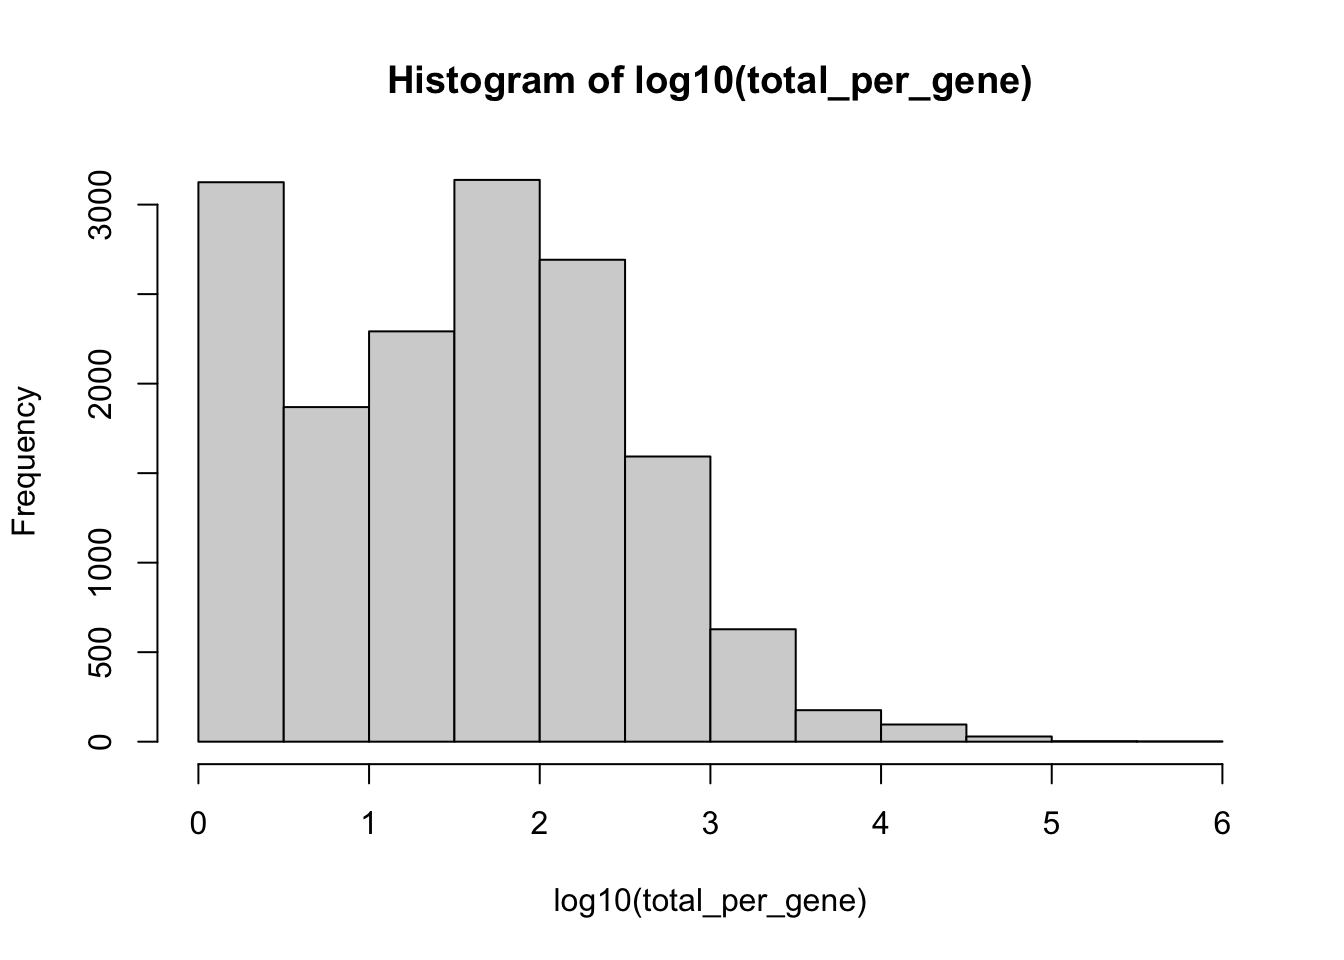
\includegraphics[keepaspectratio]{scRNAseqInR_ABACBS_2024_Doco_files/figure-latex/unnamed-chunk-49-1.pdf}}

Lets keep only those genes with at least 50 copies across the entire experiment.

\begin{Shaded}
\begin{Highlighting}[]
\NormalTok{seurat\_object}\OtherTok{\textless{}{-}}\NormalTok{ seurat\_object[total\_per\_gene }\SpecialCharTok{\textgreater{}=} \DecValTok{50}\NormalTok{, ] }
\end{Highlighting}
\end{Shaded}

How many genes after filtering?

\begin{Shaded}
\begin{Highlighting}[]
\NormalTok{seurat\_object}
\CommentTok{\#\textgreater{} An object of class Seurat }
\CommentTok{\#\textgreater{} 7200 features across 4877 samples within 1 assay }
\CommentTok{\#\textgreater{} Active assay: RNA (7200 features, 1236 variable features)}
\CommentTok{\#\textgreater{}  3 layers present: counts, data, scale.data}
\CommentTok{\#\textgreater{}  4 dimensional reductions calculated: pca, umap, harmony, umap\_harmony}
\end{Highlighting}
\end{Shaded}

We might like to see the effect of IFN-beta stimulation on each cell type individually. For the purposes of this workshop, just going to test one cell type; CD14+ Monocytes

An easy way is to subset the object.

\begin{Shaded}
\begin{Highlighting}[]
\CommentTok{\# Set idents to \textquotesingle{}cell\textquotesingle{} column.}
\FunctionTok{Idents}\NormalTok{(seurat\_object) }\OtherTok{\textless{}{-}}\NormalTok{ seurat\_object}\SpecialCharTok{$}\NormalTok{cell}
\FunctionTok{DimPlot}\NormalTok{(seurat\_object, }\AttributeTok{reduction =} \StringTok{"umap\_harmony"}\NormalTok{)}
\end{Highlighting}
\end{Shaded}

\pandocbounded{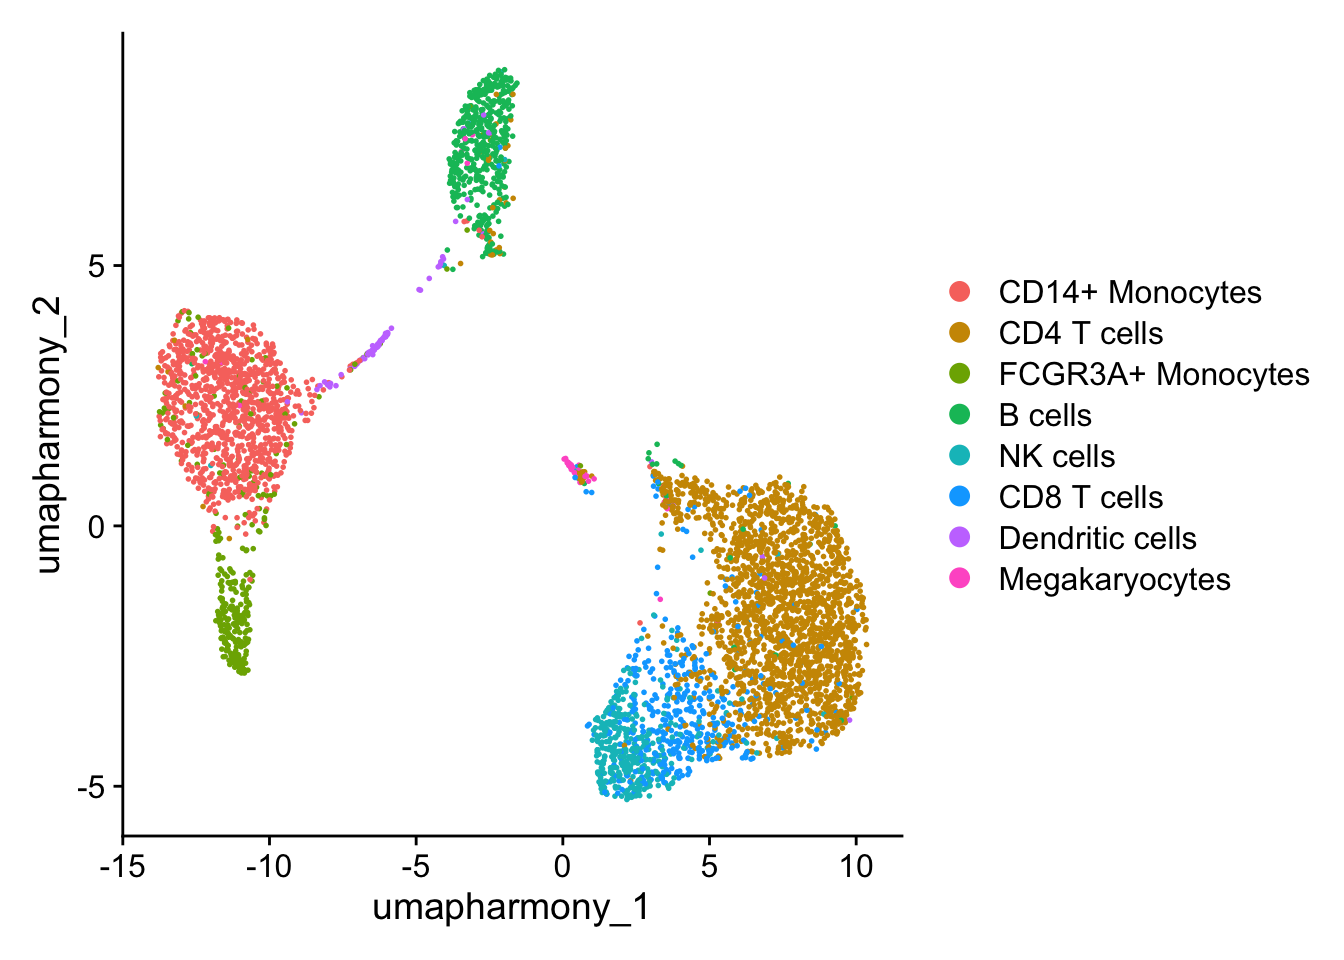
\includegraphics[keepaspectratio]{scRNAseqInR_ABACBS_2024_Doco_files/figure-latex/unnamed-chunk-52-1.pdf}}

\begin{Shaded}
\begin{Highlighting}[]
\NormalTok{seurat\_object\_celltype }\OtherTok{\textless{}{-}}\NormalTok{ seurat\_object[, seurat\_object}\SpecialCharTok{$}\NormalTok{cell }\SpecialCharTok{==} \StringTok{"CD14+ Monocytes"}\NormalTok{ ]}
\FunctionTok{DimPlot}\NormalTok{(seurat\_object\_celltype, }\AttributeTok{reduction =} \StringTok{"umap\_harmony"}\NormalTok{)}
\end{Highlighting}
\end{Shaded}

\pandocbounded{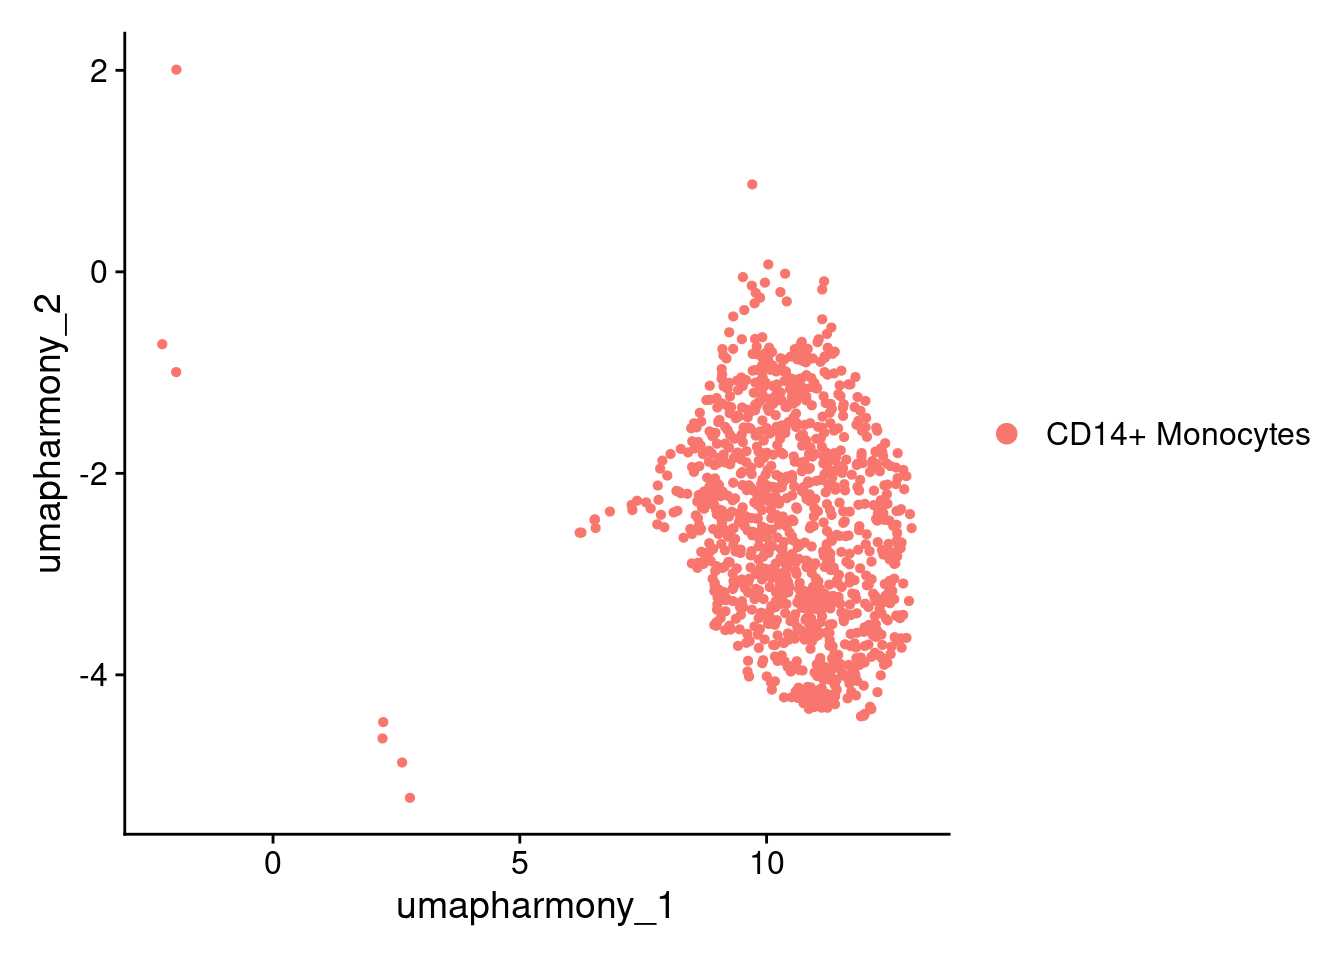
\includegraphics[keepaspectratio]{scRNAseqInR_ABACBS_2024_Doco_files/figure-latex/unnamed-chunk-52-2.pdf}}

\section{Default Wilcox test}\label{default-wilcox-test}

To run this test, we change the Idents to the factor(column) we want to test. In this case, that's `stim'.

\begin{Shaded}
\begin{Highlighting}[]
\CommentTok{\# Change Ident to Condition}
\FunctionTok{Idents}\NormalTok{(seurat\_object\_celltype) }\OtherTok{\textless{}{-}}\NormalTok{ seurat\_object\_celltype}\SpecialCharTok{$}\NormalTok{stim}

\CommentTok{\# default, wilcox test}
\NormalTok{de\_result\_wilcox }\OtherTok{\textless{}{-}} \FunctionTok{FindMarkers}\NormalTok{(seurat\_object\_celltype, }
            \AttributeTok{ident.1 =} \StringTok{\textquotesingle{}stim\textquotesingle{}}\NormalTok{,}
            \AttributeTok{ident.2 =} \StringTok{\textquotesingle{}ctrl\textquotesingle{}}\NormalTok{,}
            \AttributeTok{logfc.threshold =} \DecValTok{0}\NormalTok{, }\CommentTok{\# Give me ALL results}
            \AttributeTok{min.pct =} \DecValTok{0}
\NormalTok{            )}

\CommentTok{\# Add average expression for plotting}
\NormalTok{de\_result\_wilcox}\SpecialCharTok{$}\NormalTok{AveExpr}\OtherTok{\textless{}{-}} \FunctionTok{rowMeans}\NormalTok{(seurat\_object\_celltype[}\FunctionTok{rownames}\NormalTok{(de\_result\_wilcox),])}
\end{Highlighting}
\end{Shaded}

Look at the top differentially expressed genes.

\begin{Shaded}
\begin{Highlighting}[]
\FunctionTok{head}\NormalTok{(de\_result\_wilcox)}
\CommentTok{\#\textgreater{}                 p\_val avg\_log2FC pct.1 pct.2     p\_val\_adj}
\CommentTok{\#\textgreater{} RSAD2   8.471603e{-}196   6.797508 0.979 0.044 6.099554e{-}192}
\CommentTok{\#\textgreater{} TNFSF10 3.399691e{-}195   6.559853 0.982 0.056 2.447777e{-}191}
\CommentTok{\#\textgreater{} CXCL10  5.809758e{-}195   8.034949 0.975 0.038 4.183025e{-}191}
\CommentTok{\#\textgreater{} IFIT3   7.214495e{-}195   6.234703 0.982 0.051 5.194437e{-}191}
\CommentTok{\#\textgreater{} IFIT1   1.224398e{-}188   6.764699 0.953 0.026 8.815662e{-}185}
\CommentTok{\#\textgreater{} ISG15   1.228738e{-}186   6.377243 1.000 0.323 8.846914e{-}183}
\CommentTok{\#\textgreater{}            AveExpr}
\CommentTok{\#\textgreater{} RSAD2   0.04196286}
\CommentTok{\#\textgreater{} TNFSF10 0.51655832}
\CommentTok{\#\textgreater{} CXCL10  3.25184139}
\CommentTok{\#\textgreater{} IFIT3   0.02032398}
\CommentTok{\#\textgreater{} IFIT1   0.01254584}
\CommentTok{\#\textgreater{} ISG15   0.14165156}
\end{Highlighting}
\end{Shaded}

\begin{Shaded}
\begin{Highlighting}[]
\NormalTok{p1 }\OtherTok{\textless{}{-}} \FunctionTok{ggplot}\NormalTok{(de\_result\_wilcox, }\FunctionTok{aes}\NormalTok{(}\AttributeTok{x=}\NormalTok{AveExpr, }\AttributeTok{y=}\NormalTok{avg\_log2FC, }\AttributeTok{col=}\NormalTok{p\_val\_adj }\SpecialCharTok{\textless{}} \FloatTok{0.05}\NormalTok{)) }\SpecialCharTok{+}
  \FunctionTok{geom\_point}\NormalTok{() }\SpecialCharTok{+}
  \FunctionTok{scale\_colour\_manual}\NormalTok{(}\AttributeTok{values=}\FunctionTok{c}\NormalTok{(}\StringTok{\textquotesingle{}TRUE\textquotesingle{}}\OtherTok{=}\StringTok{"red"}\NormalTok{,}\StringTok{\textquotesingle{}FALSE\textquotesingle{}}\OtherTok{=}\StringTok{"black"}\NormalTok{)) }\SpecialCharTok{+} 
  \FunctionTok{theme\_bw}\NormalTok{() }\SpecialCharTok{+}
  \FunctionTok{ggtitle}\NormalTok{(}\StringTok{"Wilcox Test"}\NormalTok{)}


\NormalTok{p2 }\OtherTok{\textless{}{-}} \FunctionTok{ggplot}\NormalTok{(de\_result\_wilcox, }\FunctionTok{aes}\NormalTok{(}\AttributeTok{x=}\NormalTok{avg\_log2FC, }\AttributeTok{y=}\SpecialCharTok{{-}}\FunctionTok{log10}\NormalTok{(p\_val), }\AttributeTok{col=}\NormalTok{p\_val\_adj }\SpecialCharTok{\textless{}} \FloatTok{0.05}\NormalTok{)) }\SpecialCharTok{+}
  \FunctionTok{geom\_point}\NormalTok{() }\SpecialCharTok{+}
  \FunctionTok{scale\_colour\_manual}\NormalTok{(}\AttributeTok{values=}\FunctionTok{c}\NormalTok{(}\StringTok{\textquotesingle{}TRUE\textquotesingle{}}\OtherTok{=}\StringTok{"red"}\NormalTok{,}\StringTok{\textquotesingle{}FALSE\textquotesingle{}}\OtherTok{=}\StringTok{"black"}\NormalTok{)) }\SpecialCharTok{+} 
  \FunctionTok{theme\_bw}\NormalTok{() }\SpecialCharTok{+}
  \FunctionTok{ggtitle}\NormalTok{(}\StringTok{"Wilcox Test (Volcano)"}\NormalTok{)}

\NormalTok{p1 }\SpecialCharTok{+}\NormalTok{ p2}
\end{Highlighting}
\end{Shaded}

\pandocbounded{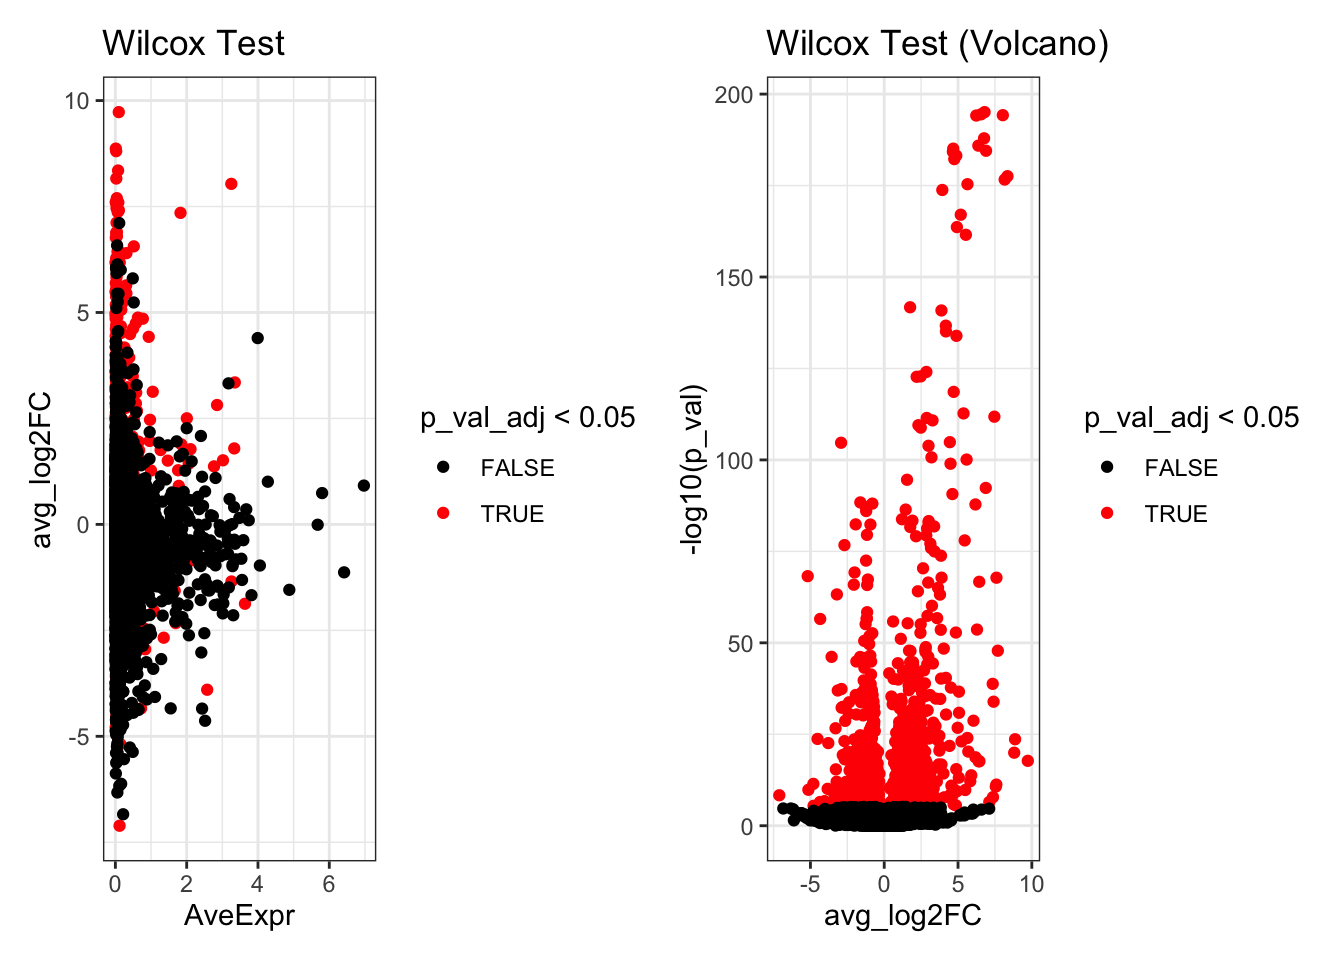
\includegraphics[keepaspectratio]{scRNAseqInR_ABACBS_2024_Doco_files/figure-latex/unnamed-chunk-55-1.pdf}}

\section{Seurat Negative binomial}\label{seurat-negative-binomial}

Negative binonial test is run almost the same way - just need to specify it under `test.use'

\begin{Shaded}
\begin{Highlighting}[]

\CommentTok{\# Change Ident to Condition}
\FunctionTok{Idents}\NormalTok{(seurat\_object\_celltype) }\OtherTok{\textless{}{-}}\NormalTok{ seurat\_object\_celltype}\SpecialCharTok{$}\NormalTok{stim}

\CommentTok{\# default, wilcox test}
\NormalTok{de\_result\_negbinom }\OtherTok{\textless{}{-}} \FunctionTok{FindMarkers}\NormalTok{(seurat\_object\_celltype, }
            \AttributeTok{test.use=}\StringTok{"negbinom"}\NormalTok{, }\CommentTok{\# Choose a different test.}
            \AttributeTok{ident.1 =} \StringTok{\textquotesingle{}stim\textquotesingle{}}\NormalTok{,}
            \AttributeTok{ident.2 =} \StringTok{\textquotesingle{}ctrl\textquotesingle{}}\NormalTok{,}
            \AttributeTok{logfc.threshold =} \DecValTok{0}\NormalTok{, }\CommentTok{\# Give me ALL results}
            \AttributeTok{min.pct =} \DecValTok{0}
\NormalTok{)}

\CommentTok{\# Add average expression for plotting}
\NormalTok{de\_result\_negbinom}\SpecialCharTok{$}\NormalTok{AveExpr}\OtherTok{\textless{}{-}} \FunctionTok{rowMeans}\NormalTok{(seurat\_object\_celltype[}\FunctionTok{rownames}\NormalTok{(de\_result\_negbinom),])}
\end{Highlighting}
\end{Shaded}

Look at the top differentially expressed genes.

\begin{Shaded}
\begin{Highlighting}[]
\FunctionTok{head}\NormalTok{(de\_result\_negbinom)}
\CommentTok{\#\textgreater{}          p\_val avg\_log2FC pct.1 pct.2 p\_val\_adj    AveExpr}
\CommentTok{\#\textgreater{} CXCL10       0   8.034949 0.975 0.038         0 0.04196286}
\CommentTok{\#\textgreater{} CCL8         0   8.160755 0.912 0.023         0 0.51655832}
\CommentTok{\#\textgreater{} LY6E         0   4.880093 0.979 0.134         0 3.25184139}
\CommentTok{\#\textgreater{} APOBEC3A     0   4.745713 0.996 0.262         0 0.02032398}
\CommentTok{\#\textgreater{} IFITM3       0   4.675898 0.998 0.271         0 0.01254584}
\CommentTok{\#\textgreater{} IFI6         0   3.935122 0.982 0.257         0 0.14165156}
\end{Highlighting}
\end{Shaded}

\begin{Shaded}
\begin{Highlighting}[]
\NormalTok{p1 }\OtherTok{\textless{}{-}} \FunctionTok{ggplot}\NormalTok{(de\_result\_negbinom, }\FunctionTok{aes}\NormalTok{(}\AttributeTok{x=}\NormalTok{AveExpr, }\AttributeTok{y=}\NormalTok{avg\_log2FC, }\AttributeTok{col=}\NormalTok{p\_val\_adj }\SpecialCharTok{\textless{}} \FloatTok{0.05}\NormalTok{)) }\SpecialCharTok{+}
  \FunctionTok{geom\_point}\NormalTok{() }\SpecialCharTok{+}
  \FunctionTok{scale\_colour\_manual}\NormalTok{(}\AttributeTok{values=}\FunctionTok{c}\NormalTok{(}\StringTok{\textquotesingle{}TRUE\textquotesingle{}}\OtherTok{=}\StringTok{"red"}\NormalTok{,}\StringTok{\textquotesingle{}FALSE\textquotesingle{}}\OtherTok{=}\StringTok{"black"}\NormalTok{)) }\SpecialCharTok{+} 
  \FunctionTok{theme\_bw}\NormalTok{() }\SpecialCharTok{+}
  \FunctionTok{ggtitle}\NormalTok{(}\StringTok{"Negative Bionomial Test"}\NormalTok{)}


\NormalTok{p2 }\OtherTok{\textless{}{-}} \FunctionTok{ggplot}\NormalTok{(de\_result\_negbinom, }\FunctionTok{aes}\NormalTok{(}\AttributeTok{x=}\NormalTok{avg\_log2FC, }\AttributeTok{y=}\SpecialCharTok{{-}}\FunctionTok{log10}\NormalTok{(p\_val), }\AttributeTok{col=}\NormalTok{p\_val\_adj }\SpecialCharTok{\textless{}} \FloatTok{0.05}\NormalTok{)) }\SpecialCharTok{+}
  \FunctionTok{geom\_point}\NormalTok{() }\SpecialCharTok{+}
  \FunctionTok{scale\_colour\_manual}\NormalTok{(}\AttributeTok{values=}\FunctionTok{c}\NormalTok{(}\StringTok{\textquotesingle{}TRUE\textquotesingle{}}\OtherTok{=}\StringTok{"red"}\NormalTok{,}\StringTok{\textquotesingle{}FALSE\textquotesingle{}}\OtherTok{=}\StringTok{"black"}\NormalTok{)) }\SpecialCharTok{+} 
  \FunctionTok{theme\_bw}\NormalTok{() }\SpecialCharTok{+}
  \FunctionTok{ggtitle}\NormalTok{(}\StringTok{"Negative Bionomial Test (Volcano)"}\NormalTok{)}

\NormalTok{p1 }\SpecialCharTok{+}\NormalTok{ p2}
\end{Highlighting}
\end{Shaded}

\pandocbounded{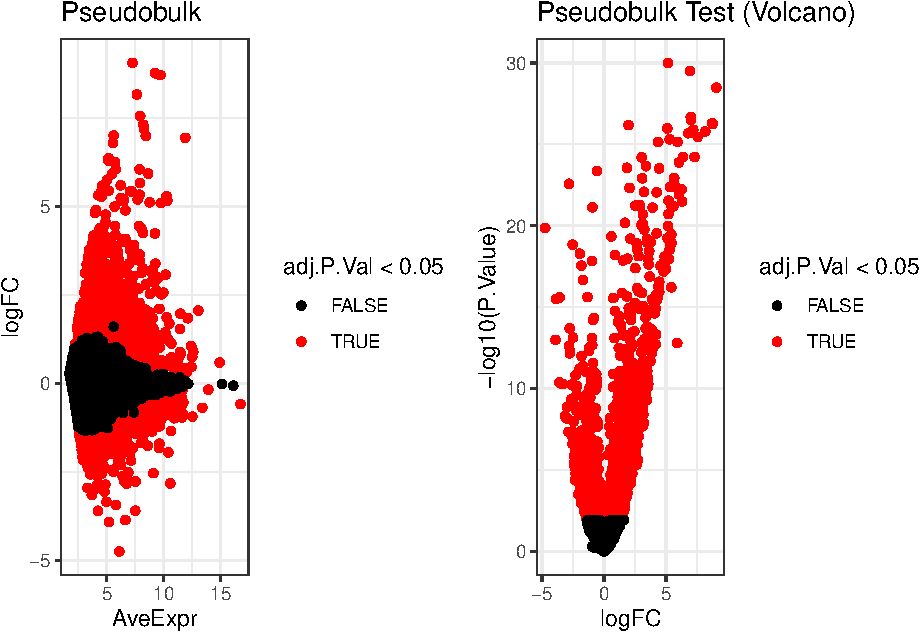
\includegraphics[keepaspectratio]{scRNAseqInR_ABACBS_2024_Doco_files/figure-latex/unnamed-chunk-58-1.pdf}}

\section{Pseudobulk}\label{pseudobulk}

Pseudobulk analysis is an option where you have biological replicates. It is essentially pooling the individual cell counts and treating your expreiment like a bulk RNAseq.

First, you need to build a pseudobulk matrix - the \texttt{AggregateExpression()} function can do this, once you set the `Idents' of your seurat object to your grouping factor (here, thats a combination of individual+treatment called `sample', instead of the `stim' treatment column).

\begin{Shaded}
\begin{Highlighting}[]
\CommentTok{\# Tools for bulk differential expression}
\FunctionTok{library}\NormalTok{(limma)}
\CommentTok{\#\textgreater{} }
\CommentTok{\#\textgreater{} Attaching package: \textquotesingle{}limma\textquotesingle{}}
\CommentTok{\#\textgreater{} The following object is masked from \textquotesingle{}package:BiocGenerics\textquotesingle{}:}
\CommentTok{\#\textgreater{} }
\CommentTok{\#\textgreater{}     plotMA}
\FunctionTok{library}\NormalTok{(edgeR)}
\CommentTok{\#\textgreater{} }
\CommentTok{\#\textgreater{} Attaching package: \textquotesingle{}edgeR\textquotesingle{}}
\CommentTok{\#\textgreater{} The following object is masked from \textquotesingle{}package:SingleCellExperiment\textquotesingle{}:}
\CommentTok{\#\textgreater{} }
\CommentTok{\#\textgreater{}     cpm}


\CommentTok{\# Change idents to ind for grouping.}
\NormalTok{seurat\_object\_celltype}\SpecialCharTok{$}\NormalTok{sample }\OtherTok{\textless{}{-}} \FunctionTok{factor}\NormalTok{(}\FunctionTok{paste}\NormalTok{(seurat\_object\_celltype}\SpecialCharTok{$}\NormalTok{stim, seurat\_object\_celltype}\SpecialCharTok{$}\NormalTok{ind, }\AttributeTok{sep=}\StringTok{"\_"}\NormalTok{))}
\FunctionTok{Idents}\NormalTok{(seurat\_object\_celltype) }\OtherTok{\textless{}{-}}\NormalTok{ seurat\_object\_celltype}\SpecialCharTok{$}\NormalTok{sample}

\CommentTok{\# THen pool together counts in those groups}
\CommentTok{\# AggregateExperssion returns a list of matricies {-} one for each assay requested (even just requesting one)}
\NormalTok{pseudobulk\_matrix\_list }\OtherTok{\textless{}{-}} \FunctionTok{AggregateExpression}\NormalTok{( seurat\_object\_celltype,  }\AttributeTok{slot =} \StringTok{\textquotesingle{}counts\textquotesingle{}}\NormalTok{, }\AttributeTok{assays=}\StringTok{\textquotesingle{}RNA\textquotesingle{}}\NormalTok{ )}
\CommentTok{\#\textgreater{} Names of identity class contain underscores (\textquotesingle{}\_\textquotesingle{}), replacing with dashes (\textquotesingle{}{-}\textquotesingle{})}
\CommentTok{\#\textgreater{} This message is displayed once every 8 hours.}
\NormalTok{pseudobulk\_matrix      }\OtherTok{\textless{}{-}}\NormalTok{ pseudobulk\_matrix\_list[[}\StringTok{\textquotesingle{}RNA\textquotesingle{}}\NormalTok{]]}
\NormalTok{pseudobulk\_matrix[}\DecValTok{1}\SpecialCharTok{:}\DecValTok{5}\NormalTok{,}\DecValTok{1}\SpecialCharTok{:}\DecValTok{4}\NormalTok{]}
\CommentTok{\#\textgreater{} 5 x 4 sparse Matrix of class "dgCMatrix"}
\CommentTok{\#\textgreater{}          ctrl{-}101 ctrl{-}1015 ctrl{-}1016 ctrl{-}1039}
\CommentTok{\#\textgreater{} NOC2L           2         7         .         .}
\CommentTok{\#\textgreater{} HES4            .         3         2         1}
\CommentTok{\#\textgreater{} ISG15          31       185       234        41}
\CommentTok{\#\textgreater{} TNFRSF18        .         3         4         2}
\CommentTok{\#\textgreater{} TNFRSF4         .         2         .         .}
\end{Highlighting}
\end{Shaded}

Now it looks like a bulk RNAseq experiment, so treat it like one.

We can use the popular \texttt{limma} package for differential expression. Here is one \href{https://ucdavis-bioinformatics-training.github.io/2018-June-RNA-Seq-Workshop/thursday/DE.html}{tutorial}, and the hefty reference manual is hosted by \href{https://bioconductor.org/packages/release/bioc/html/limma.html}{bioconductor}.

In brief, this code below constructs a linear model for this experiment that accounts for the variation in individuals and treatment. It then tests for differential expression between `stim' and `ctrl' groups.

\begin{Shaded}
\begin{Highlighting}[]
\NormalTok{dge }\OtherTok{\textless{}{-}} \FunctionTok{DGEList}\NormalTok{(pseudobulk\_matrix)}
\NormalTok{dge }\OtherTok{\textless{}{-}} \FunctionTok{calcNormFactors}\NormalTok{(dge)}

\CommentTok{\# Remove \_ or {-} and everything after it {-} yeilds stim group}
\NormalTok{stim }\OtherTok{\textless{}{-}} \FunctionTok{gsub}\NormalTok{(}\StringTok{"[{-}\_].*"}\NormalTok{,}\StringTok{""}\NormalTok{,}\FunctionTok{colnames}\NormalTok{(pseudobulk\_matrix)) }

\CommentTok{\# Removing everything before the \_ or {-} for the individual, then converting those numerical ind explictiy to text. Else limma will treat them as numbers!}
\NormalTok{ind  }\OtherTok{\textless{}{-}} \FunctionTok{as.character}\NormalTok{(}\FunctionTok{gsub}\NormalTok{(}\StringTok{".*[{-}\_]"}\NormalTok{,}\StringTok{""}\NormalTok{,}\FunctionTok{colnames}\NormalTok{(pseudobulk\_matrix))) }

\NormalTok{design }\OtherTok{\textless{}{-}} \FunctionTok{model.matrix}\NormalTok{( }\SpecialCharTok{\textasciitilde{}}\DecValTok{0} \SpecialCharTok{+}\NormalTok{ stim }\SpecialCharTok{+}\NormalTok{ ind)}
\NormalTok{vm  }\OtherTok{\textless{}{-}} \FunctionTok{voom}\NormalTok{(dge, }\AttributeTok{design =}\NormalTok{ design, }\AttributeTok{plot =} \ConstantTok{FALSE}\NormalTok{)}
\NormalTok{fit }\OtherTok{\textless{}{-}} \FunctionTok{lmFit}\NormalTok{(vm, }\AttributeTok{design =}\NormalTok{ design)}

\NormalTok{contrasts }\OtherTok{\textless{}{-}} \FunctionTok{makeContrasts}\NormalTok{(stimstim }\SpecialCharTok{{-}}\NormalTok{ stimctrl, }\AttributeTok{levels=}\FunctionTok{coef}\NormalTok{(fit))}
\NormalTok{fit }\OtherTok{\textless{}{-}} \FunctionTok{contrasts.fit}\NormalTok{(fit, contrasts)}
\NormalTok{fit }\OtherTok{\textless{}{-}} \FunctionTok{eBayes}\NormalTok{(fit)}

\NormalTok{de\_result\_pseudobulk }\OtherTok{\textless{}{-}} \FunctionTok{topTable}\NormalTok{(fit, }\AttributeTok{n =} \ConstantTok{Inf}\NormalTok{, }\AttributeTok{adjust.method =} \StringTok{"BH"}\NormalTok{)}
\NormalTok{de\_result\_pseudobulk }\OtherTok{\textless{}{-}} \FunctionTok{arrange}\NormalTok{(de\_result\_pseudobulk , adj.P.Val)}
\end{Highlighting}
\end{Shaded}

Look at the significantly differentially expressed genes:

\begin{Shaded}
\begin{Highlighting}[]
\FunctionTok{head}\NormalTok{(de\_result\_pseudobulk)}
\CommentTok{\#\textgreater{}           logFC   AveExpr        t      P.Value}
\CommentTok{\#\textgreater{} ISG20  5.161336 10.313033 35.72209 9.838370e{-}31}
\CommentTok{\#\textgreater{} ISG15  6.932960 11.897783 34.63778 3.049704e{-}30}
\CommentTok{\#\textgreater{} CXCL11 9.050139  7.263356 32.46019 3.282727e{-}29}
\CommentTok{\#\textgreater{} IFIT3  6.987552  8.423467 28.97126 2.052443e{-}27}
\CommentTok{\#\textgreater{} HERC5  6.999781  5.604886 28.65574 3.050588e{-}27}
\CommentTok{\#\textgreater{} CXCL10 8.708460  9.715253 28.25406 5.081902e{-}27}
\CommentTok{\#\textgreater{}           adj.P.Val        B}
\CommentTok{\#\textgreater{} ISG20  7.083626e{-}27 60.13277}
\CommentTok{\#\textgreater{} ISG15  1.097894e{-}26 59.02083}
\CommentTok{\#\textgreater{} CXCL11 7.878545e{-}26 55.45779}
\CommentTok{\#\textgreater{} IFIT3  3.694397e{-}24 52.01990}
\CommentTok{\#\textgreater{} HERC5  4.392847e{-}24 51.18902}
\CommentTok{\#\textgreater{} CXCL10 5.629458e{-}24 51.32019}
\end{Highlighting}
\end{Shaded}

\begin{Shaded}
\begin{Highlighting}[]
\NormalTok{p1 }\OtherTok{\textless{}{-}} \FunctionTok{ggplot}\NormalTok{(de\_result\_pseudobulk, }\FunctionTok{aes}\NormalTok{(}\AttributeTok{x=}\NormalTok{AveExpr, }\AttributeTok{y=}\NormalTok{logFC, }\AttributeTok{col=}\NormalTok{adj.P.Val }\SpecialCharTok{\textless{}} \FloatTok{0.05}\NormalTok{)) }\SpecialCharTok{+}
  \FunctionTok{geom\_point}\NormalTok{() }\SpecialCharTok{+}
  \FunctionTok{scale\_colour\_manual}\NormalTok{(}\AttributeTok{values=}\FunctionTok{c}\NormalTok{(}\StringTok{\textquotesingle{}TRUE\textquotesingle{}}\OtherTok{=}\StringTok{"red"}\NormalTok{,}\StringTok{\textquotesingle{}FALSE\textquotesingle{}}\OtherTok{=}\StringTok{"black"}\NormalTok{)) }\SpecialCharTok{+} 
  \FunctionTok{theme\_bw}\NormalTok{() }\SpecialCharTok{+}
  \FunctionTok{ggtitle}\NormalTok{(}\StringTok{"Pseudobulk"}\NormalTok{)}


\NormalTok{p2 }\OtherTok{\textless{}{-}} \FunctionTok{ggplot}\NormalTok{(de\_result\_pseudobulk, }\FunctionTok{aes}\NormalTok{(}\AttributeTok{x=}\NormalTok{logFC, }\AttributeTok{y=}\SpecialCharTok{{-}}\FunctionTok{log10}\NormalTok{(P.Value), }\AttributeTok{col=}\NormalTok{adj.P.Val }\SpecialCharTok{\textless{}} \FloatTok{0.05}\NormalTok{)) }\SpecialCharTok{+}
  \FunctionTok{geom\_point}\NormalTok{() }\SpecialCharTok{+}
  \FunctionTok{scale\_colour\_manual}\NormalTok{(}\AttributeTok{values=}\FunctionTok{c}\NormalTok{(}\StringTok{\textquotesingle{}TRUE\textquotesingle{}}\OtherTok{=}\StringTok{"red"}\NormalTok{,}\StringTok{\textquotesingle{}FALSE\textquotesingle{}}\OtherTok{=}\StringTok{"black"}\NormalTok{)) }\SpecialCharTok{+} 
  \FunctionTok{theme\_bw}\NormalTok{() }\SpecialCharTok{+}
  \FunctionTok{ggtitle}\NormalTok{(}\StringTok{"Pseudobulk Test (Volcano)"}\NormalTok{)}

\NormalTok{p1 }\SpecialCharTok{+}\NormalTok{ p2}
\end{Highlighting}
\end{Shaded}

\pandocbounded{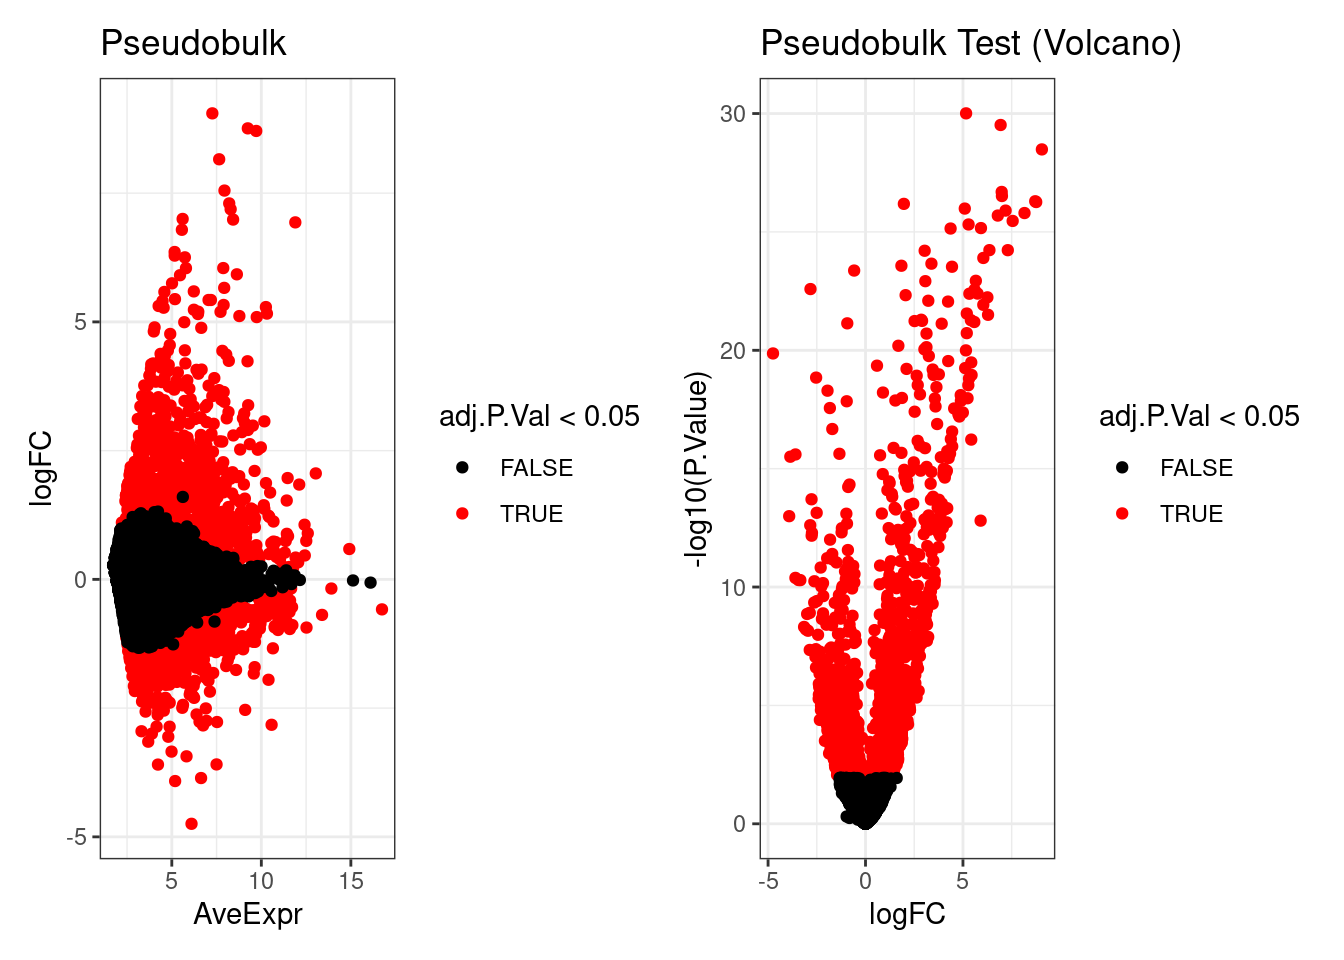
\includegraphics[keepaspectratio]{scRNAseqInR_ABACBS_2024_Doco_files/figure-latex/unnamed-chunk-62-1.pdf}}

\subsubsection*{Discussion}\label{discussion}
\addcontentsline{toc}{subsubsection}{Discussion}

These methods give different results. How would you decide which to use? How could you check an individual gene?

\subsubsection*{}\label{section-15}
\addcontentsline{toc}{subsubsection}{}

\chapter{Cell cycle Assignment}\label{CellCycle}

In some datasets, the phase of cell cycle that a cell is in (G1/G2M/S) can account for
alot of the observed transcriptomic variation. There may be clustering by phase, or
separation in the UMAP by phase.

Seurat provides a simple method for assigning cell cycle state to each cell. Other methods are available.

More information about assigning cell cycle states to cells is in the \href{https://satijalab.org/seurat/articles/cell_cycle_vignette.html}{cell cycle vignette}

\begin{Shaded}
\begin{Highlighting}[]
\CommentTok{\# A list of cell cycle markers, from Tirosh et al, 2015, is loaded with Seurat.  We can}
\CommentTok{\# segregate this list into markers of G2/M phase and markers of S phase}
\NormalTok{s.genes   }\OtherTok{\textless{}{-}}\NormalTok{ cc.genes}\SpecialCharTok{$}\NormalTok{s.genes}
\NormalTok{g2m.genes }\OtherTok{\textless{}{-}}\NormalTok{ cc.genes}\SpecialCharTok{$}\NormalTok{g2m.genes}

\CommentTok{\# Use those lists with the cell cycle scoring function in Seurat.}
\NormalTok{seurat\_object }\OtherTok{\textless{}{-}} \FunctionTok{CellCycleScoring}\NormalTok{(seurat\_object, }\AttributeTok{s.features =}\NormalTok{ s.genes, }\AttributeTok{g2m.features =}\NormalTok{ g2m.genes)}
\CommentTok{\#\textgreater{} Warning: The following features are not present in the}
\CommentTok{\#\textgreater{} object: TYMS, MCM2, MCM4, UNG, GINS2, CDCA7, DTL, UHRF1,}
\CommentTok{\#\textgreater{} MLF1IP, HELLS, RAD51AP1, GMNN, WDR76, CCNE2, ATAD2, RAD51,}
\CommentTok{\#\textgreater{} RRM2, CDC45, CDC6, EXO1, DSCC1, BLM, CASP8AP2, CLSPN,}
\CommentTok{\#\textgreater{} POLA1, CHAF1B, BRIP1, E2F8, not searching for symbol}
\CommentTok{\#\textgreater{} synonyms}
\CommentTok{\#\textgreater{} Warning: The following features are not present in the}
\CommentTok{\#\textgreater{} object: CDK1, NUSAP1, UBE2C, BIRC5, TPX2, TOP2A, NDC80,}
\CommentTok{\#\textgreater{} NUF2, MKI67, FAM64A, CCNB2, CKAP2L, AURKB, BUB1, KIF11,}
\CommentTok{\#\textgreater{} GTSE1, HJURP, CDCA3, CDC20, TTK, CDC25C, KIF2C, NCAPD2,}
\CommentTok{\#\textgreater{} DLGAP5, CDCA2, CDCA8, ECT2, KIF23, HMMR, AURKA, PSRC1,}
\CommentTok{\#\textgreater{} ANLN, CENPE, NEK2, GAS2L3, CENPA, not searching for symbol}
\CommentTok{\#\textgreater{} synonyms}
\end{Highlighting}
\end{Shaded}

Which adds S.Score, G2M.Score and Phase calls to the metadata.

\begin{Shaded}
\begin{Highlighting}[]
\FunctionTok{head}\NormalTok{(seurat\_object}\SpecialCharTok{@}\NormalTok{meta.data)}
\CommentTok{\#\textgreater{}                     orig.ident nCount\_RNA nFeature\_RNA  ind}
\CommentTok{\#\textgreater{} AGGGCGCTATTTCC{-}1 SeuratProject       2053          532 1256}
\CommentTok{\#\textgreater{} GGAGACGATTCGTT{-}1 SeuratProject        881          392 1256}
\CommentTok{\#\textgreater{} CACCGTTGTCGTAG{-}1 SeuratProject       3130         1005 1016}
\CommentTok{\#\textgreater{} TATCGTACACGCAT{-}1 SeuratProject       1042          549 1488}
\CommentTok{\#\textgreater{} TACGAGACCTATTC{-}1 SeuratProject       2425          777 1244}
\CommentTok{\#\textgreater{} GTACTACTCATACG{-}1 SeuratProject       3951         1064 1256}
\CommentTok{\#\textgreater{}                  stim              cell multiplets}
\CommentTok{\#\textgreater{} AGGGCGCTATTTCC{-}1 stim   CD14+ Monocytes    singlet}
\CommentTok{\#\textgreater{} GGAGACGATTCGTT{-}1 stim       CD4 T cells    singlet}
\CommentTok{\#\textgreater{} CACCGTTGTCGTAG{-}1 ctrl FCGR3A+ Monocytes    singlet}
\CommentTok{\#\textgreater{} TATCGTACACGCAT{-}1 stim           B cells    singlet}
\CommentTok{\#\textgreater{} TACGAGACCTATTC{-}1 stim       CD4 T cells    singlet}
\CommentTok{\#\textgreater{} GTACTACTCATACG{-}1 ctrl FCGR3A+ Monocytes    singlet}
\CommentTok{\#\textgreater{}                  percent.mt RNA\_snn\_res.0.5 seurat\_clusters}
\CommentTok{\#\textgreater{} AGGGCGCTATTTCC{-}1  1.6336634               1               0}
\CommentTok{\#\textgreater{} GGAGACGATTCGTT{-}1  4.8809524               5              15}
\CommentTok{\#\textgreater{} CACCGTTGTCGTAG{-}1  1.0655473               4              11}
\CommentTok{\#\textgreater{} TATCGTACACGCAT{-}1  3.0662710               3               5}
\CommentTok{\#\textgreater{} TACGAGACCTATTC{-}1  1.0837849               0               9}
\CommentTok{\#\textgreater{} GTACTACTCATACG{-}1  0.7137395               4              11}
\CommentTok{\#\textgreater{}                  pca\_clusters harmony\_clusters}
\CommentTok{\#\textgreater{} AGGGCGCTATTTCC{-}1            3                1}
\CommentTok{\#\textgreater{} GGAGACGATTCGTT{-}1            0                5}
\CommentTok{\#\textgreater{} CACCGTTGTCGTAG{-}1            9                4}
\CommentTok{\#\textgreater{} TATCGTACACGCAT{-}1            6                3}
\CommentTok{\#\textgreater{} TACGAGACCTATTC{-}1            0                0}
\CommentTok{\#\textgreater{} GTACTACTCATACG{-}1            9                4}
\CommentTok{\#\textgreater{}                  RNA\_snn\_res.0.1 RNA\_snn\_res.0.2}
\CommentTok{\#\textgreater{} AGGGCGCTATTTCC{-}1               1               1}
\CommentTok{\#\textgreater{} GGAGACGATTCGTT{-}1               0               0}
\CommentTok{\#\textgreater{} CACCGTTGTCGTAG{-}1               3               4}
\CommentTok{\#\textgreater{} TATCGTACACGCAT{-}1               2               3}
\CommentTok{\#\textgreater{} TACGAGACCTATTC{-}1               0               0}
\CommentTok{\#\textgreater{} GTACTACTCATACG{-}1               3               4}
\CommentTok{\#\textgreater{}                  RNA\_snn\_res.0.3 RNA\_snn\_res.0.4}
\CommentTok{\#\textgreater{} AGGGCGCTATTTCC{-}1               1               1}
\CommentTok{\#\textgreater{} GGAGACGATTCGTT{-}1               0               0}
\CommentTok{\#\textgreater{} CACCGTTGTCGTAG{-}1               4               4}
\CommentTok{\#\textgreater{} TATCGTACACGCAT{-}1               3               3}
\CommentTok{\#\textgreater{} TACGAGACCTATTC{-}1               0               0}
\CommentTok{\#\textgreater{} GTACTACTCATACG{-}1               4               4}
\CommentTok{\#\textgreater{}                  RNA\_snn\_res.0.6 RNA\_snn\_res.0.7}
\CommentTok{\#\textgreater{} AGGGCGCTATTTCC{-}1               1               1}
\CommentTok{\#\textgreater{} GGAGACGATTCGTT{-}1               7               6}
\CommentTok{\#\textgreater{} CACCGTTGTCGTAG{-}1               5               5}
\CommentTok{\#\textgreater{} TATCGTACACGCAT{-}1               3               3}
\CommentTok{\#\textgreater{} TACGAGACCTATTC{-}1               0               0}
\CommentTok{\#\textgreater{} GTACTACTCATACG{-}1               5               5}
\CommentTok{\#\textgreater{}                  RNA\_snn\_res.0.8 RNA\_snn\_res.0.9}
\CommentTok{\#\textgreater{} AGGGCGCTATTTCC{-}1               1               0}
\CommentTok{\#\textgreater{} GGAGACGATTCGTT{-}1               7               8}
\CommentTok{\#\textgreater{} CACCGTTGTCGTAG{-}1               6               7}
\CommentTok{\#\textgreater{} TATCGTACACGCAT{-}1               4               3}
\CommentTok{\#\textgreater{} TACGAGACCTATTC{-}1               0               1}
\CommentTok{\#\textgreater{} GTACTACTCATACG{-}1               6               7}
\CommentTok{\#\textgreater{}                  RNA\_snn\_res.1 RNA\_snn\_res.1.1}
\CommentTok{\#\textgreater{} AGGGCGCTATTTCC{-}1             1               0}
\CommentTok{\#\textgreater{} GGAGACGATTCGTT{-}1             9               9}
\CommentTok{\#\textgreater{} CACCGTTGTCGTAG{-}1             7               7}
\CommentTok{\#\textgreater{} TATCGTACACGCAT{-}1             3               3}
\CommentTok{\#\textgreater{} TACGAGACCTATTC{-}1             0               1}
\CommentTok{\#\textgreater{} GTACTACTCATACG{-}1             7               7}
\CommentTok{\#\textgreater{}                  RNA\_snn\_res.1.2 RNA\_snn\_res.1.3}
\CommentTok{\#\textgreater{} AGGGCGCTATTTCC{-}1               2               0}
\CommentTok{\#\textgreater{} GGAGACGATTCGTT{-}1               9              12}
\CommentTok{\#\textgreater{} CACCGTTGTCGTAG{-}1               7               9}
\CommentTok{\#\textgreater{} TATCGTACACGCAT{-}1               3               2}
\CommentTok{\#\textgreater{} TACGAGACCTATTC{-}1               0               8}
\CommentTok{\#\textgreater{} GTACTACTCATACG{-}1               7               9}
\CommentTok{\#\textgreater{}                  RNA\_snn\_res.1.4 RNA\_snn\_res.1.5}
\CommentTok{\#\textgreater{} AGGGCGCTATTTCC{-}1               0               0}
\CommentTok{\#\textgreater{} GGAGACGATTCGTT{-}1              14              14}
\CommentTok{\#\textgreater{} CACCGTTGTCGTAG{-}1              10              11}
\CommentTok{\#\textgreater{} TATCGTACACGCAT{-}1               2               2}
\CommentTok{\#\textgreater{} TACGAGACCTATTC{-}1               8               9}
\CommentTok{\#\textgreater{} GTACTACTCATACG{-}1              10              11}
\CommentTok{\#\textgreater{}                  RNA\_snn\_res.1.6 RNA\_snn\_res.1.7}
\CommentTok{\#\textgreater{} AGGGCGCTATTTCC{-}1               2               0}
\CommentTok{\#\textgreater{} GGAGACGATTCGTT{-}1              15              14}
\CommentTok{\#\textgreater{} CACCGTTGTCGTAG{-}1              12              11}
\CommentTok{\#\textgreater{} TATCGTACACGCAT{-}1               0               2}
\CommentTok{\#\textgreater{} TACGAGACCTATTC{-}1               9               9}
\CommentTok{\#\textgreater{} GTACTACTCATACG{-}1              12              11}
\CommentTok{\#\textgreater{}                  RNA\_snn\_res.1.8 RNA\_snn\_res.1.9}
\CommentTok{\#\textgreater{} AGGGCGCTATTTCC{-}1               0               4}
\CommentTok{\#\textgreater{} GGAGACGATTCGTT{-}1              14              16}
\CommentTok{\#\textgreater{} CACCGTTGTCGTAG{-}1              11              12}
\CommentTok{\#\textgreater{} TATCGTACACGCAT{-}1               2               0}
\CommentTok{\#\textgreater{} TACGAGACCTATTC{-}1              10               6}
\CommentTok{\#\textgreater{} GTACTACTCATACG{-}1              11              12}
\CommentTok{\#\textgreater{}                  RNA\_snn\_res.2 Naive\_CD4\_T1  cell\_label}
\CommentTok{\#\textgreater{} AGGGCGCTATTTCC{-}1             0   {-}0.3540023        \textless{}NA\textgreater{}}
\CommentTok{\#\textgreater{} GGAGACGATTCGTT{-}1            15    2.1376158 Naive\_CD4\_T}
\CommentTok{\#\textgreater{} CACCGTTGTCGTAG{-}1            11   {-}1.1487836        \textless{}NA\textgreater{}}
\CommentTok{\#\textgreater{} TATCGTACACGCAT{-}1             5    0.5557941        \textless{}NA\textgreater{}}
\CommentTok{\#\textgreater{} TACGAGACCTATTC{-}1             9    1.4250065 Naive\_CD4\_T}
\CommentTok{\#\textgreater{} GTACTACTCATACG{-}1            11   {-}0.2082793        \textless{}NA\textgreater{}}
\CommentTok{\#\textgreater{}                  SingleR.labels     S.Score   G2M.Score}
\CommentTok{\#\textgreater{} AGGGCGCTATTTCC{-}1       Monocyte {-}0.06808986 {-}0.08878508}
\CommentTok{\#\textgreater{} GGAGACGATTCGTT{-}1        T\_cells  0.09975063 {-}0.06812238}
\CommentTok{\#\textgreater{} CACCGTTGTCGTAG{-}1       Monocyte {-}0.12770457  0.16052598}
\CommentTok{\#\textgreater{} TATCGTACACGCAT{-}1    Neutrophils  0.08685571 {-}0.08316351}
\CommentTok{\#\textgreater{} TACGAGACCTATTC{-}1        T\_cells {-}0.02572695  0.02074759}
\CommentTok{\#\textgreater{} GTACTACTCATACG{-}1       Monocyte {-}0.07294007 {-}0.01517046}
\CommentTok{\#\textgreater{}                  Phase}
\CommentTok{\#\textgreater{} AGGGCGCTATTTCC{-}1    G1}
\CommentTok{\#\textgreater{} GGAGACGATTCGTT{-}1     S}
\CommentTok{\#\textgreater{} CACCGTTGTCGTAG{-}1   G2M}
\CommentTok{\#\textgreater{} TATCGTACACGCAT{-}1     S}
\CommentTok{\#\textgreater{} TACGAGACCTATTC{-}1   G2M}
\CommentTok{\#\textgreater{} GTACTACTCATACG{-}1    G1}
\end{Highlighting}
\end{Shaded}

We can then check the cell phase on the UMAP. In this dataset, phase isn't driving the clustering, and would not require any further handling.

\begin{Shaded}
\begin{Highlighting}[]
\FunctionTok{DimPlot}\NormalTok{(seurat\_object, }\AttributeTok{reduction =} \StringTok{\textquotesingle{}umap\_harmony\textquotesingle{}}\NormalTok{, }\AttributeTok{group.by =} \StringTok{"Phase"}\NormalTok{)}
\end{Highlighting}
\end{Shaded}

\pandocbounded{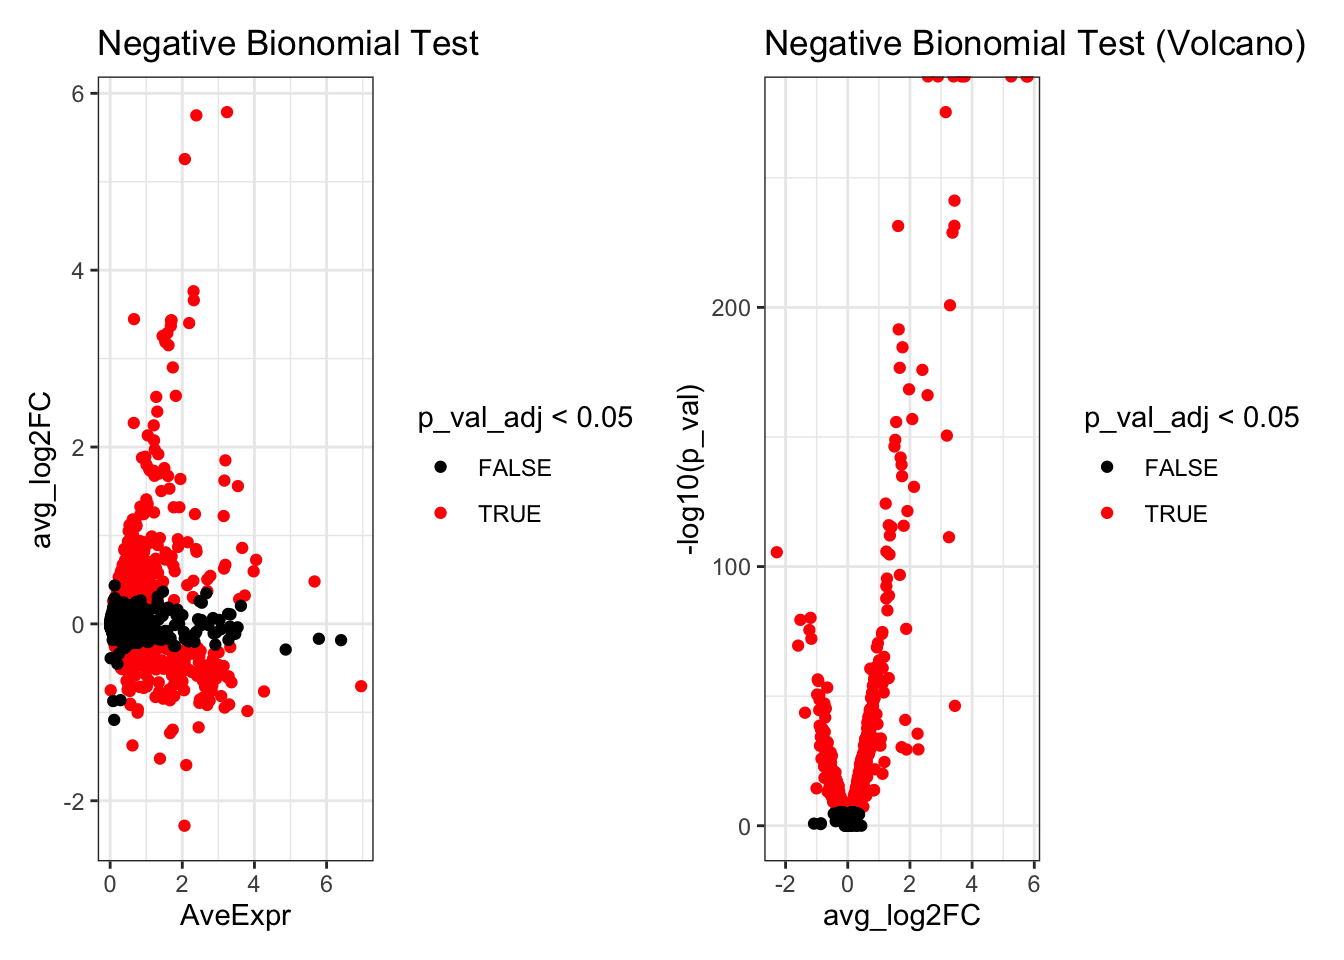
\includegraphics[keepaspectratio]{scRNAseqInR_ABACBS_2024_Doco_files/figure-latex/unnamed-chunk-65-1.pdf}}

Where a bias \emph{is} present, your course of action depends on the task at hand. It might involve `regressing out' the cell cycle variation when scaling data \texttt{ScaleData(kang,\ vars.to.regress="Phase")}, omitting cell-cycle dominated clusters, or just accounting for it in your differential expression calculations.

If you are working with non-human data, you will need to convert these gene lists, or find new cell cycle associated genes in your species.

\part{Other Resources}\label{part-other-resources}

\chapter{Resources}\label{resources}

Useful resources for next steps.

\subsection{Suggested Further Reading Material}\label{suggested-further-reading-material}

\begin{itemize}
\tightlist
\item
  \href{https://bioconductor.org/books/release/OSCA/}{Orchestrating Single Cell Analysis with Bioconductor} - this book teaches single cell analysis with the bioconductor ecosystem of packages rather than Seurat. Regardless of your preference for Bioconductor or Seurat, it provides an excellent grounding and further depth and rationale behind each step of a single cell analysis.
\item
  \href{https://satijalab.org/seurat/articles/get_started.html}{Seurat tutorials for gene expression, spatial \& multimodal analysis}
\item
  \href{https://satijalab.org/signac/articles/overview.html}{Getting started with Signac - the sibling package to Seurat for scATAC analysis}
\item
  \href{https://cole-trapnell-lab.github.io/monocle3/docs/trajectories/}{Monocle documentationn for trajectories}
\item
  \href{http://bioconductor.org/books/devel/SingleRBook/}{Cell Annotation with SingleR}
\item
  \href{https://immcantation.readthedocs.io/en/stable/}{VDJ analysis with Immcantation}
\end{itemize}

\subsection{Useful links arising from the discussion during the previous workshop}\label{useful-links-arising-from-the-discussion-during-the-previous-workshop}

\begin{itemize}
\tightlist
\item
  \href{https://kb.10xgenomics.com/hc/en-us/articles/218169723-What-fraction-of-reads-map-to-ribosomal-proteins-}{10x Genomics link to ribosomal protein expression}
\item
  \href{https://kb.10xgenomics.com/hc/en-us/articles/360001086611-Why-do-I-see-a-high-level-of-mitochondrial-gene-expression-}{10x Genomics link to mitochondrial gene expression}
\item
  \href{https://www.scrna-tools.org/}{scRNA Tools, catalogue of tools for scRNA Seq analysis}
\end{itemize}

\subsubsection{Data interpretation}\label{data-interpretation}

\begin{itemize}
\tightlist
\item
  \href{https://pair-code.github.io/understanding-umap/}{Interactive website explaining UMAP and comparision to t-SNE.}
\item
  \href{http://bioconductor.org/books/3.14/OSCA.basic/dimensionality-reduction.html\#visualization-interpretation}{OSCA, dimensionality reduction interpretation}
\item
  \href{https://logarithmic.net/2023/dimred.html}{A simple description of what PCA and UMAP do, with a 3D example.}
\end{itemize}

\subsubsection{Data tools and visualisation}\label{data-tools-and-visualisation}

\begin{itemize}
\tightlist
\item
  \href{https://satijalab.org/seurat/articles/sctransform_vignette.html}{scTransform Vignette}
\item
  \href{https://github.com/jdblischak/workflowr}{Link to the workflowr library}
\item
  \href{https://bioconductor.org/packages/release/bioc/html/iSEE.html}{iSEE Bioconductor library, interactive explorer}
\item
  \href{https://github.com/SGDDNB/ShinyCell}{ShinyCell makes interactive Shiny app from Seurat output}
\item
  \href{https://github.com/rezakj/iCellR}{iCellR interactive data explorer}
\item
  \href{https://www.helmholtz-munich.de/icb/research/groups/marr-lab/software/destiny/index.html}{Diffusion maps for single cell instead of umaps}
  *\href{https://logarithmic.net/langevitour/}{Projections of a high-dimensional dataset with an animated scatter-plot}
\end{itemize}

\subsubsection{Papers}\label{papers}

\begin{itemize}
\tightlist
\item
  \href{https://www.cell.com/cell-systems/fulltext/S2405-4712(20)30459-2}{Doublet cell detection method benchmarking paper.}
\item
  \href{https://www.nature.com/articles/s41598-019-41695-z}{From Louvain to Leiden: guaranteeing well-connected communities}
\end{itemize}

\subsubsection{Reference data and databases}\label{reference-data-and-databases}

\begin{itemize}
\tightlist
\item
  \href{https://gtexportal.org/home/}{Gene tissue expression database}
\item
  \href{https://www.immgen.org/Databrowser19/DatabrowserPage.html}{ImmGen Database and Explorer}
\item
  \href{https://singlecell.broadinstitute.org/single_cell}{Single Cell Study Portal from The Broad}
\item
  \href{http://bioconductor.org/packages/release/data/experiment/vignettes/celldex/inst/doc/userguide.html\#2_General-purpose_references}{Common ref data for cell indexing}
\item
  \href{https://azimuth.hubmapconsortium.org/references/\#Human\%20-\%20PBMC}{Azimuth is a Seurat-friendly reference-based annotation tool}
\item
  \href{https://www.bioconductor.org/packages/release/bioc/html/celaref.html}{Celaref, cell reference annotation tool}
\end{itemize}

\section{Help and fruther Resources}\label{help-and-fruther-resources}

\subsection*{Seurat Vignettes}\label{seurat-vignettes}
\addcontentsline{toc}{subsection}{Seurat Vignettes}

\url{https://satijalab.org/seurat/index.html}

There are a good many Seurat vigettes for different aspects of the Seurat package. E.g.

\begin{itemize}
\tightlist
\item
  \href{https://satijalab.org/seurat/articles/pbmc3k_tutorial.html}{Guided Clustering tutorial} : We've just worked through this
\item
  \href{https://satijalab.org/seurat/archive/v3.1/de_vignette.html}{Differential expression} : An Exploration of differential expression methods within Seurat
\item
  \href{https://satijalab.org/seurat/articles/integration_introduction.html}{Data integration} : Seurat's data integration is a popular method to combine different datasets into one joint analysis.
\end{itemize}

\subsection*{Seurat Cheatsheet}\label{seurat-cheatsheet}
\addcontentsline{toc}{subsection}{Seurat Cheatsheet}

\url{https://satijalab.org/seurat/articles/essential_commands.html}

A useful resource for asking; How can I do `X' with my seurat object?

\subsection*{OSCA}\label{osca}
\addcontentsline{toc}{subsection}{OSCA}

\url{https://bioconductor.org/books/release/OSCA/}

An comprehensive resource for analysis approaches for single cell data.
This uses the SingleCellExperiment bioconductor ecosystem, but alot of the same principle still apply.

This includes a good discussion of useing \href{http://bioconductor.org/books/3.15/OSCA.multisample/multi-sample-comparisons.html\#creating-pseudo-bulk-samples}{pseudobulk approaches}, worth checking out for differential expression analyses.

\subsection*{MBP training Reading list}\label{mbp-training-reading-list}
\addcontentsline{toc}{subsection}{MBP training Reading list}

\url{https://monashbioinformaticsplatform.github.io/Single-Cell-Workshop/}

A workshop page for a previous workshop (upon which this one is based) run by Monash Bioinformatics Platform - down the bottom there
is an extensive list of useful single cell links and resources.

\subsection*{Biocommons Single Cell Omics}\label{biocommons-single-cell-omics}
\addcontentsline{toc}{subsection}{Biocommons Single Cell Omics}

\url{https://www.biocommons.org.au/single-cell-omics}

Join the single cell omics community resources being setup by biocommons.

\begin{center}\rule{0.5\linewidth}{0.5pt}\end{center}

\section{Data}\label{data}

\subsection*{Demo 10X data}\label{demo-10x-data}
\addcontentsline{toc}{subsection}{Demo 10X data}

\url{https://www.10xgenomics.com/resources/datasets}

10X genomics have quite a few example datasets availble for download (including PBMC3k).
This is a useful resource if you want to see what the `raw' data looks like for a particular technology.

\subsection*{GEO}\label{geo}
\addcontentsline{toc}{subsection}{GEO}

\url{https://www.ncbi.nlm.nih.gov/geo/}

Many papers publish their raw single cell data in GEO. Formats vary, but often you can find the counts matrix.
\# (PART) Other resources \{-\}

\subsection*{Seurat data}\label{seurat-data}
\addcontentsline{toc}{subsection}{Seurat data}

\url{https://github.com/satijalab/seurat-data}

Package for obtaining a few datasets as seurat objects.

\begin{center}\rule{0.5\linewidth}{0.5pt}\end{center}

\section{Analysis Tools}\label{analysis-tools}

A handful of the many tools that might be worth checking out for next steps.

\subsection*{Cyclone}\label{cyclone}
\addcontentsline{toc}{subsection}{Cyclone}

\url{https://pubmed.ncbi.nlm.nih.gov/26142758/}

Part of the scran package, cyclone is a(nother) method for determining cell phase.
\href{https://rdrr.io/bioc/scran/man/cyclone.html}{Doco}

\subsection*{Harmony}\label{harmony}
\addcontentsline{toc}{subsection}{Harmony}

\url{https://portals.broadinstitute.org/harmony/articles/quickstart.html}

Method for integration of multiple single cell datasets.

\subsection*{SingleR}\label{singler-1}
\addcontentsline{toc}{subsection}{SingleR}

\url{http://bioconductor.org/books/release/SingleRBook/}

There is extensive documentation for the singleR package in the `singleR' book.

\subsection*{Scrublet}\label{scrublet}
\addcontentsline{toc}{subsection}{Scrublet}

\url{https://github.com/swolock/scrublet}

A python based tool for doublet detection. One of many tools in this space.

\subsection*{ScVelo}\label{scvelo}
\addcontentsline{toc}{subsection}{ScVelo}

\url{https://scvelo.readthedocs.io/}

A package for single cell RNA velocity analysis, useful for developmental/pseudotime trajectories. Python/scanpy based.

\subsection*{Monocle}\label{monocle}
\addcontentsline{toc}{subsection}{Monocle}

\url{https://cole-trapnell-lab.github.io/monocle3/}

A package for single cell developmental//pseudotime trajectory analysis.

\subsection*{TidySeurat}\label{tidyseurat}
\addcontentsline{toc}{subsection}{TidySeurat}

\url{https://stemangiola.github.io/tidyseurat/}

For fans of tidyverse-everything, there's tidyseurat. Example workflow \href{https://tidytranscriptomics-workshops.github.io/bioc2022_tidytranscriptomics/articles/tidytranscriptomics_case_study.html}{here}

\begin{center}\rule{0.5\linewidth}{0.5pt}\end{center}

\section{Preprocessing Tools}\label{preprocessing-tools}

Tooks that process raw sequencing data into counts matricies

\subsection*{Cell Ranger}\label{cell-ranger}
\addcontentsline{toc}{subsection}{Cell Ranger}

\url{https://support.10xgenomics.com/single-cell-gene-expression/software/pipelines/latest/what-is-cell-ranger}

CellRanger is the 10X tool that takes raw fastq sequence files and produces the counts matricies that are the starting point for today's analysis. It only works for 10X data.

\subsection*{STARSolo}\label{starsolo}
\addcontentsline{toc}{subsection}{STARSolo}

STAR is an aligner (which is actually used within cell ranger). STARSolo is a tool for producing counts matricies, and is configurable enough for use with multiple technologies.

\url{https://github.com/alexdobin/STAR/blob/master/docs/STARsolo.md}

\part{Seurat Object}\label{part-seurat-object}

\chapter{Structure}\label{structure}

\section{Load an existing Seurat object}\label{load-an-existing-seurat-object}

The data we're working with today is a small dataset of about 5000 PBMCs (peripheral blood mononuclear cells) from a healthy donor.

First, load Seurat package.

\begin{Shaded}
\begin{Highlighting}[]
\FunctionTok{library}\NormalTok{(Seurat)}
\end{Highlighting}
\end{Shaded}

And here's the one we prepared earlier. Seurat objects are usually saved as `.rds' files, which is an R format for storing binary data (not-text or human-readable). The functions \texttt{readRDS()} can load it.

\begin{Shaded}
\begin{Highlighting}[]
\NormalTok{seurat\_object }\OtherTok{\textless{}{-}} \FunctionTok{readRDS}\NormalTok{(}\StringTok{"data/kang2018.rds"}\NormalTok{)}
\end{Highlighting}
\end{Shaded}

\subsubsection*{Discussion: The Seurat Object in R}\label{discussion-the-seurat-object-in-r}
\addcontentsline{toc}{subsubsection}{Discussion: The Seurat Object in R}

Lets take a look at the seurat object we have just created in R, \texttt{seurat\_object}

To accomodate the complexity of data arising from a single cell RNA seq experiment, the seurat object keeps this as a container of multiple data tables that are linked.

\includegraphics[width=0.8\linewidth,height=\textheight,keepaspectratio]{images/seuratobject.png}

The functions in seurat can access parts of the data object for analysis and visualization, we will cover this later on.

There are a couple of concepts to discuss here.

\textbf{Class}

These are essentially data containers in R as a class, and can accessed as a variable in the R environment.

Classes are pre-defined and can contain multiple data tables and metadata. For Seurat, there are three types.

\begin{itemize}
\tightlist
\item
  Seurat - the main data class, contains all the data.
\item
  Assay - found within the Seurat object. Depending on the experiment a cell could have data on RNA, ATAC etc measured
\item
  DimReduc - for PCA and UMAP
\end{itemize}

\textbf{Slots}

Slots are parts within a class that contain specific data. These can be lists, data tables and vectors and can be accessed with conventional R methods.

\textbf{Data Access}

Many of the functions in Seurat operate on the data class and slots within them seamlessly. There maybe occasion to access these separately to \texttt{hack} them, however this is an advanced analysis method.

The ways to access the slots can be through methods for the class (functions) or with standard R accessor nomenclature.

\textbf{Examples of accessing a Seurat object}

The \texttt{assays} slot in \texttt{seurat\_object} can be accessed with \texttt{seurat\_object@assays}.

The \texttt{RNA} assay can be accessed from this with \texttt{seurat\_object@assays\$RNA}.

We often want to access assays, so Seurat nicely gives us a shortcut \texttt{seurat\_object\$RNA}. You may sometimes see an alternative notation \texttt{seurat\_object{[}{[}"RNA"{]}{]}}.

In general, slots that are always in an object are accessed with \texttt{@} and things that may be different in different data sets are accessed with \texttt{\$}.

\textbf{Have a go}

Use \texttt{str} to look at the structure of the Seurat object \texttt{seurat\_object}.

What is in the \texttt{meta.data} slot within your Seurat object currently? What type of data is contained here?

Where is our count data within the Seurat object?

\section{What's in there?}\label{whats-in-there}

Some of the most important information for working with Seurat objects is in the metadata.
This is cell level information - each row is one cell, identified by its barcode.
Extra information gets added to this table as analysis progresses.

\begin{Shaded}
\begin{Highlighting}[]
\FunctionTok{head}\NormalTok{(seurat\_object}\SpecialCharTok{@}\NormalTok{meta.data)}
\CommentTok{\#\textgreater{}                     orig.ident nCount\_RNA nFeature\_RNA  ind}
\CommentTok{\#\textgreater{} AGGGCGCTATTTCC{-}1 SeuratProject       2020          523 1256}
\CommentTok{\#\textgreater{} GGAGACGATTCGTT{-}1 SeuratProject        840          381 1256}
\CommentTok{\#\textgreater{} CACCGTTGTCGTAG{-}1 SeuratProject       3097          995 1016}
\CommentTok{\#\textgreater{} TATCGTACACGCAT{-}1 SeuratProject       1011          540 1488}
\CommentTok{\#\textgreater{} TGACGCCTTGCTTT{-}1 SeuratProject        570          367  101}
\CommentTok{\#\textgreater{} TACGAGACCTATTC{-}1 SeuratProject       2399          770 1244}
\CommentTok{\#\textgreater{}                  stim              cell multiplets}
\CommentTok{\#\textgreater{} AGGGCGCTATTTCC{-}1 stim   CD14+ Monocytes    singlet}
\CommentTok{\#\textgreater{} GGAGACGATTCGTT{-}1 stim       CD4 T cells    singlet}
\CommentTok{\#\textgreater{} CACCGTTGTCGTAG{-}1 ctrl FCGR3A+ Monocytes    singlet}
\CommentTok{\#\textgreater{} TATCGTACACGCAT{-}1 stim           B cells    singlet}
\CommentTok{\#\textgreater{} TGACGCCTTGCTTT{-}1 ctrl       CD4 T cells       ambs}
\CommentTok{\#\textgreater{} TACGAGACCTATTC{-}1 stim       CD4 T cells    singlet}
\end{Highlighting}
\end{Shaded}

That doesn't have any gene expression though, that's stored in an `Assay'.
The Assay structure has some nuances (see discussion below), but there are functions that get the assay data out for you.

By default this object will return the normalised data (from the only assay in this object, called RNA). Every `.' is a zero.

\begin{Shaded}
\begin{Highlighting}[]
\FunctionTok{GetAssayData}\NormalTok{(seurat\_object)[}\DecValTok{1}\SpecialCharTok{:}\DecValTok{15}\NormalTok{,}\DecValTok{1}\SpecialCharTok{:}\DecValTok{2}\NormalTok{]}
\CommentTok{\#\textgreater{} 15 x 2 sparse Matrix of class "dgCMatrix"}
\CommentTok{\#\textgreater{}               AGGGCGCTATTTCC{-}1 GGAGACGATTCGTT{-}1}
\CommentTok{\#\textgreater{} MIR1302{-}10                   .                .}
\CommentTok{\#\textgreater{} FAM138A                      .                .}
\CommentTok{\#\textgreater{} OR4F5                        .                .}
\CommentTok{\#\textgreater{} RP11{-}34P13.7                 .                .}
\CommentTok{\#\textgreater{} RP11{-}34P13.8                 .                .}
\CommentTok{\#\textgreater{} AL627309.1                   .                .}
\CommentTok{\#\textgreater{} RP11{-}34P13.14                .                .}
\CommentTok{\#\textgreater{} RP11{-}34P13.9                 .                .}
\CommentTok{\#\textgreater{} AP006222.2                   .                .}
\CommentTok{\#\textgreater{} RP4{-}669L17.10                .                .}
\CommentTok{\#\textgreater{} OR4F29                       .                .}
\CommentTok{\#\textgreater{} RP4{-}669L17.2                 .                .}
\CommentTok{\#\textgreater{} RP5{-}857K21.15                .                .}
\CommentTok{\#\textgreater{} RP5{-}857K21.1                 .                .}
\CommentTok{\#\textgreater{} RP5{-}857K21.2                 .                .}
\end{Highlighting}
\end{Shaded}

But the raw counts data is accessible too.

\begin{Shaded}
\begin{Highlighting}[]
\FunctionTok{GetAssayData}\NormalTok{(seurat\_object, }\AttributeTok{slot=}\StringTok{\textquotesingle{}counts\textquotesingle{}}\NormalTok{)[}\DecValTok{1}\SpecialCharTok{:}\DecValTok{15}\NormalTok{,}\DecValTok{1}\SpecialCharTok{:}\DecValTok{2}\NormalTok{]}
\CommentTok{\#\textgreater{} 15 x 2 sparse Matrix of class "dgCMatrix"}
\CommentTok{\#\textgreater{}               AGGGCGCTATTTCC{-}1 GGAGACGATTCGTT{-}1}
\CommentTok{\#\textgreater{} MIR1302{-}10                   .                .}
\CommentTok{\#\textgreater{} FAM138A                      .                .}
\CommentTok{\#\textgreater{} OR4F5                        .                .}
\CommentTok{\#\textgreater{} RP11{-}34P13.7                 .                .}
\CommentTok{\#\textgreater{} RP11{-}34P13.8                 .                .}
\CommentTok{\#\textgreater{} AL627309.1                   .                .}
\CommentTok{\#\textgreater{} RP11{-}34P13.14                .                .}
\CommentTok{\#\textgreater{} RP11{-}34P13.9                 .                .}
\CommentTok{\#\textgreater{} AP006222.2                   .                .}
\CommentTok{\#\textgreater{} RP4{-}669L17.10                .                .}
\CommentTok{\#\textgreater{} OR4F29                       .                .}
\CommentTok{\#\textgreater{} RP4{-}669L17.2                 .                .}
\CommentTok{\#\textgreater{} RP5{-}857K21.15                .                .}
\CommentTok{\#\textgreater{} RP5{-}857K21.1                 .                .}
\CommentTok{\#\textgreater{} RP5{-}857K21.2                 .                .}
\end{Highlighting}
\end{Shaded}

\chapter{Acknowledgements}\label{acknowledgements}

This material is mostly based on the \href{https://satijalab.org/seurat/articles/pbmc3k_tutorial.html}{Seurat introductory tutorial.}

It also draws from material for a \href{https://swbioinf.github.io/scRNAseqInR_Doco/index.html}{workshop provided by QCIF} developed by Sarah Williams and Ahmed Mehdi for the Australian Biocommons.

\chapter{Session info}\label{session-info}

\begin{Shaded}
\begin{Highlighting}[]

\FunctionTok{library}\NormalTok{(pander)}
\NormalTok{demo.Rmd\_session }\OtherTok{\textless{}{-}} \FunctionTok{sessionInfo}\NormalTok{()}
\FunctionTok{pander}\NormalTok{(demo.Rmd\_session)}
\end{Highlighting}
\end{Shaded}

\textbf{R version 4.4.0 (2024-04-24)}

\textbf{Platform:} x86\_64-pc-linux-gnu

\textbf{locale:}
\emph{LC\_CTYPE=en\_AU.UTF-8}, \emph{LC\_NUMERIC=C}, \emph{LC\_TIME=en\_AU.UTF-8}, \emph{LC\_COLLATE=en\_AU.UTF-8}, \emph{LC\_MONETARY=en\_AU.UTF-8}, \emph{LC\_MESSAGES=en\_AU.UTF-8}, \emph{LC\_PAPER=en\_AU.UTF-8}, \emph{LC\_NAME=C}, \emph{LC\_ADDRESS=C}, \emph{LC\_TELEPHONE=C}, \emph{LC\_MEASUREMENT=en\_AU.UTF-8} and \emph{LC\_IDENTIFICATION=C}

\textbf{attached base packages:}
\emph{stats4}, \emph{stats}, \emph{graphics}, \emph{grDevices}, \emph{utils}, \emph{datasets}, \emph{methods} and \emph{base}

\textbf{other attached packages:}
\emph{pander(v.0.6.6)}, \emph{edgeR(v.4.2.2)}, \emph{limma(v.3.60.6)}, \emph{celldex(v.1.14.0)}, \emph{SingleR(v.2.6.0)}, \emph{SingleCellExperiment(v.1.26.0)}, \emph{SummarizedExperiment(v.1.34.0)}, \emph{Biobase(v.2.64.0)}, \emph{GenomicRanges(v.1.56.2)}, \emph{GenomeInfoDb(v.1.40.1)}, \emph{IRanges(v.2.38.1)}, \emph{S4Vectors(v.0.42.1)}, \emph{BiocGenerics(v.0.50.0)}, \emph{MatrixGenerics(v.1.16.0)}, \emph{matrixStats(v.1.5.0)}, \emph{clustree(v.0.5.1)}, \emph{ggraph(v.2.2.1)}, \emph{harmony(v.1.2.3)}, \emph{Rcpp(v.1.1.0)}, \emph{future(v.1.67.0)}, \emph{patchwork(v.1.3.1)}, \emph{Seurat(v.5.3.0)}, \emph{SeuratObject(v.5.1.0)}, \emph{sp(v.2.2-0)}, \emph{ggplot2(v.3.5.2)} and \emph{dplyr(v.1.1.4)}

\textbf{loaded via a namespace (and not attached):}
\emph{spatstat.sparse(v.3.1-0)}, \emph{httr(v.1.4.7)}, \emph{RColorBrewer(v.1.1-3)}, \emph{tools(v.4.4.0)}, \emph{sctransform(v.0.4.2)}, \emph{backports(v.1.5.0)}, \emph{alabaster.base(v.1.4.2)}, \emph{utf8(v.1.2.6)}, \emph{R6(v.2.6.1)}, \emph{HDF5Array(v.1.32.1)}, \emph{lazyeval(v.0.2.2)}, \emph{uwot(v.0.2.3)}, \emph{rhdf5filters(v.1.16.0)}, \emph{withr(v.3.0.2)}, \emph{gridExtra(v.2.3)}, \emph{progressr(v.0.15.1)}, \emph{cli(v.3.6.5)}, \emph{spatstat.explore(v.3.5-2)}, \emph{fastDummies(v.1.7.5)}, \emph{alabaster.se(v.1.4.1)}, \emph{labeling(v.0.4.3)}, \emph{spatstat.data(v.3.1-6)}, \emph{ggridges(v.0.5.6)}, \emph{pbapply(v.1.7-4)}, \emph{parallelly(v.1.45.1)}, \emph{rstudioapi(v.0.17.1)}, \emph{RSQLite(v.2.4.2)}, \emph{generics(v.0.1.4)}, \emph{ica(v.1.0-3)}, \emph{spatstat.random(v.3.4-1)}, \emph{Matrix(v.1.7-0)}, \emph{ggbeeswarm(v.0.7.2)}, \emph{abind(v.1.4-8)}, \emph{lifecycle(v.1.0.4)}, \emph{yaml(v.2.3.10)}, \emph{rhdf5(v.2.48.0)}, \emph{SparseArray(v.1.4.8)}, \emph{BiocFileCache(v.2.12.0)}, \emph{Rtsne(v.0.17)}, \emph{grid(v.4.4.0)}, \emph{blob(v.1.2.4)}, \emph{promises(v.1.3.3)}, \emph{ExperimentHub(v.2.12.0)}, \emph{crayon(v.1.5.3)}, \emph{miniUI(v.0.1.2)}, \emph{lattice(v.0.22-6)}, \emph{beachmat(v.2.20.0)}, \emph{cowplot(v.1.2.0)}, \emph{KEGGREST(v.1.44.1)}, \emph{pillar(v.1.11.0)}, \emph{knitr(v.1.50)}, \emph{future.apply(v.1.20.0)}, \emph{codetools(v.0.2-20)}, \emph{glue(v.1.8.0)}, \emph{spatstat.univar(v.3.1-4)}, \emph{data.table(v.1.17.8)}, \emph{gypsum(v.1.0.1)}, \emph{vctrs(v.0.6.5)}, \emph{png(v.0.1-8)}, \emph{spam(v.2.11-1)}, \emph{gtable(v.0.3.6)}, \emph{cachem(v.1.1.0)}, \emph{xfun(v.0.52)}, \emph{S4Arrays(v.1.4.1)}, \emph{mime(v.0.13)}, \emph{tidygraph(v.1.3.1)}, \emph{survival(v.3.5-8)}, \emph{tinytex(v.0.57)}, \emph{statmod(v.1.5.0)}, \emph{fitdistrplus(v.1.2-4)}, \emph{ROCR(v.1.0-11)}, \emph{nlme(v.3.1-164)}, \emph{bit64(v.4.6.0-1)}, \emph{alabaster.ranges(v.1.4.2)}, \emph{filelock(v.1.0.3)}, \emph{RcppAnnoy(v.0.0.22)}, \emph{irlba(v.2.3.5.1)}, \emph{vipor(v.0.4.7)}, \emph{KernSmooth(v.2.23-22)}, \emph{colorspace(v.2.1-1)}, \emph{DBI(v.1.2.3)}, \emph{ggrastr(v.1.0.2)}, \emph{tidyselect(v.1.2.1)}, \emph{bit(v.4.6.0)}, \emph{compiler(v.4.4.0)}, \emph{curl(v.6.4.0)}, \emph{httr2(v.1.2.1)}, \emph{hdf5r(v.1.3.12)}, \emph{DelayedArray(v.0.30.1)}, \emph{plotly(v.4.11.0)}, \emph{bookdown(v.0.43)}, \emph{checkmate(v.2.3.2)}, \emph{scales(v.1.4.0)}, \emph{lmtest(v.0.9-40)}, \emph{rappdirs(v.0.3.3)}, \emph{stringr(v.1.5.1)}, \emph{digest(v.0.6.37)}, \emph{goftest(v.1.2-3)}, \emph{spatstat.utils(v.3.1-5)}, \emph{presto(v.1.0.0)}, \emph{alabaster.matrix(v.1.4.2)}, \emph{rmarkdown(v.2.29)}, \emph{XVector(v.0.44.0)}, \emph{RhpcBLASctl(v.0.23-42)}, \emph{htmltools(v.0.5.8.1)}, \emph{pkgconfig(v.2.0.3)}, \emph{sparseMatrixStats(v.1.16.0)}, \emph{dbplyr(v.2.5.0)}, \emph{fastmap(v.1.2.0)}, \emph{rlang(v.1.1.6)}, \emph{htmlwidgets(v.1.6.4)}, \emph{UCSC.utils(v.1.0.0)}, \emph{shiny(v.1.11.1)}, \emph{DelayedMatrixStats(v.1.26.0)}, \emph{farver(v.2.1.2)}, \emph{zoo(v.1.8-14)}, \emph{jsonlite(v.2.0.0)}, \emph{BiocParallel(v.1.38.0)}, \emph{BiocSingular(v.1.20.0)}, \emph{magrittr(v.2.0.3)}, \emph{GenomeInfoDbData(v.1.2.12)}, \emph{dotCall64(v.1.2)}, \emph{Rhdf5lib(v.1.26.0)}, \emph{viridis(v.0.6.5)}, \emph{reticulate(v.1.43.0)}, \emph{stringi(v.1.8.7)}, \emph{alabaster.schemas(v.1.4.0)}, \emph{zlibbioc(v.1.50.0)}, \emph{MASS(v.7.3-60.2)}, \emph{AnnotationHub(v.3.12.0)}, \emph{plyr(v.1.8.9)}, \emph{parallel(v.4.4.0)}, \emph{listenv(v.0.9.1)}, \emph{ggrepel(v.0.9.6)}, \emph{deldir(v.2.0-4)}, \emph{Biostrings(v.2.72.1)}, \emph{graphlayouts(v.1.2.2)}, \emph{splines(v.4.4.0)}, \emph{tensor(v.1.5.1)}, \emph{locfit(v.1.5-9.12)}, \emph{igraph(v.2.1.4)}, \emph{spatstat.geom(v.3.5-0)}, \emph{RcppHNSW(v.0.6.0)}, \emph{reshape2(v.1.4.4)}, \emph{ScaledMatrix(v.1.12.0)}, \emph{BiocVersion(v.3.19.1)}, \emph{evaluate(v.1.0.4)}, \emph{BiocManager(v.1.30.26)}, \emph{tweenr(v.2.0.3)}, \emph{httpuv(v.1.6.16)}, \emph{RANN(v.2.6.2)}, \emph{tidyr(v.1.3.1)}, \emph{purrr(v.1.1.0)}, \emph{polyclip(v.1.10-7)}, \emph{scattermore(v.1.2)}, \emph{ggforce(v.0.5.0)}, \emph{rsvd(v.1.0.5)}, \emph{xtable(v.1.8-4)}, \emph{RSpectra(v.0.16-2)}, \emph{later(v.1.4.2)}, \emph{viridisLite(v.0.4.2)}, \emph{tibble(v.3.3.0)}, \emph{memoise(v.2.0.1)}, \emph{beeswarm(v.0.4.0)}, \emph{AnnotationDbi(v.1.66.0)}, \emph{cluster(v.2.1.6)} and \emph{globals(v.0.18.0)}

  \bibliography{book.bib,packages.bib}

\end{document}
